% KZ \documentclass[letter,10pt, TexShade]{book} 
\documentclass[letter,12pt,TexShade,oneside]{book} 
\RequirePackage{fix-cm}
\usepackage{etex}
\usepackage{epsfig}
\usepackage{amsmath}
\usepackage{enumitem}
\usepackage{enumerate}
\usepackage{etex}
\usepackage[ruled,vlined,linesnumbered]{algorithm2e}
\usepackage{epsfig}
\usepackage{amsmath}
\usepackage[landscape]{geometry}
\usepackage{lscape}
\usepackage[pdfa,colorlinks=true,urlcolor=black]{hyperref}
\usepackage{tabularx}
\usepackage{gensymb}
%\usepackage{mathabx}
\usepackage{multirow}
\usepackage{moreverb}
\usepackage{multicol}
\usepackage{alltt}
\usepackage{setspace}
\usepackage{multirow}
\usepackage{lscape}
\usepackage[all]{xy}
\usepackage{color}
\usepackage{makeidx}
\usepackage{fancyvrb}
\usepackage{inputenc}
%\usepackage{dsfont}
\usepackage{moreverb}
\usepackage{array}
\usepackage{supertabular}
\usepackage{hhline}
\usepackage{rotating}
\hypersetup{colorlinks=true, linkcolor=Brown, citecolor=Brown, filecolor=Brown, urlcolor=Brown}
\usepackage{epsfig}
\usepackage{calc}
\usepackage{listings}
\usepackage[T1]{fontenc}
\usepackage{bm}
% \usepackage{amsthm}
\usepackage{theorem}
\usepackage{times,epsfig}
\usepackage{calc}
\usepackage{moresize}
%\usepackage[ruled]{algorithm2e}
\usepackage{url}
\usepackage{multirow}
\usepackage[bf,rm,medium,compact]{titlesec}
\usepackage{times}  
\usepackage{pifont}     % to include symbols from different fonts (e.g.  \rtm)
\usepackage{eurosym}    % for the euro symbol, package by Henrik Theiling
\usepackage{amstext}    % AMS for e.g. \text{}
\usepackage{graphicx}
\usepackage{booktabs}   % tables as required by journals
\usepackage{fancyhdr}                % fancy page headers/footers
\usepackage{vmargin}    % for \setmarginsrb                                      
\usepackage{xspace}
\usepackage{xcolor}

\usepackage{tikz}
\usepackage{pgfplots, pgf}
\usetikzlibrary{matrix,shapes,arrows,positioning}
%\usepackage{algorithm2e}
\usepackage{latex-pkg/postscript} % HV's elaboration of epsf
\usepackage[nolineno]{latex-pkg/lgrind}     % for typesetting MSL, Gentle, C, C++, ... code
\usepackage[grey]{latex-pkg/quotchap}
\usepackage{latex-pkg/TexShade}
%\usepackage[ruled]{algorithm2e}
%\usepackage[caption=false]{subfig}
\usepackage{subcaption}
\usepackage{cleveref}

\captionsetup[subfigure]{subrefformat=simple,labelformat=simple,skip=15pt,justification=raggedright}
\renewcommand\thesubfigure{(\alph{subfigure})}
\newcommand{\edited}[1]{\textbf{\color{blue} #1}}
\newcommand{\thcomment}[1]{\textbf{\color{magenta}COMMENT:}\textit{\color{magenta}  #1}}
\usepackage{url}
\usepackage{multirow}
\usepackage[bf,rm,medium,compact]{titlesec} % nice section titles
\usepackage{pifont}     % to include symbols from different fonts (e.g.  \rtm)
\usepackage{eurosym}    % for the euro symbol, package by Henrik Theiling
\usepackage{amstext}    % AMS for e.g. \text{}
\usepackage{booktabs}   % tables as required by journals
\usepackage{fancyhdr}                % fancy page headers/footers
\usepackage{vmargin}    % for \setmarginsrb                                      
\usepackage{latex-pkg/postscript} % HV's elaboration of epsf
\usepackage[nolineno]{latex-pkg/lgrind}     % for typesetting MSL, Gentle, C, C++, ... code
\usepackage[grey]{latex-pkg/quotchap}
\usepackage{latex-pkg/TexShade}
\usepackage{longtable}
\usepackage{ltcaption}
\usepackage{amsmath}
\DeclareMathOperator*{\argmax}{argmax}
\DeclareMathOperator*{\argmin}{argmin}
\DeclareMathOperator*{\expectval}{\mathbb{E}}
% The ltcaption package supports \CaptionLabelFont & \CaptionTextFont
% introduced by the NTG document classes
%\renewcommand\CaptionLabelFont{\normalsize}
%\renewcommand\CaptionTextFont{\normalsize}

%
%  Brown  Maroon  NavyBlue  MidnightBlue  
%

% INCLUDE HVs CUSTOMIZATIONS
%
% thesis.tex
%
% HV's thesis customisations
%
% for double sided printing, use book style.
% for single sided printing, use report style.
% This mainly has an inpact on the headings.

%% BEWARE of the order of the following packages !!
%% A different order may NOT work




% Modify algorithm package to HV's tastes
%\renewcommand{\algorithmicrequire}{\textbf{\textsf{Require:}}}
%\renewcommand{\algorithmicensure}{\textbf{\textsf{Ensure:}}}
%\renewcommand{\algorithmicend}{\textbf{\textsf{end}}}
%\renewcommand{\algorithmicif}{\textbf{\textsf{if}}}
%\renewcommand{\algorithmicthen}{\textbf{\textsf{then}}}
%\renewcommand{\algorithmicelse}{\textbf{\textsf{else}}}
%\renewcommand{\algorithmicelsif}{\algorithmicelse\ \algorithmicif}
%\renewcommand{\algorithmicendif}{\algorithmicend\ \algorithmicif}
%\renewcommand{\algorithmicfor}{\textbf{\textsf{for}}}
%\renewcommand{\algorithmicforall}{\textbf{\textsf{for all}}}
%\renewcommand{\algorithmicdo}{\textbf{\textsf{do}}}
%\renewcommand{\algorithmicendfor}{\algorithmicend\ \algorithmicfor}
%\renewcommand{\algorithmicwhile}{\textbf{\textsf{while}}}
%\renewcommand{\algorithmicendwhile}{\algorithmicend\ \algorithmicwhile}
%\renewcommand{\algorithmicloop}{\textbf{\textsf{loop}}}
%\renewcommand{\algorithmicendloop}{\algorithmicend\ \algorithmicloop}
%\renewcommand{\algorithmicrepeat}{\textbf{\textsf{repeat}}}
%\renewcommand{\algorithmicuntil}{\textbf{\textsf{until}}}
%
%\renewcommand{\algorithmiccomment}[1]{\hfill \{#1\}}

% to test if in TTH (HTML generation)
\newif\iftth
% to have MathBlackboardBold in TeX, Calligraphic in TTH
\newcommand{\bb}[1]{\iftth\cal{#1}\else\mathbb{#1}\fi}

% Currently, to fit as much on a page as possible
%
%\setpapersize{A4} % necessary when using a4paper ?
\setpapersize{USletter}


%
% KZ \setmarginsrb{3cm}{1.7cm}{2.2cm}{2.7cm}
% KZ 	     {12pt}{25pt}{12pt}{40pt}
%

%\setmarginsrb{3cm}{1.7cm}{2.2cm}{2.7cm}
%	     {12pt}{25pt}{12pt}{40pt}


%
%% \setmarginsrb{leftmargin}{topmargin}{rightmargin}{bottommargin}%
%%              {headheight}{headsep}{footheight}{footskip}
%
% KZ
%
%\setmarginsrb{38mm}{25mm}{25mm}{25mm}%
%	     {12pt}{25pt}{12pt}{40pt}


%%%%%%%%%%%%%%%%%%%%%%%%%%%%%%%%%%%%%%%%%%%%%%%
%
% Printed Feb 25
%
%\setmarginsrb{36mm}{30mm}{24mm}{35mm}%
%	      {12pt}{25pt}{12pt}{40pt}
%
%%%%%%%%%%%%%%%%%%%%%%%%%%%%%%%%%%%%%%%%%%%%%%%


%% \setmarginsrb{leftmargin}{topmargin}{rightmargin}{bottommargin}%
%%              {headheight}{headsep}{footheight}{footskip}

%
% KZ Working
%
%\setmarginsrb{36mm}{34mm}{22mm}{34mm}%
%	     {12pt}{30pt}{12pt}{40pt}




%
% KZ Working 222
%
% \setmarginsrb{36mm}{28mm}{22mm}{35mm}%
%	     {30pt}{20pt}{12pt}{40pt}
%

%
%\setmarginsrb{36mm}{28mm}{22mm}{35mm}%
%	     {30pt}{20pt}{12pt}{40pt}
%

%\setmarginsrb{1}{2}{3}{4}{5}{6}{7}{8}
%1 est la marge gauche
%2 est la marge en haut
%3 est la marge droite
%4 est la marge en bas
%5 fixe la hauteur de l'entête
%6 fixe la distance entre l'entête et le texte
%7 fixe la hauteur du pied de page
%8 fixe la distance entre le texte et le pied de page

% ADAPT BY JULIEN FOR LETTER PAPER INSTEAD OF A4
\setmarginsrb{22mm}{20mm}{22mm}{28mm}%
	     {30pt}{20pt}{12pt}{40pt}



% HV's manual adjustments were
%\textwidth 16.5cm
%\textheight 24.2cm
%\topmargin -1.8cm
%\oddsidemargin 0.cm

%% standard scaling factor for included PostScript
\newcommand{\epsscale}{0.7}

% HV prefers not to indent paragraphs and skip only a little
% KZ \parindent 0.cm
% KZ \parskip 0.1cm


%\parindent 0.0cm
\parskip   0.25cm





% To refer to the section etc. AND to the page,
% use consistently only when referring into other chapter.
%
\newcommand{\fullref}[1]{\ref{#1} on page~\pageref{#1}}

%
% We don't want double space after end of sentence punctuation
%
\frenchspacing

% Normal itemize takes too much space
%
%\renewenvironment{itemize}%
%  {\begin{list}{$\bullet$}%
%               {\setlength{\parsep}{0pt}
%                \setlength{\itemsep}{0pt}}}%
%  {\end{list}}

% TM sign
%\def\rtm{$^{\text{\Pisymbol{psy}{226}}}$} % The ``registered trademark sign''

%% For formatting semantic definitions
%  HV: keep this or change ?
%
\newcommand{\enum}{\ \textbf{enum}\ }
\newcommand{\myif}{\ \textbf{if}\ }
\newcommand{\myelse}{\ \textbf{else}\ }

\newcommand{\defbegin}[1]{\begin{center}{\bf {\sf #1}}\end{center}
 \hrule {\bf {\sf Syntax:}} \vspace{-0.2cm}}
\newenvironment{semantics}{\vspace{-0.7cm}
 {\bf {\sf Semantics:} \vspace{-0.2cm}}
 \begin{quote}}{\end{quote}}
\newcommand{\defobject}{\vspace{-0.7cm}{\bf {\sf Object:}
\vspace{-0.2cm}}}
\renewenvironment{object}{\vspace{-0.7cm}{\bf {\sf Object:}
\vspace{-0.2cm}}  
 \begin{quote}}{\end{quote}}
\newcommand{\defend}{\hrule~\\}

%% Miscellaneous preamble information

\newcommand{\vb}[1]{\verb+#1+}
\newcommand{\st}[1]{{\em #1\/}}
\newcommand{\ic}{{\em i.c.,\ }}
\newcommand{\ie}{{\em i.e.,\ }}
\newcommand{\eg}{{\em e.g.,\ }}
\newcommand{\vs}{{\em vs.\ }}
\newcommand{\cfr}{{\em cfr.\ }}
\newcommand{\etc}{{\em ,\ etc.\ }}
\newcommand{\beq}{\begin{equation}}
\newcommand{\eeq}{\end{equation}}
\newcommand{\beqa}{\begin{eqnarray}}
\newcommand{\eeqa}{\end{eqnarray}}

\renewcommand{\contentsname}{{\huge\rm\bfseries{Contents}}}
\renewcommand{\listfigurename}{{\huge\rm\bfseries{List of Figures}}}
\renewcommand{\listtablename}{{\huge\rm\bfseries{List of Tables}}}
%\renewcommand{\listalgorithmname}{{\huge\rm\bfseries{List of Algorithms}}}
\renewcommand{\bibname}{{\rm\bfseries{Bibliography}}}






% End of File defaultcustom.tex









% INCLUDE LATEX PACKAGES

\makeatletter
\newcommand\arraybslash{\let\\\@arraycr}
%\@addtoreset{chapter}{part}
\makeatother



\lstset{basicstyle=\normalsize\ttfamily,breaklines=true}
\lstset{framextopmargin=5pt,frame=bottomline}


%[latin1]
% INCLUDE LATEX PREAMBLE
% SETTINGS FOR listings PACKAGE
\lstset{
    numberstyle=\tiny,
    numbers=left,
    stepnumber=1,
    numbersep=5pt,
    tabsize=2,
    showstringspaces=false,
    aboveskip=\smallskipamount,
    belowskip=\smallskipamount,
    lineskip=-2pt
}

% PAGE COLOR and SETTINGSx
\pagecolor{white}

% \setlength{\headheight}{2cm}
% \setlength{\marginparwidth}{1.9cm}
% MAKE INDEX
\makeindex

% CUSTOM COMMANDS
\newcommand{\linka}[1]{{\tt\htmladdnormallink{#1}{#1}}}
\newcommand{\linkb}[2]{{\tt\htmladdnormallink{#1}{#2}}}
\newcommand{\parcomment}[1]{\marginpar{\scriptsize{\textcolor{blue}{#1}}}}
\newcommand{\defn}[2]{{\begin{minipage}{\textwidth}\vspace{2pt}\emph{\textbf{#1}}:\vspace{1pt}\begin{center}\fbox{\begin{minipage}{5.5in}#2\end{minipage}}\end{center}\vspace{2pt}\end{minipage}}}

% lgrind FONTS
\def\BGfont{\small\tt}
\def\CMfont{\small\tt}
\def\NOfont{\small\tt}
\def\KWfont{\small\tt}
\def\STfont{\small\tt}
\def\TTfont{\small\tt}
\def\VRfont{\small\tt}

% KZ definitions
%%%%%%%%%%%%%%%%%%%%%%%%%%%%%%%%%%%%%%%%%%%%%%%%%%
%
%  KZ  BEGIN  PARAMS  1
%
%%%%%%%%%%%%%%%%%%%%%%%%%%%%%%%%%%%%%%%%%%%%%%%%%%


% \theoremstyle{break}


%%%%%%%%%%%%%%%%%%%%%
%
%  new-theorem-0
%
%%%%%%%%%%%%%%%%%%%%%

\theoremstyle{plain}
\theorembodyfont{\normalfont}
\newtheorem{mytheorem-0}{\textsc{Theorem}}\numberwithin{mytheorem-0}{section}


\newenvironment{new-theorem-0}
{
\begin{mytheorem-0}
\begin{quote}
}
{
\end{quote}
\end{mytheorem-0}
}

%%%%%%%%%%%%%%%%%%%%%


%%%%%%%%%%%%%%%%%%%%%
%
%  new-corollary-0
%
%%%%%%%%%%%%%%%%%%%%%

\theoremstyle{plain}
\theorembodyfont{\normalfont}
\newtheorem{mycorollary-0}{\textsc{Corollary}}
\numberwithin{mycorollary-0}{section}


\newenvironment{new-corollary-0}
{
\begin{mycorollary-0}
\begin{quote}
}
{
\end{quote}
\end{mycorollary-0}
}

%%%%%%%%%%%%%%%%%%%%%



%%%%%%%%%%%%%%%%%%%%%
%
%  new-proposition-0
%
%%%%%%%%%%%%%%%%%%%%%

\theoremstyle{plain}
\theorembodyfont{\normalfont}
\newtheorem{myproposition-0}{\textsc{Proposition}}\numberwithin{myproposition-0}
{section}


\newenvironment{new-proposition-0}
{
\begin{myproposition-0}
\begin{quote}
}
{
\end{quote}
\end{myproposition-0}
}

%%%%%%%%%%%%%%%%%%%%%






%%%%%%%%%%%%%%%%%%%%%
%
%  new-lemma-0
%
%%%%%%%%%%%%%%%%%%%%%

\theoremstyle{plain}
\theorembodyfont{\normalfont}
\newtheorem{mylemma-0}{\textsc{Lemma}}
\numberwithin{mylemma-0}{section}


\newenvironment{new-lemma-0}
{
\begin{mylemma-0}
\begin{quote}
}
{
\end{quote}
\end{mylemma-0}
}

%%%%%%%%%%%%%%%%%%%%%




%%%%%%%%%%%%%%%%%%%%%
%
%  new-definition-0
%
%%%%%%%%%%%%%%%%%%%%%

\theoremstyle{plain}
\theorembodyfont{\normalfont}
\newtheorem{mydefinition-0}{\textsc{Definition}}
\numberwithin{mydefinition-0}{section}



\newenvironment{new-definition-0}
{
\begin{mydefinition-0}
\begin{quote}
}
{
\end{quote}
\end{mydefinition-0}
}

%%%%%%%%%%%%%%%%%%%%%




\newenvironment{new-proof-0}{
\noindent{\textbf{\textit{Proof.}}}
\begin{quote}
}
{
\end{quote}
}





%%%%%%%%%%%%%%%%%%%%%%%%%%%%%%%%%%%%%%%%%%%%%%%%%%
%
%  KZ  END  PARAMS  1
%
%%%%%%%%%%%%%%%%%%%%%%%%%%%%%%%%%%%%%%%%%%%%%%%%%%















%%%%%%%%%%%%%%%%%%%%%%%%%%%%%%%%%%%%%%%%%%%%%%%%%%
%
%  KZ  BEGIN  PARAMS  2
%
%%%%%%%%%%%%%%%%%%%%%%%%%%%%%%%%%%%%%%%%%%%%%%%%%%



\newcounter{theoremCounter}
\setcounter{theoremCounter}{0}
\newenvironment{new-theorem-1}
{% This is the begin code
\stepcounter{theoremCounter}
{\noindent}{\textbf{\textsc{Theorem}}} \arabic{theoremCounter}.
}
{}





%
% Corollary
%
\newcounter{corollaryCounter}
\setcounter{corollaryCounter}{0}
\newenvironment{new-corollary-1}
{% This is the begin code
\stepcounter{corollaryCounter}
{\noindent}{\textbf{\textsc{Corollary}}} \arabic{corollaryCounter}.
}
{}



%
% Lemma
%
\newcounter{lemmaCounter}
\setcounter{lemmaCounter}{0}
\newenvironment{new-lemma-1}
{% This is the begin code
\stepcounter{lemmaCounter}
{\noindent}{\textbf{\textsc{Lemma}}} \arabic{lemmaCounter}.
}
{}



%
% Proposition
%
\newcounter{propositionCounter}
\setcounter{propositionCounter}{0}
\newenvironment{new-proposition-1}
{% This is the begin code
\stepcounter{propositionCounter}
{\noindent}{\textbf{\textsc{Proposition}}} \arabic{propositionCounter}.
}
{}




%
% Definition
%

\newcounter{definitionCounter}
\setcounter{definitionCounter}{0}
\newenvironment{new-definition-1}
{
\stepcounter{definitionCounter}
{\noindent}{\textbf{\textsc{Definition}}} \arabic{definitionCounter}.
}
{}

%\hfill\qed\vspace{0.1cm}}






\newenvironment{new-proof-1}{
\noindent{\textbf{\textit{Proof.}}}}
{}



% \newtheorem{theorem}{Theorem}[section]
% \newtheorem{new-lemma-0}[theorem]{Proposition}
% \newtheorem{new-definition-0}[theorem]{Definition}









\newenvironment{new-item}%
{\begin{list}{$\bullet$}{%
\topsep0pt \partopsep0pt \parsep0pt \itemsep0.1ex plus 0.1ex minus 0.1ex
\setlength{\leftmargin}{0.8\leftmargin}
\setlength{\labelsep}{0.8\labelsep}}}{\end{list}}

\newenvironment{new-enum1}%
{\begin{list}{\arabic{enum1}.}{\usecounter{enum1}%
\topsep0pt \partopsep0pt \parsep0pt \itemsep0.2ex plus 0.1ex minus 0.1ex
\setlength{\leftmargin}{0.8\leftmargin}
\setlength{\labelsep}{0.8\labelsep}}}{\end{list}}

\newenvironment{new-enum2}%
{\begin{list}{\alph{enum2}.)}{\usecounter{enum2}%
\topsep0pt \partopsep0pt \parsep0pt \itemsep0.3ex plus 0.1ex minus 0.1ex
\setlength{\leftmargin}{0.8\leftmargin}
\setlength{\labelsep}{0.8\labelsep}}}{\end{list}}

\newenvironment{new-enum3}%
{\begin{list}{\roman{enum3}.}{\usecounter{enum3}%
\topsep0pt \partopsep0pt \parsep0pt \itemsep0.2ex plus 0.1ex minus 0.1ex
\setlength{\leftmargin}{0.8\leftmargin}
\setlength{\labelsep}{0.8\labelsep}}}{\end{list}}

\newcounter{enum1}
\newcounter{enum2}
\newcounter{enum3}




%%%%%%%%%%%%%%%%%%%%%%%%%%%%%%%%%%%%%%%%%%%%%%%%%%
%
%  KZ  END  PARAMS  2
%
%%%%%%%%%%%%%%%%%%%%%%%%%%%%%%%%%%%%%%%%%%%%%%%%%%






\newcolumntype{R}{>{\arraybackslash}X}

\newcolumntype{G}{>{\raggedright}X}

\newcolumntype{F}{>{\raggedleft}X}




% % % % % % % % % % % % % % % % % % % % % % % % % % % % % % % % AMIR PARAMS


\makeatother


%\renewcommand{\algorithmcfname}{ALGORITHM}
%\SetAlFnt{\small}
%\SetAlCapFnt{\small}
%\SetAlCapNameFnt{\small}
%\SetAlCapHSkip{0pt}
%\IncMargin{-\parindent}


%\newcommand{\anticheat}{Watchmen}
\newcommand{\todo}{TODO\xspace{}}


\newcommand{\dif}[1]{\dot{#1}}
\newcommand{\diff}[1]{\ddot{#1}}
\newcommand{\fakeheight}{\phantom{\sum_{\in}}\!\!\!\!\!\!\!}

\renewcommand{\S}{Section~}

% DOCUMENT BEGINS
\begin{document}

\pagestyle{empty} %defines the general contents of the headers and footers (e.g. where the page number will be printed)

%%%%%%%%%%%%%%%%%%%
%
% TITLE PAGE
%
%%%%%%%%%%%%%%%%%%%
\begin{onehalfspacing}
\begin{titlepage}
\begin{center}

\vspace*{0.5cm}



% {\sf\bfseries\LARGE  Data Consistency in Scalable\\
% Multi-tier Architectures}


% {\rm\bfseries\LARGE  Data Consistency}
% \vspace{0.15cm}
% {\rm\bfseries\LARGE  in}
% \vspace{0.15cm}
% {\rm\bfseries\LARGE  Multi-tier and Cloud Applications}




{\sf\bfseries\LARGE  Social Navigation }

\vspace{0.15cm}

{\sf\bfseries\LARGE   Using}

\vspace{0.15cm}

{\sf\bfseries\LARGE  Inverse Reinforcement Learning}



\vspace{1.8cm}

{\large Abhisek Konar}

\vspace{1cm}

Master of Science


\vspace{1.4cm}

School of Computer Science\\
McGill University\\
Montreal, Quebec, Canada\\

\vspace{1.5cm}

% \date{\today}

October 2019


\vspace{1.4cm}


\noindent
A thesis submitted to McGill University in partial\\
fulfillment of the requirements of the degree of\\
Masters of Science.


\vspace{1.4cm}

{\small \copyright Abhisek Konar, 2019}


\end{center}
\end{titlepage}






\cleardoublepage
\end{onehalfspacing}


%%%%%%%%%%%%%%%%%%%
%
% SPACING
%
%%%%%%%%%%%%%%%%%%%
%
% \singlespacing
% \doublespacing
% \onehalfspacing 
%
% \setstretch{1.8}
%

\onehalfspacing 

% \doublespacing

% ROMAN PAGE NUMBERING
\pagenumbering{roman}
\pagestyle{plain}

\begin{Large}
\end{Large}

%%%%%%%%%%%%%%%%%%%
%
% ABSTRACT
%
%%%%%%%%%%%%%%%%%%%

\chapter*{\rm\bfseries Abstract}
In this work, we present a model using maximum entropy deep inverse reinforcement learning (MEDIRL) that relies on expert demonstrations to learn social compliance.\\
With the increasing rate of deployment of robots in the proximity of humans, a socially compliant navigation system is a necessity. We define socially compliant navigation as a form of navigation that in addition to satisfying the principles of classical navigation, maintains some form semblance to the way humans move through crowds. Generally, this is an amalgamation of several factors including but not limited to personal preferences, social and cultural norms, and present circumstances, making the problem quite challenging.\\
 The primary contributions of this thesis lie in the adaptation of MEDIRL in a model-free environment and a set of novel yet simple feature representation that captures relevant information from the environment enabling the agent to navigate in a human-like way. We train our method using a $4$-minute long, publicly available dataset of people walking through a university campus and test its performance against existing bodies of work. We perform two sets of experiments: first to showcase the performance of inverse reinforcement learning against other available methods and next to compare our proposed feature representation to others in the literature. When comparing to other methods, we find that trajectories produced by our approach show significant resemblance to human demonstrations while maintaining comparable performance at reaching the goal in a collision-free path. And, when compared with other feature representations, our approach displayed a significantly greater success rate at reaching the goal with improvement at mimicking the expert.\\

% The results show that the trajectories produced by agents trained from our approach have a greater resemblance to human demonstrations when compared to other existing methods maintaining comparable performance in the task of finding a collision-free trajectory to the goal.



\clearpage

%\bigskip \bigskip

\chapter*{\rm\bfseries Abr\'eg\'e}
Dans ce m\'emoire, nous pr\'esentons une m\'ethode de navigation utilisant l'apprentissage par renforcement inverse bas\'e sur l'entropie maximale (maximum entropy deep inverse reinforcement learning, MEDIRL) qui prend avantage de d\'emonstrations d'un expert pour apprendre la conformit\'e sociale.\\
La capacit\'e de naviguer de mani\`ere autonome est un pilier de la robotique mobile. Avec l'augmentation des d\'eploiements de robots \`a proximit\'e des humains, un syst\`eme de navigation respectant la conformit\'e sociale est une n\'ecessit\'e. Nous d\'efinissons la navigation socialement conforme comme m\'ethode de navigation qui, en plus de satisfaire les principes de la navigation classique, ressemble \`a la mani\`ere dont les humains se d\'eplacent dans une foule. G\'en\'eralement, cela est un amalgame de plusieurs facteurs, incluant les pr\'ef\'erences personnelles, les normes socioculturelles et les circonstances du moment ce qui rend le probl\`eme difficile.\\
La principale contribution de ce m\'emoire est l'adaptation du MEDIRL dans un environnement sans mod\`ele et un ensemble de repr\'esentation de caract\'eristiques (features), simples et pourtant originales, qui capturent l'information pertinente sur l'environnement, permettant \`a l'agent de naviguer de mani\`ere semblable \`a un humain. Nous entrainons notre m\'ethode en utilisant un ensemble de donn\'ees de quatre minutes disponible publiquement, qui contient un enregistrement de gens marchant dans un campus universitaire, et \'evaluons sa performance en la comparant \`a des m\'ethodes existantes. Nous effectuons deux exp\'eriences : premi\`erement, nous d\'emontrons la performance de l'apprentissage par renforcement inverse compar\'ee \`a d'autres m\'ethodes disponibles et deuxi\`emement, nous comparons notre repr\'esentation de caract\'eristiques \`a d'autres \'etant propos\'ees dans la litt\'erature. Dans cette \'evaluation, nous concluons que les trajectoires produites par notre approche d\'emontrent une ressemblance significative aux d\'emonstrations humaines, en plus de maintenir une performance comparable pour atteindre un but sans faire une collision sur son chemin. De plus, compar\'ee \`a d'autres repr\'esentations de caract\'eristiques, notre approche a d\'emontr\'e un taux de succ\`es significativement sup\'erieur quant \`a l'atteinte du but, avec des am\'eliorations sur l'imitation de l'expert.
\cleardoublepage

%%%%%%%%%%%%%%%%%%%
%
% ACKNOWLEDGEMENT
%
%%%%%%%%%%%%%%%%%%%
\chapter*{\rm\bfseries Contributions}
This thesis is done by Abhisek Konar under the supervision of Prof. Gregory Dudek and co-supervision of Prof. David Meger.  
\par
Abhisek Konar conceived the proposed method. He implemented the method and built a simulator which has been used conduct experiments and evaluate the performance of the proposed method against existing bodies of work.
\par
Prof. Gregory Dudek and Prof. David Meger played in integral part in the entire process. Their contribution include but not limited to refining the idea, recommending existing literary work to study, proposing experiments, providing feedback, and suggesting edits for the manuscript. Prof. Gregory Dudek is also responsible for providing financial support and computational resources necessary for the successful completion of the work. 



\chapter*{\rm\bfseries Acknowledgments}

I would like to start by thanking my supervisor, Prof. Gregory Dudek and co-supervisor Prof. David Meger for their constant support in every step of the journey. Their feedback on my progress, enthusiasm at my success and motivation during rough patches were the reward function that helped me successfully navigate my Masters. %have played a vital role in helping me in my journery. 

%Thank the members of the lab for helping me out when stuck and bringing a fresh perspective.
Too many cooks spoil the broth. Fortunately, that was not the case. Being a part of a large research group helped me be in touch with people with similar interests which facilitated exchange of interesting ideas. Not to mention the help and support I received from the members of the lab. %While there are too many to name, the morning coffee with Xiru, discussion on IRL with WeiDi, not so serious discussion with Lucas and endless scribbling on the whiteboard with Bobak are some of the more memorable ones I have.

Special thanks to JF for taking time out of his busy schedule to help me translate my abstract in French.

It is important to maintain a healthy work-life balance, and that is what friends are for. A shout out to Nitin, Vishal, Aashima, Aakash, Mamal, Monalisha and Baishali: an incredible group of people that I met, laughed, exchanged ideas and made memories. Thank you for being a part of the story.

"In time of test, family is best." I feel fortunate to have an incredible family: my father, mother and sister. I cannot thank you enough to be there by my side through thick and thin. You inspire me to be a better person and this would not be possible without you.



\cleardoublepage

%%%%%%%%%%%%%%%%%%%
%
%  Table Of Content
%  List Of Figures
%  List Of Tables
%
%%%%%%%%%%%%%%%%%%%

%\setstretch{0.0}
% \begin{singlespacing}
% \begin{spacing}{0.5}
% KZ WORKING BEFORE AUG 11 \setstretch{0.5}

\setstretch{0.7}

\tableofcontents
% \end{spacing}
\listoffigures
% \end{singlespacing}

\begin{onehalfspacing}

\listoftables

%\listofalgorithms

\end{onehalfspacing}

\cleardoublepage

%%%%%%%%%%%%%%%%%%%%
%
%  ABBREVIATIONS
%
%%%%%%%%%%%%%%%%%%%%
% \nomenclature{RC}{Read Committed}
% \nomenclature{SI}{Snapshot Isolation}
% \nomenclature{JOCC}{JPA Optimistic Concurrency Control}
% \nomenclature{\textsc{colAgent}}{Collector Agent}

% ARABIC PAGE NUMBERING
\pagenumbering{arabic}
\pagestyle{fancyplain}

% INCLUDE HVs DEFAULT FORMATTING


\renewcommand{\chaptermark}[1]{\markboth{#1}{#1}}


\renewcommand{\sectionmark}[1]{\markright{\thesection\ #1}}


%\fancyhead[RO,LE]{\sf\bfseries\thepage} %http://www.ctan.org/tex-archive/macros/latex/contrib/fancyhdr/fancyhdr.pdf


%
% \lhead[\fancyplain{}{\sf\bfseries\thepage}]%
%  {\fancyplain{}{\sf\bfseries\rightmark}}
% \rhead[\fancyplain{}{\sf\bfseries\leftmark}]%
%  {\fancyplain{}{\sf\bfseries\thepage}}
%


\lhead[\fancyplain{}{\rm\bfseries}]%
 {\fancyplain{}{\rm\bfseries\rightmark}}
\rhead[\fancyplain{}{\rm\bfseries\leftmark}]%
 {\fancyplain{}{\rm\bfseries}}
% \cfoot{}
\renewenvironment{itemize}%
  {\begin{list}{$\bullet$}%
               {\setlength{\parsep}{0.1cm}
                \setlength{\itemsep}{0.cm}}}%
  {\end{list}}

\renewenvironment{enumerate}%
  {\begin{list}{\addtocounter{enumi}{1}\arabic{enumi}.}%
               {\setlength{\parsep}{0.1cm}
                \setlength{\itemsep}{0.cm}}}%
  {\end{list}\setcounter{enumi}{0}}



\renewcommand{\chapterheadstartvskip}{}








\interfootnotelinepenalty=10000 %priority, to make sure the footnote is not dvided between pages.

\onehalfspacing


% ///////////////////////////////////////////////////////////////////////////////////////////////////////////////////////////////////////////


%%%%%%%%%%%%%%%%%%%%%%%%%%%%%%%%%%%%%%
%
% BEGIN_Chapters
%
%%%%%%%%%%%%%%%%%%%%%%%%%%%%%%%%%%%%%%


%%%%%%%%%%%%%%%%%%%%
% MTT
%%%%%%%%%%%%%%%%%%%%

\graphicspath{{img/}}

%\part{Scalable Cheat-Resistant Multiplayer Online Games}
%\label{part:intro}


\chapter{Introduction}
\label{ch:intro}
\label{ch:introduction}
\section{Overview}
In this thesis, we present a model using deep inverse reinforcement learning that aims to capture and replicate the art of moving through densely populated spaces in a socially acceptable manner. \edited{A style of navigation can be said socially acceptable if it does not draw unwanted attention from nearby humans. Conditions that aid in the cause include but are not limited to respecting personal spaces while not being overtly cautious, maintaining basic decorum e.g. not cutting off others or moving through groups who are interacting with each other, and following social norms e.g. keeping to the right while moving through a narrow passage}.\\
Society is diving headfirst towards a future where humans and machines coexist. \edited{Robots come in all shapes, sizes and use-cases, but here we concentrate specifically on mobile (service) robots that interact with humans while operating in close proximity.}. Robots have been deployed in the vicinity of humans since as early as 1998, when Nourbaksh et al. installed a tour guide robot Mobot as a permanent member of the Carnegie Museum of Natural History for 5 years, till 2002 \cite{Nourbaksh2003Movot}. \edited{Other notable examples of interactive mobile robots}: Robox, \cite{siciliano_robox_2003} which was deployed for 157 days at the Swiss international exhibition in 2002 where it was assigned the task of giving tours, taking pictures, and providing entertainment to the visitors, Minerva \cite{minerva_thrun_2000}, deployed in 1998 at the Smithsonian Museum of American History again as a tour guide for 14 days, Rhino \cite{fox_dynamic_1997}, deployed at the Deutsches Museum Bonn for 6 days in 1997, Rackham \cite{rackham_clodic_2006} and CiceRobot \cite{chella_perception_2009} both of which served the role of a tour guide at a museum.\\
%\\Pictures of robots that have been deployed in the real world.
\vspace{3cm}
\begin{figure}
	\label{fig:real-world-robots}
	\centering
	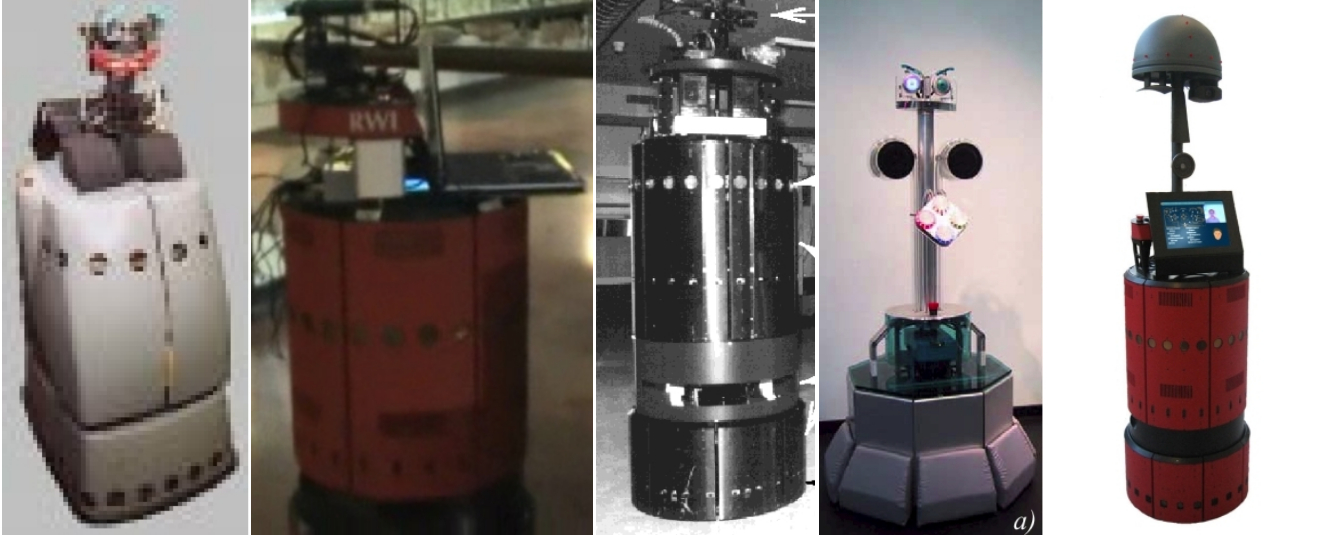
\includegraphics[width=\linewidth]{figures/minerva_cice_rhino_robox_rackham.jpg}
	\caption{Some robots that have been deployed in the real world. From the left to right: Minerva, CiceRobot, Rhino, Robox and Rackham.}
\end{figure}

Other than guiding people in museums and exhibitions, mobile robots have also been deployed in the field of healthcare: \cite{pearl_pollack_2002}, \cite{kim_socially_2016}, and \cite{kuderer_feature-based_nodate} and shopping malls: Shopbot \cite{shopbot_kanada} and Toomas \cite{toomas_gross_2009} who provided interactive support and guidance to people. 

%With some of the more recent works done by Kim and Pineau and Kretzschmar et al take a different approach. Instead of working with helper robots to guide others, the choose robotic wheelchairs as their platform to help disabled individuals navigate through human crowds. \\

%Today, we are surrounded by machines of varying complexity, competence, and autonomy, all with the common goal of making human life easier. Some common use cases include but are not limited to: giving museum tours, guiding people at the airport, assisting the elderly and needful.   \\

Navigation is one of the fundamental problems in the field of mobile robotics with decades of research flowing into it. In its simplest form, it can be defined as a process that enables a robot to move from its current position (stating position) to a desired position( goal position) avoiding collisions along the way. Work on artificial potential field by O.Khatib \cite{khatib_1986} and various flavors of graph-based search algorithms address this problem. \edited{In terms of deployment in the real world, Shakey Project \cite{project-shakey} was among the first to introduce a robot with capabilities to successfully perceive and navigate its surroundings.}\\

Deploying mobile robots in the presence of humans introduces a new set of challenges. Avoiding collisions and reaching a given destination are no longer sufficient, now these must be achieved in a 'socially acceptable' manner. The \edited{subjective} nature of this additional objective of being socially acceptable makes the problem \edited{especially} challenging. This is primarily because there is no strict definition of 'socially acceptable', and is highly dependent on the socio-cultural background of the people in the crowd and the situation at hand. This warrants and subsequently has led to research specifically geared towards socially compliant navigation.\\

\thcomment{"Even though navigation is a basic robot skill, the robotics and HRI communities have not yet produced
	a holistic approach to human-aware navigation. However, pioneering works on several individual aspects
	of human-aware navigation exist. This paper introduces human-aware navigation as a research topic and
	provides an overview of the existing research, including not only navigation techniques, but also evaluation
	methods." - \cite{kruse_human-aware_2013}\\ Can I use this to cite for the statement "This warrants and subsequently has led to research specifically geared towards socially compliant navigation."}

\edited{Kruse et. al. \cite{kruse_human-aware_2013} identify 3 broad areas of focus in the existing literature that make a robot more acceptable in a social context, which leads to improvement in $3$ qualitative attributes:}

\thcomment{ From what I have found so far, \cite{kruse_human-aware_2013} is one of the most cited survey paper on this topic in recent times.}
\begin{enumerate}
    \item \textbf{Comfort}: how comfortable people are around a robot. 
    \item \textbf{Naturalness}: how natural the movement of a robot is. This is synonymous with the predictability and interpretability of the robot's movements.
    \item \textbf{Sociability}: respecting cultural norms like preferring the right side of a hallway and, not cutting through a group of people: to name a few. %These fall into the category of what we like to call 'common courtesy'
\end{enumerate}

\subsubsection{Work on comfort}
Addressing the aspect of comfort has been one of the more researched areas in the field of social navigation \cite{kruse_human-aware_2013}.\\

\thcomment{"Research on human-aware robot navigation follows different goal: \textbf{Most of the papers we collected attempted to minimize annoyance and stress, thus making interaction more comfortable for the human.} Others
	strive to make robots behave more natural within their abilities or make robots behave according to cultural
	norms. All three goals have in common that they attempt to improve robot acceptance, but the methods
	vary. These terms like "comfort" and "natural" are used loosely in literature, so in order to classify the
	papers, we use the following definitions." - \cite{kruse_human-aware_2013}}

 Relative distance from a person has been the primary gauge to measure comfort. These are largely based on the work of Edward T. Hall in proxemics \cite{proxemics_hall_1968}. Proxemics deals with the study of personal territory. While this is dependent on the socio-cultural background of an individual, and the context of the scene, Hall divides the personal territory into 4 \edited{zones}: public, social, personal, and intimate, each reserved for a different purpose as described in \autoref{tab:proxemics}
\begin{table}
    \begin{center}
        \renewcommand{\arraystretch}{1.3}
        \begin{tabular}{|p{0.2\textwidth}|p{0.15\textwidth}|p{.57\textwidth}|}
            \hline
            Name of zone & Distance & Use case \\
            \hline\hline
            Intimate space & 0 - 45cm &  Interacting with close friends and intimates. Generally involving physical contact.\\
            Personal space & 45 -120cm &  For interaction with close friends and family. \\
            Social space & 1.2 - 3.6m &  Interacting with acquaintances and people one is familiar with.\\
            Public space & > 3.6m &  Interacting with a crowd of people.\\
            \hline
        \end{tabular}
        \caption{Categorization of Proxemic distances.}
        \label{tab:proxemics}
    \end{center}
\end{table}
Other work exploring the comfort aspect of human-robot communication focuses on specific cases like:
\begin{enumerate}
    \item \textbf{Approaching a person:} Dautenhahn et al. \cite{dautenhahn_2006}  study different ways to approach people who are seated. They find that the best way is to approach from the side and not from the front.
    [Koay et al. \cite{koay2007ExploratorySO}  found that $58\%$ of participants preferred a frontal approach by the robot while $75\%$ preferred a frontal approach when the robot was handing them something.
    \item \textbf{Passing a person:} [Pacchierotti et al. \cite{pacchierotti_2006} \cite{pacchierotti_2005},  show that proper signaling while approaching a person and maintaining a healthy distance is a desired trait in a mobile robot.
    \item \textbf{Moving in the vicinity of a person:}  Butler et al. \cite{butler_2001} test on different approaching speeds, trajectories taken by a robot to avoid a person and exploratory movements of robots in general and find that in general people prefer slower speed, and greater gap maintained by a robot passing by.
\end{enumerate}

\edited{A majority of the existing work, that aim to increase comfort, design cost-maps based on the findings of the aforementioned studies.} These produce navigating agents that maintain a healthy distance from nearby people. Some aim to reduce the surprise factor in their robot navigation by structuring penalty functions that emphasize motion in the field of view of nearby people \cite{pandey_2010_human_centered_nav}, \cite{scandolo_2011}, \cite{sisbot_human_2007}.
Others concentrate on specific scenarios like approaching, tracking, and following people.\\

Recent works using reinforcement learning algorithms also fall into this category. They primarily focus on two things: the structure of the reward, and the representation of the environment. \\

Rewards are engineered focusing on collision avoidance and maintaining proxemics distances from nearby pedestrians \cite{chen_crowd_aware_robot_nav_with_attention}, \cite{chen_decentralized_non_communication_2017}. Other works incorporate a more intricately designed reward function that captures rudimentary social norms like overtaking from the left,  and passing from the right \cite{chen_socially_2017}. \\
\thcomment{\cite{chen_socially_2017} is a work on robots interacting with pedestrians. I am guessing people follow similar rules while walking?}

\edited{Reinforcement learning algorithms base their decisions on observations from the environment. A key component of these methods is the precise interpretation and proper representation of its nearby surroundings to generate meaningful observations. Long et al. \cite{long_2017_optimally_decentralized_collision_avoidance} and Tai et al. , \cite{tai_paolo_virtual_to_real_2017} work with raw observations from the environment. Chen et al. use pairwise interaction \cite{chen_crowd_aware_robot_nav_with_attention}, \cite{chen_decentralized_non_communication_2017} between a robot and the pedestrians nearby, modeling human-human interaction using local maps \cite{chen_crowd_aware_robot_nav_with_attention}, and pooling information using attention-based mechanisms \cite{chen_crowd_aware_robot_nav_with_attention}.}

\subsubsection{Work on naturalness}
\edited{While comfort is necessary, it is not sufficient.} Naturalness in the motion of the robot and the trajectory it traces play an important role in the social acceptance of a robot. \\
\thcomment{This is all I have regarding this : "Several publications attempt to make robots navigate more acceptably near humans by making robots
	move more similar to how humans move. This is often called "natural" behavior. The assumption is that if a
	robot behaves like a human (or like an animal), the interaction between humans and the robot becomes easier
	and more intuitive for the humans. Related adjectives are "predictable", "understandable", "readable" or
	"legible". All those concepts rely on the fact that robot motion is interpreted by human observers, who
	attempt to judge the motive and the future behavior of the robot. As an example this is necessary as a
	human might need to proactively interrupt the robot if the safety of the human, the robot or the environment
	are at risk. The likelihood that a human observer interprets the motion of the robot correctly is assumed
	to be higher if the robot moves naturally." - \cite{kruse_human-aware_2013}. So, I think it is more of an assumption than hard evidence.}
\\Work falling under this category deal with the motion of the robot, rather than its effect on its surrounding and attempts to improve its predictability and interpretability.\\ %If a human being sees the robot, he/she would be able to understand/interpret its intentions and the trajectories taken by the robot would somewhat be similar to that of a person put in a similar context. 
Factors that help perceive a mobile robot as natural include:
\begin{enumerate}
    \item \textbf{Smooth motion:} Humans prefer a gradual, consistent change in orientation and velocity. This traces smooth paths that optimize for the energy spent in the execution of the trajectory \cite{arechavaleta_nonholonomic_2008}. Sudden changes in orientation and speed while moving in a crowd makes a robot unpredictable and thus seem unnatural. \cite{pandey_alami_robot_guide_2009, pandey_2010_human_centered_nav} work on smoothing trajectories.
    \item \textbf{Natural interaction:} A large portion of the time we spend during navigation in groups involves interaction with others. Some of the traits we commonly exhibit that has been the focus of research are following people moving in the general desired direction \cite{gockley_natural_person_following_2007}, maintaining a formation while interacting with nearby people \cite{althaus_nav_for_human_robot_interaction_2004}, and non-verbal communication with people nearby \cite{sauliner_minimal_nonverbal_interruption_2011}. 
    
\end{enumerate}
\thcomment{Figure for the above if possible}
\subsubsection{Work on sociability}
Social and cultural norms are the collection of explicit and tacit rules that we as a member of the society agree up to maintain harmony. Examples of this would include but not limited to waiting in a queue, preferring a particular side of a pathway, and waiting for people to exit an elevator before entering. While the presence of these traits is not vital, the lack of adherence to social norms can cause discomfort and evoke mistrust among people nearby. Some of the work in the existing literature addresses a few of these problems. Kirby et al. \cite{kriby_companion_2009} encodes within their cost function the preference for the right side of a corridor. \cite{pandey_alami_robot_guide_2009} make the robot overtake a pedestrian from the right.\\

While most of the approaches produce reliable controllers on and off the simulator, they optimize for a set of goals that are geared towards optimizing for navigation using a smartly engineered reward function which in turn relies on proxemic distances and in some cases a few of the obvious social norms.\\

\section{Inverse reinforcement learning in social navigation}
One of the primary issues associated with formulating a reward function for social navigation is the vast variety and elusiveness of the 'social rules'. \edited{Inverse reinforcement learning (IRL) or inverse optimal control is a class of methods} put forward by Russell \cite{russel_irl_1998} that seek to address this issue. The goal of IRL is to obtain an optimal controller that performs like an expert and in the process recover the underlying reward function using demonstrations from the expert. \\

Abbeel and Ng \cite{abbeel_apprenticeshiplearning_2004} show that matching the feature expectation of the agent to that of the expert translates to a similarity in their performance in the context of a Markov decision process(MDP). But the problem remains under constrained (ill-posed) as multiple reward functions (including degenerate ones) can lead to the expert demonstrations being optimal. Additionally, the idea of feature matching is ambiguous, as a single policy can be optimal for different reward functions and different policies can lead to similar feature expectations. \\

Ziebart et al. \cite{ziebart_maxent_2008} takes an entropy-based approach to resolve this ambiguity. They use an energy-based model where the probability of a given trajectory is proportional to the exponential of the reward it obtains. This produces stochastic policies that have equal preference over trajectories yielding similar rewards. Recent developments in IRL introduce the use of neural networks bolstering the expressive power of the reward function \cite{wulfmeier2015maximum}. \\

Due to the nature of the problem, IRL has been heavily explored in the field of social navigation \cite{kuderer_socially_nodate, kretzschmar_socially_2016}. \cite{shiarlis_rapidly_2017, okal_efcient_nodate} use IRL in conjunction with more traditional graph-based navigation methods to train agents. Here they use the IRL to infer the underlying rewards, which is then used to estimate the cost of different paths during the planning phase. \cite{kim_socially_2016} use IRL in a hierarchical navigation architecture, where they divide the task of navigation into a long term global planner based on a classical shortest-path finding algorithm, a short term controller based on IRL and a low-level collision avoidance module. \cite{kretzschmar_socially_2016} use a spline-based representation of the trajectory and use a maxent IRL formulation to train an agent using feature matching. 
\\
Both,\cite{kim_socially_2016, kretzschmar_socially_2016} implement their method on real-world robots. \cite{vasquez_inverse_2014} provide a comparative analysis of different IRL based learning algorithms and the importance of feature representation in the context of IRL. More recent works include deep learning-based methods to solve the problem of social navigation \cite{fahad_learning_2018, wulfmeier2015maximum}


In this thesis, we propose an efficient sampling-based approximation to enable model-free deep-network based inverse reinforcement learning. We also propose a goal conditioned risk-based feature representation for the social navigation problem that captures local information surrounding the agent. 

\section{Thesis outline}
The rest of the chapters of the thesis are organized as follows:
\autoref{ch:2} and \autoref{ch:3} present a detailed overview of some of the existing work in the literature based on both classical methods and data-driven approaches respectively.

\autoref{Ch:4} elaborates on the proposed navigation pipeline describing a flavor of the MEDIRL algorithm for a model-free environment along and design and the idea behind the design of the feature representation used.

We train and test our methods in an in-house built simulator, specifically designed for the task of social navigation, which is described in great detail in \autoref{ch:enviornment}

\autoref{ch:6} is the experiments section. This contains details about the different experiments conducted and how the different components of the navigation pipeline, like the feature representation and the choice of the controller algorithm, contribute to the final performance of the agent. Measuring the social compliance of an agent can be tricky. Keeping that in mind we present a set of evaluation metrics, both qualitative and quantitative which is described in this chapter.

\autoref{ch:conclusion} concludes the thesis reflecting upon the challenges faced in the task of social navigation and includes possible avenues to explore building upon the existing work.

\chapter{Literature review: Classical path planning}
\label{ch:chapter2}
\label{ch:2}
%\section{Classical methods for socially complaint navigation}

%\subsection*{Outline structure of the chapter}
%\begin{enumerate}
%    \item Describe the problem of navigation.
%    \item Describe the problem of social navigation and what how is it different from the problem of classical navigation.
%
%    \item What are the factors that make this problem hard to pin and thus hard to solve? Include works from the paper "Influence of proxemic behaviors in human-robot interaction. (Takayama et al)
%    \item Set of works done before and how they try to approach the problem.
%\end{enumerate}
%
%\subsection*{Papers to inculde}
%    \begin{enumerate}
%        \item Social forces model and its family (Reif and wang, Helbing and Molnar).
%        \item Qualitative trajectory calculus
%        \item A framework towards a socially aware mobile robot motion in a human ventured dynamic environment. - Pandey et al
%        \item Dynamic window approach for reactive collision avoidance.
%        \item Human aware mobile robot motion planner - Sisbot
%        \item Trajectory planning for robots in dynamic human environments. Svenstrup
%    \end{enumerate}
%

In this chapter, we go through some of the classical approaches from the existing literature that address the problem of socially-compliant navigation. We will start by briefly describing the method and its strengths, followed by their limitations and the subsequent body of research that improves on it.
%\subsubsection*{Khatib et al}
\par
One of the earliest path planners include A-star algorithm \cite{hart1968} that uses a graph-based heuristic search to determine the path with the least cost between two points. More recent work on controllers for autonomous navigation is based on artificial potential fields \cite{khatib_1986}. The main idea behind the method is that an agent moving through a scene is analogous to a particle moving through a force-field, where the goal exerts an attractive force while the obstacle surfaces negative forces. The resultant force, which is inversely proportional to the distance between these external entities, then guides the agent towards the goal while avoiding incoming obstacles as shown in \autoref{fig:artificial_pf}. The resulting controller, with proper hyper-parameters, does a fairly good job of navigating a scene checking all the boxes of a good navigating agent: it reaches the goal location avoiding obstacles along the way. There are many drawbacks to this method. The most notable being getting stuck in local minima, which were addressed by more sophisticated methods like probabilistic road-map based approaches \cite{Lavalle98rrt}. \\
%\subsubsection*{Helbing and Molnar: Social Forces}
\begin{figure}
	\centering
	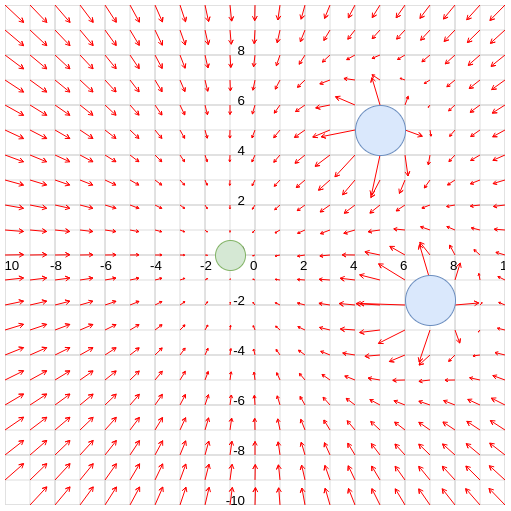
\includegraphics[width=\linewidth]{figures/vector_field_pf.png}
	\caption{Graphical representation of an artificial potential field. The force field guiding any agent  towards the goal at (-1, 0) (green circle) is disrupted by the repulsive forces of the obstacles located at (5,5) and (7, -2))}
	\label{fig:artificial_pf}
\end{figure}
Building on artificial potential fields, Helbing and Molnar introduce a pedestrian model that follows principles similar to that of the artificial potential fields and encapsulates a richer set of information to imbibe `social' behavior in the agent's movement \cite{helbing_social_1998}. Rather than representing the force applied to an agent as the sum of the forces from external factors (obstacles and goal(s)), they model the pedestrian behavior as a combination of a set of internal motivations.\\
%\thcomment{Here "they refers to the work of Helbing and Molnar. Should I change the wording?}

The formulation is given by:
\\
%\thcomment{\cite{helbing_social_1998} in their paper had a bunch of equations describing the different forces acting on the agent, the sum of which is given by the equation \autoref{eq:helbing_final_eq}. I get it. Here, writing 'final' is out of context.}
\begin{align}
\label{eq:helbing_final_eq}
\frac{d\vec{w_{\alpha}}}{dt}:=\vec{F_{\alpha}}(t)+fluctuations
\end{align}
where, $\vec{w_{\alpha}}$ is the preferred velocity of pedestrian $\alpha$ and $\vec{F_{\alpha}}$ is the combined effect of all the forces acting on pedestrian $\alpha$. $\vec{F_{\alpha}}$ is further expanded as:\\
\begin{multline}
\label{eq:lebing_molnar_social_forces}
\vec{F_{\alpha}}(t):=
\vec{F_{\alpha}^{0}}(\vec{v_{\alpha}}, v_{\alpha}^{0}\vec{e_{\alpha}})+\sum_{\beta}\vec{F_{\alpha, \beta}}(\vec{e_{\alpha}}, \vec{r_{\alpha}} - \vec{r_{\beta}})
+\\\sum_{B}\vec{F_{\alpha B}}(\vec{e_{\alpha}}, \vec{r_{\alpha}} - \vec{r_{B}^{\alpha}}) + \sum_{i}\vec{F_{\alpha i}}(\vec{e_{\alpha}}, \vec{r_{\alpha}}-\vec{r_i},t)
\end{multline}
where, $\vec{r_{\alpha}}$,  $\vec{v_{\alpha}}$,  $\vec{v^{0}_{\alpha}}$ and $\vec{e_{\alpha}}$  are the current location, velocity, desired speed and desired direction of pedestrian $\alpha$. $\vec{r^{\alpha}_{B}}$ is the smallest distance between pedestrian $\alpha$ and an obstacle $B$, and, $\vec{r_i}$ is the position of any object, other than the goal, that can temporarily attract a pedestrian. \\
Each of the terms being added up in \autoref{eq:lebing_molnar_social_forces} is a mathematical formulation of an internal motivation.
$\vec{F_{\alpha}^{0}}$ is the force guiding the agent towards the goal, $\vec{F_{\alpha\beta}}$ and  $\vec{F_{\alpha B}}$ denotes the repulsive forces from other pedestrians and obstacles respectively.
$\vec{F_{\alpha i}}$  sums up the attractive forces other than the goal, that might attract a pedestrian like a street artist or a window of a shop.
\par
Careful observation and interpretation of human behavior and engineering rules that resemble them lead to the creation of a controller that provides a social flavor to the previously socially-indifferent controller obtained from artificial potential fields. Formulations of this nature are highly dependent on the different cases being considered and assumptions being made in the creation of the model.
%\textcolor{red}{A lot of careful engineering has been put into creating this 'formulae' that dictate/emulate the naturalness of human-movement while negotiating crowded space in an artificial agent/robot. 
%Formulations of this nature are highly dependent on the different cases being considered and assumptions being made in the creation of the model.}\\

%\subsubsection*{Sisbot et al}
In more recent work \cite{sisbot_human_2007}, Sisbot et al. take a similar approach, where they generate and make use of three different cost maps, $Cost_{safety}$, $Cost_{visibility}$ and $Cost_{hidden zone}$ each focusing on a separate attribute.
The $Cost_{safety}$ keeps track of how safe a location in the grid is based on the structure and kinematics of the human and his/her state, where the state includes information like the posture (sitting or standing), configuration and parameters.
$Cost_{visbility}$ is designed to penalize the robot if it is positioned outside the field-of-view of nearby pedestrians. 
The rationale being, the effort a human has to make to keep the robot in his/her vision is directly proportional to the discomfort caused by the robot with its movements. For example, regions behind a pedestrian is associated with a greater penalty as compared to regions in front.
And lastly, $Cost_{hidden zone}$ takes into account the amount of time when the robot remains hidden behind any obstacle and the penalty associated with it. 
The authors also provide two nuanced ways of merging the cost terms. One where the $Cost_{merged}$ is the weighted sum of two
\begin{align}
Cost_{merged}(x,y) = w_{1}Cost_{safety}(x,y) + w_{2}Cost_{visibility}(x,y)
\end{align}
and 
\begin{align}
Cost_{merged}(x,y) = max(Cost_{safety}(x,y), Cost_{visibility}(x,y))
\end{align}

The final cost function factoring in the $Cost_{hidden zone}$ is
\begin{align}
Cost_{final}(x,y) \leftarrow w_{3} Cost_{hidden zone}(x,y)
\end{align}
when, $x$ and $y$ are in the field of view of a human, but is obstructed by the presence of the robot and 
\begin{align}
Cost_{final}(x,y) \leftarrow Cost_{merged}(x,y)
\end{align}
Once the final cost map is obtained, a path between two points on the grid is computed using $A^*$ search. $ w_{1}$, $w_{2}$, $w_{3}$ are the weights associated with $Cost_{safety}$, $Cost_{visibility}$, $Cost_{hidden zone}$ respectively. They serve as hyper-parameters and can be tuned to meet the requirements of the task at hand.

%\subsubsection*{Svenstrup et al}
Lastly, we look into another body of work by Svenstrup et al. \cite{svenstrup_trajectory_2010}, that combines a potential field-like cost map with a probabilistic road map. Probabilistic road maps \cite{kavraki_probabilistic_1996} are a class of planning algorithms where a robot navigates from a starting point to a goal point by creating a graph in a given space. The graph is constructed by generating random samples and connecting them to the existing graph.\\
In their work, "Trajectory planning for robots in a dynamic human environment", Svenstrup et al. take on the problem of autonomous navigation in a social environment from a different direction. They use the idea of potential field combined with rapidly exploring random trees that takes into account the robot kino-dynamics while planning the trajectory.
The calculation of the potential field is broken down in three parts:
\begin{enumerate}
	\item The cost associated with the general desired behavior of the agent. The authors use a cost function with a bias towards a non-agoraphobic behavior i.e. an agent motivated not to linger at the edges of an environment. This is given by:
	\begin{align}
	g_{1}(\textbf{x}(t)) = c_{y}y^{2}(t)
	\end{align}
	where, $\textbf{x}(t)$ and $y(t)$ are the dynamical model, and position in $y$ direction of the agent at time $t$. $c_y$ is a hyper-parameter denoting the affinity of the agent to move towards the center of the environment. The dynamical model is given by \autoref{eq:robot_dynamics_sven}

	\begin{equation}
	\label{eq:robot_dynamics_sven}
	\textbf{x}(t) = 
	{%
		\vphantom{\begin{bmatrix}0\\0\\0\\0\\0\\0\end{bmatrix}}
		\begin{bmatrix}
		x_1(t)\\x_2(t)\\x_3(t)\\x_4(t)\\x_5(t)\\
		\end{bmatrix}
	}
	=
		{%
		\vphantom{\begin{bmatrix}0\\0\\0\\0\\0\end{bmatrix}}
		\begin{bmatrix}
		x(t)\\y(t)\\v(t)\\\theta(t)\\\dot{\theta}(t)
		\end{bmatrix}}	
	\rightarrow
			{%
		\vphantom{\begin{bmatrix}0\\0\\0\\0\\0\end{bmatrix}}
		\begin{bmatrix}
		\text{x position}\\\text{y position}\\\text{linear velocity}\\\text{rotation angle}\\ \text{rotational velocity}
		\end{bmatrix}}		
	\end{equation}
	The robot behavior is given by the differential equation \autoref{eq:diff_eqn_sven}
	\begin{equation}
	\label{eq:diff_eqn_sven}
	\dot{\textbf{x}}(t) = 
	\mathbf{f}(\textbf{x}(t), \mathbf{u})
	=
	{%
		\vphantom{\begin{bmatrix}0\\0\\0\\0\\0\end{bmatrix}}
		\begin{bmatrix}
		\dot{x}(t)\\\dot{y}(t)\\\dot{v}(t)\\\dot{\theta}(t)\\\ddot{\theta}(t)
		\end{bmatrix}}	
	\rightarrow
	{%
		\vphantom{\begin{bmatrix}0\\0\\0\\0\\0\end{bmatrix}}
		\begin{bmatrix}
		x_3(t)\cos{x_4(t)}\\	x_3(t)\sin{x_4(t)}\\u_v(t)\\ \dot{\theta}(t) \\ u_\theta(t)
		\end{bmatrix}}		
	\end{equation}
	where, $u_v$ is the linear acceleration and $u_\theta$ is the rotational acceleration.
	\item The cost associated with the presence of humans in the vicinity. This is based on their previous work, "Pose Estimation and Adaptive Robot Behavior for Human-Robot Interaction" \cite{svenstrup_pose_estimation_2009}, where a potential field is constructed by fine-tuning the co-variances of four Gaussian distributions expressing the following information: attraction towards a human, preventing the robot to approach a human from behind and two distributions to account for the parallel and perpendicular direction to the Person Interest indicator, which is calculated based on the person's velocity, position and pose.  
	\begin{align}
	g_{2}(\textbf{x}_{1:2}) = \sum_{k=1}^{4}c_{k}\exp(-\frac{1}{2}[\textbf{x}_{1:2} - P_0]^{T}\sum^{-1}_{k}[\textbf{x}_{1:2} - P_0])
	\end{align} 
	where $c_{k}$ are the normalizing constants, $\textbf{x}_{1:2}$ denote the first two components of the robot dynamics, $P_0$ is the position of the person, and $\sum_k$ are the co-variances of the Gaussian distributions.
	\item The cost associated with the goal that penalizes the robot for not moving or not orienting itself towards the goal. The cost is not uniform and is skewed to have a higher penalty at shorter distances.
	\begin{align}
	g_{3}(\textbf{x}(t)) = c_{e1}\exp(c_{e2}(x(t) - \hat{x}(0))) + c_{\theta}\theta^{4}(t)
	\end{align}
	where, $c_{(.)}$ are constants, $\theta(t)$ is the rotation angle at time $t$, and $\hat{x}(0)$ is the desired position at time $t=0$.
\end{enumerate}

%\textcolor{red}{Figure depicting the PF around a pedestrian?}
The final cost is given by: 
\begin{align}
G(t) = g_{1}(\textbf{x}(t)) + g_{2}(\textbf{x}(t), \mathcal{P}(t)) + g_{3}(\textbf{x}(t))
\end{align}
where, $\mathcal{P}(t)$ is the matrix containing the positions of the persons at a given time $t$ and $g_{1}$, $g_{2}$ and $g_{3}$ are the three cost functions described above.\\
The navigation is represented as a minimization problem that aims to minimize the cost of moving through the potential field while respecting the dynamic constraints of the robot and is given by:
%\thcomment{I am not sure what you wanted to convey here. Is there anything else other than making sure all the symbols are defined?}
\begin{align}
\label{eq:sven_optimziation}
\begin{split}
minimize \qquad I(\tilde{u}_{0:T}) = &\int_{0}^{T} [g_{1}(\textbf{x}(t)) + g_{2}(\textbf{x}(t), \mathcal{P}(t))]dt + g_{3}(\textbf{x}(t))\\
s.t. \qquad \qquad \dot{\textbf{x}}(t) = & f(\textbf{x}(t),u(t)) \\
where \qquad g_{1}(\textbf{x}(t)) = &c_{y}x_{2}(t)^{2}\\
g_{2}((\textbf{x}(t)), \mathcal{P}(t)) = &\sum_{j=1}^{p} \sum_{k=1}^{4} c_{k}\exp(-\frac{1}{2}[\textbf{x}_{1:2} - \mu_{j}]^{T}\sum^{-1}_{k}[\textbf{x}_{1:2} - \mu_{j}])\\
g_{3}(x(T)) = & c_{e1}\exp(c_{e2}(x_{1}(T) - x_{1}(0))) + c_{\theta}x_{4}^{4}(T)
\end{split}
\end{align}
where $\tilde{u}_{0:T}$ is the input sequence to the robot from time $t=0$ to $t=T$, $\mathcal{P}(t)$ is the position and orientation of the present people at time $t$, $\mu_{j}$ is the position of the pedestrian, $j$.\\

The choice of trajectory planner used for the problem at hand is a modified rapidly exploring random tree (RRT). They introduce a step to prune the nodes that helps in reducing the size of the tree and improving the stopping condition for extending the tree. Instead of depending on an error, they place a limit on the number of nodes that can be added to the tree and terminate accordingly. %\thcomment{The following line is one of the steps in their algorithm. not an explanation of the of the expression above. I did not make any changes to address your comment. }
 Finally, the trajectories with a smaller penalty are preferred over trajectories with newer vertices.

\par
%\textbf{Their overall algorithm:????}
%%%%% conculsion %%%%%%
A theme for most of the model-based approaches to the path planning problem is two fold: design a cost function that takes into account a set of social norms and construct a navigation model based on it.\\
While this approach has been tried, tested, and shown to be capable of navigating in the presence of humans, there are a few drawbacks. The design of the cost functions is highly dependent on the particular social etiquette and cultural norms that had been considered at the time of designing the model. There are many social conventions and tacit agreements that we as humans follow and respect while navigation, like not obstructing people engaged in a conversation, or, respecting personal space when possible, to name a few. The full set is hard to enumerate and never explicit making it difficult to take into consideration in the design of the model. Some of the issues arising from the model-based approach can be circumvented by using a data-driven approach as elaborated in \autoref{ch:3}.













\chapter{Literature review: Data driven approach}
\label{ch:chapter3}
\label{ch:3}
In this section, we discuss different learning-based approaches that have been explored in recent years. Learning-based methods in the field of social navigation can be broadly classified into reinforcement learning (RL)-based and inverse reinforcement learning(IRL)-based approaches. While these methods differ at their core, the problem definition for both the cases is mostly similar but with a key difference. For both RL and IRL setting, the problem at hand is expressed in the form of a Markov decision process (MDP). We define the problem below.
\subsection*{Problem definition:}
A Markov decision process is a discrete-time stochastic control process and can be represented as a 5 tuple
($\mathcal{S}$,$\mathcal{A}$,T,$\gamma$, $\mathcal{R}$), where,
\begin{itemize}
    \item $\mathcal{S}$ is the set of all possible states.
    \item $\mathcal{A}$ is the set of all possible actions.
    \item T is the transition dynamics.
    \item $\gamma$ is the discount factor.
    \item $\mathcal{R}$ is the set of rewards.
\end{itemize}  
In reinforcement learning problems, the goal is to find a policy $\pi$: a function that maps a state to an action that maximizes the expected reward obtained.\\
In contrast, in inverse reinforcement learning problems, there is no reward function. Instead, a set of expert demonstrations is provided. This can be denoted by, D = \{$\tau_1$, $\tau_2$, ... \}. The goal is to generate a reward function $\mathcal{R}$, which best explains the expert behavior and a policy that maximizes the reward function.


\section{RL based approaches}
 With their remarkable success in the field of video games and a suite of tasks of similar anatomy, RL has been one of the go-to tools in the field of social navigation in recent years. \\
Chen et al. \cite{chen_socially_2017} address this problem by focusing on what not to do, rather than what to do. They introduce a reward function crafted to induce social norms in the behavior of the agent. The reward function primarily focuses on three different aspects of interaction: overtaking, passing, and crossing as shown in the figure below.
 \begin{figure}[!htbp]
     \centering
    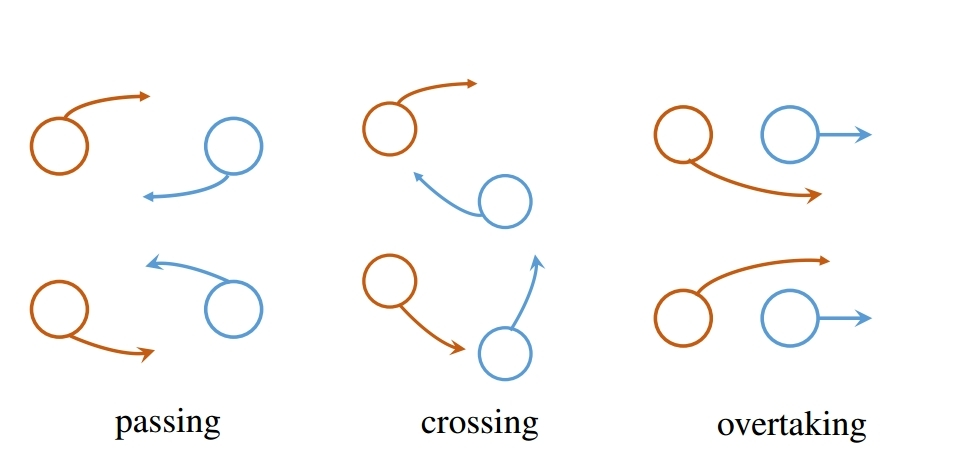
\includegraphics[width=.6\linewidth]{figures/chapter2_rl_based_approach}
    \caption{Representation of the three interaction scenarios.}
    \label{fig:label1}
 \end{figure}
\\
They note that symmetry is one of the driving factors to incorporate social behavior, so they introduce a network architecture for symmetric multi-agent training.\\

A more recent work by the same authors, Collision avoidance in pedestrian-rich environments with deep reinforcement learning \cite{everett_collision_2019}, 
address drawbacks of their previous work: the inability to tackle a variable number of agents in the environment. They introduce a Long Short-Term Memory (LSTM) \cite{hochreiterLongShortTermMemory1997} based network architecture that takes as input the information from the nearby pedestrians in a sequence. This eliminates the need for specifying a limit on the number of nearby-agents the method can handle.\\
The state comprises of two parts: 
\begin{enumerate}
    \item The information of the agent itself, \textbf{s}
    \item The information from the other $n$ number of agents present in the environment at a given time. This is where the LSTM comes in to play and takes information from these n agents and passes them sequentially through an LSTM layer to generate a final hidden state which is concatenated with \textbf{s} to obtain the final state representation of the environment.
\end{enumerate}
\begin{figure}[!htbp]
    \centering
    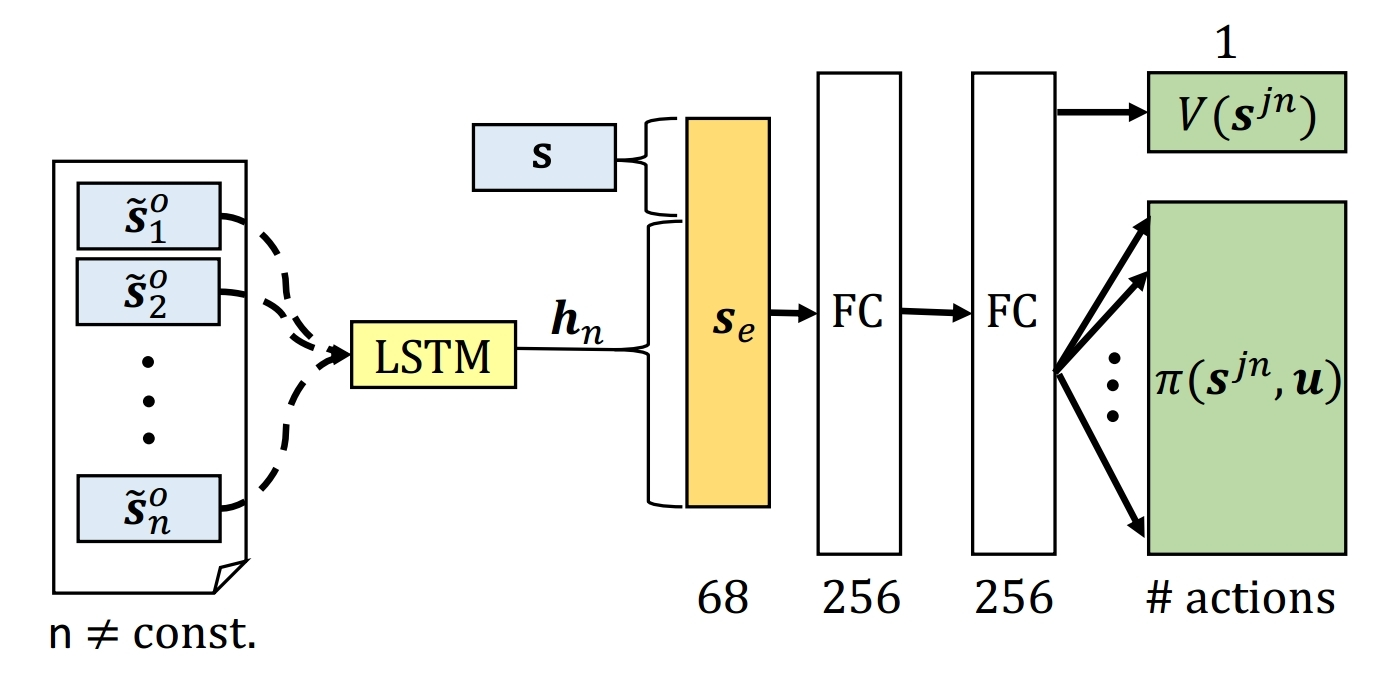
\includegraphics[width=0.6\linewidth]{figures/everett}
    \caption{LSTM based network architecture to account for a variable number of nearby agents.}
    \label{fig:label2}
\end{figure}

The reward function used in this work is a relatively straight forward and sparse with positive and negative feedback for either reaching the goal and encountering a collision respectively.

%\textbf{Conclusion}\\
Reinforcement learning, as a class of methods, has been widely successful in solving various complex control tasks including but not limited to video games making it one of the more preferred choices to tackle the problem of social navigation. \par
However, using RL in this particular setting necessitates the formulation of a reward function that can correctly capture the 'social and cultural' characteristics. Coming up with such a set of rules can be difficult and daunting as 'social norms' are not always explicit and can vary widely across different societies and even based on a given situation.\\

\section{IRL based approaches}
%\textbf{Learning approaches meet probabilistic road map style path planner.}
Engineering a reward function that illicit social compliance from an agent is difficult. That is why a lot of the recent research in this field takes the approach of inverse reinforcement learning. \par 
Vasquez et al. in their work \cite{vasquez_inverse_2014}, present a comprehensive study on the effect of different feature representations and IRL methods on the performance of an agent in the task of social navigation. They examine two IRL methods: max-margin IRL and max entropy IRL.\\
For the feature representations, they create a pool of measurements garnered from the state of the agent itself and the state of the other entities in the environment and combine these measurements to create 3 feature representations. \\
They test all of these on a ROS based pedestrian simulator on 3 scenarios: airport gate, crossing hallway, and intersection. Expert demonstrations for these scenarios are obtained through teleoperation. They find that the performance across the two learning methods are similar. The feature representation, on the other hand, plays a major role in the final performance of the agent hence they come to the conclusion that spending time on modeling the feature representations or working to come up with learning methods that aid in the simplification of building the feature representations might be the way to go.
\\
\par
Kim and Pineau in their work \cite{kim_socially_2016}, Socially adaptive path planning, present a way to automate the navigation of a wheelchair in a social setting. Their navigation framework comprises of 3 components, the feature extractor, the IRL module, and the path planner.\\
%\textbf{Feature extractor}
The features are generated from the readings of an RGB-d sensor ($3$D point cloud) mounted on the robot. The area around the agent is divided into $3$D blocks or cells and the features are calculated for each of these spatial cells. 
The authors calculate $4$ features namely,
crowd density, speed, velocity, and distance to the goal.
While the calculation of the crowd density and the distance to the goal is straight forward, the calculation of the speed and velocity from 3d point clouds are more involved and the authors use an RGB-d optical flow method based on Farneback RGB optical flow \cite{farneback_optical_flow}. 
The result is a $12$-dimensional binary feature vector for each grid cell.
%\textbf{IRL module}
The authors use Maximum a posterior i Bayesian Inverse reinforcement learning (MAP-BIRL) \cite{choi_MAP-BIRL_2011} to calculate the cost function for socially acceptable navigation. Cost of a state is given by
\begin{align}
C(s,a) = \sum^{d}_{i=1} w_i \phi_i(s,a)
\end{align}
where the weight vector w is learned from MAP-BIRL. 
The weight vector is obtained by obtaining the MAP inference of the following expression:
\begin{align}
L(w) = \sum^M_{m=1} \sum^{H}_{h=1}log[\frac{\exp \mathcal{Q}^{*}_m(s^m_h, a^m_h)}{\sum_{a\in A} \exp(\mathcal{Q}_m^*(s_h^m,a))}]
\end{align}
For path planning, the authors maintain a hierarchical path planner consisting of 3 parts: global planner, local planner, and a collision detector.
The global planner chalks out a global path from the starting position of the robot to the goal state. The entire path is broken down into multiple sub-goals and the responsibility of moving from one sub-goal to the next falls on the local planner. During the run, the planner maintains a collision detector based on handcrafted rules.
The authors test their method on different scenarios including one that involves the robot operating in a crowded corridor.\\

Fahad et. al. \cite{fahad_learning_2018}, present a navigation framework to train agents from demonstrations using maximum entropy Deep IRL where the objective is to maximize the likelihood of the states visited by the expert.
This is achieved by dividing each demonstration, or trajectory, in this case, into a sum of the individual states encountered by the expert. and minimizing the difference in the state visitation frequency (SVF) of the agent and the expert.\\
The authors present a feature representation consisting of 4 parts:
\begin{enumerate}
    \item Social Affinity Map(SAM): This captures the motion of the pedestrians in the vicinity of the agent. The area near the agent is divided into two concentric circles. The region inside the inner circle is then divided into 4 parts, and the region between the inner and outer circle is divided into 6 parts.
    Information from each of these 10 areas (or bins) is then expressed using a 6-dimensional vector that captures the average velocity of the pedestrians in a given bin. 
    \item Density feature: Helps provide an idea of how dense the vicinity of the agent is. It is calculated by adding up the number of pedestrians present in the spatial bins (calculated above). Once calculated they are discretized based on some predefined threshold.
    \item Distance feature: Captures the distance between the agent's current location and the goal.
    \item Default Cost feature: Introduced to balance the rest of the other features. This has been proposed by various other works in the past.
    
\end{enumerate}
The authors train and test their procedure using data collected in the "ATC" business center in Osaka, Japan.
From these experiments, they show that the method is not only capable of producing a general navigator to negotiate the crowd, but also an agent that show traits of pedestrian behaviors like collision-avoidance and following the leader.

Given the nature of the task, IRL based methods seem to be a promising avenue to explore. But the problem of social navigation is far from solved and many issues still need addressing. IRL methods are highly dependent on the design of the feature representation used in the algorithm, and a lot of time and effort are needed towards optimizing a set of features that would perform well. Moreover, for most of the existing work, not a lot has been discussed about the generalization of the agent. Most of the experiments are either conducted in a relatively simple environment, like a narrow hallway, or address some specific aspect of crowd navigation like negotiating intersections. 
\begin{comment}
\textbf{Collection of expert trajectory might be expensive}
\textbf{The generalization of the method is not that great for now}
\textbf{The dependence of IRL on feature engineering: IRL methods are highly dependent on the design of the feature representation used in the algorithm, and a lot of time and effort are needed towards optimizing a set of features that would perform well.}

The primary advantage of IRL over the other methods discussed, both model-based and data-driven methods, is that there is no need to specify a handcrafted reward function built to induce certain kinds of behavior within the agent. Most of the current work in this domain primarily focuses on capturing the expert's behavior, thus encapsulating the 'naturalness' in the movements during navigation.
Disadvantages:
Comment of IRL and feature engineering. 
Getting expert demonstrations are more expensive compared to RL.
Hard to generalize. 
\end{comment}

\chapter{Design and Methodology}
\label{ch:chapter4}
\label{Ch:4}
In this section, we describe our data-driven inverse reinforcement learning based social navigation pipeline.\\
%\\ \textbf{An image showing the block diagram of the pipeline including the environment, the feature extractor, and the other components}

\begin{figure}[!htbp]
	\centering
	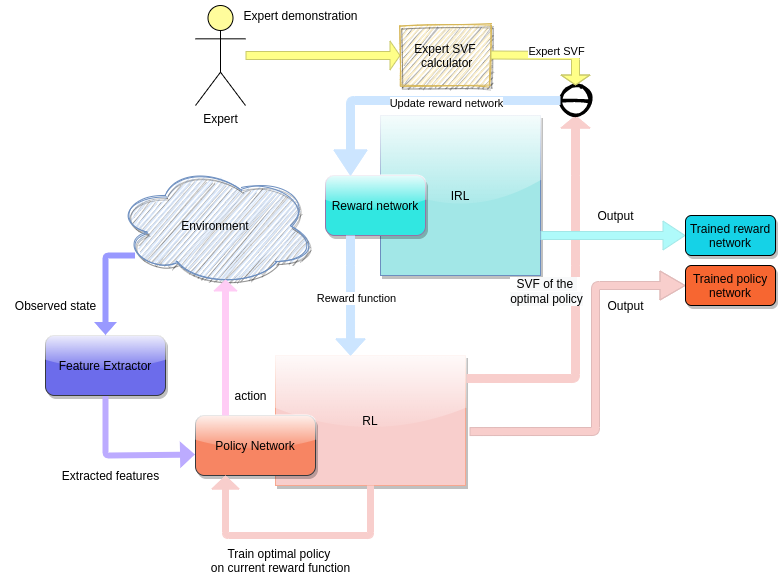
\includegraphics[width=\linewidth]{figures/irl_pipeline.png}
	\caption{An overview of the proposed navigation pipeline. The feature extractor filters data from the environment before relaying it into the RL module. Using the reward network, the RL algorithm trains an optimal policy. The difference between the state visitation frequency of the optimal policy and that of the expert is then utilized to update the parameters of the reward network. On completion, we obtain a reward function and an optimal policy corresponding to that reward function.}
	\label{fig:irl_pipeline}
\end{figure}

\section{The IRL block:}
Inverse reinforcement learning(IRL) or inverse optimal control (IOC) has been extensively explored to train robots in real-world tasks. The appeal of IRL is that it removes the need to manually construct a reward function that dictates the optimal behavior of an agent. Instead, a reward function that induces the desired behavior can be recovered from a set of expert demonstrations which is more readily available compared to an artificially constructed reward structure as needed in reinforcement learning (RL).

To keep the chapter self-contained, we will briefly recap our definition of a Markov decision process (MDP):
A Markov decision process or MDP can be defined as a tuple ($\mathcal{S}$,$\mathcal{A}$,T,$\gamma$, $\mathcal{R}$)  where,
\begin{itemize}
    \item $\mathcal{S}$ is the set of all possible states.
    \item $\mathcal{A}$ is the set of all possible actions.
    \item T is the state transition dynamics, i.e. the probability of moving to a state given its previous state and action, $P(s^{'}|s, a)$.
    \item $\gamma$ is the discounting factor.
    \item $\mathcal{R}$ is the set of rewards $R:  \mathbf{f}_{s} \mapsto \mathbb{R} $ is the reward function, where $\mathbf{f_{s}}$ is the feature vector obtained from state $s \in \mathcal{S}$.
    \begin{align}
    \phi(s) &= \mathbf{f}_{s} \\
    \mathbf{f}_{\tau} &= \sum_{s \in \tau} \mathbf{f}_{s}
    \end{align}
    where $\phi(.)$ is the feature extractor function used, and $\mathbf{f}_{\tau}$ is the feature vector corresponding to a given trajectory $\tau$ 
    \end{itemize}  
The goal of IRL is to infer a reward function that maximizes the likelihood of the expert behavior. The expert behavior is represented in terms of expert demonstrations or trajectories, $\mathbf{D} = \{ \tau_1, \tau_2, \tau_3, \dots, 
\tau_{M} \}$ in the context of navigation. Each of these trajectories, in turn, can be further broken down into a collection of states $\tau_{i} = \{ s_{0}, s_{1}, s_{2}, \dots, s_{T} \}$ as visited by the expert in the trajectory. \\ Abbeel and Ng
\cite{abbeel_apprenticeshiplearning_2004} shows that solving the Bellman equations for an analytic solution to obtain the reward $\mathcal{R}$ is under-constrained. Ziebart et al. \cite{ziebart_maxent_2008} addresses this by introducing an entropy-based constraint \cite{jaynes1957information} on the distribution of the trajectories which state that the probability of the occurrence of a trajectory is directly proportional to the reward it receives which is equal to the summation over the reward it receives at each state in the trajectory.
\begin{align}
P(\tau_{i}| \theta) = \frac{1}{Z(\theta)}\exp^{\theta^{T}\mathbf{f}_{\tau_{i}}} = \frac{1}{Z(\theta)}\exp^{\sum_{s_{j}\in\tau_{i}}\theta^{T}\mathbf{f}_{s_{j}}}
\end{align}
\begin{align}
Z = \sum_{\tau_{i}\in \mathbf{D}}\exp{\theta^{T}\mathbf{f}_{\tau_{i}}}
\end{align}
where, $Z$ is the normalizing term, $\theta$ are the weights of the reward function, and $\mathbf{D}$ is the set of all possible trajectories.\\
Given a set of expert demonstrations, an optimal reward structure should maximize the probability of the occurrence of the expert demonstrations and their associated states. Mathematically, this is given by: 
\begin{align}
\label{eq:loglikelihood-IRL}
\theta^{*} = \argmax_{\theta} \mathbf{L}(\theta) = \argmax_{\theta} \sum_{\tau \in D} \log{P(\tau| \theta, T)}
\end{align}
Ziebart et al. \cite{ziebart_maxent_2008} uses a linear combination of weights which lacked the ability to capture complex non-linear reward functions. This drawback was alleviated by Wulfmeier et al. where they restructure the maximum entropy IRL formulation using neural networks \cite{wulfmeier2015maximum}. Neural networks are universal function approximators. This vastly increases the amount of complexity a reward function can express.\\
The parameters of the reward network, $\mathbf{R}_{\theta}$ represented by $\theta$ can be found using gradient descent methods. The  update term for the reward network parameters w.r.t. the loss term $\mathbf{L}$ is equal to the difference in the state visitation frequencies (SVF) of the expert demonstrations and the optimal policy $\pi_{\psi} : \eta(s) \mapsto \mathcal{A} $, trained on the parameters of the current reward network $R_{\theta}$:
\begin{align}
	\label{eq:IRL-parameter-update-states}
	\frac{\partial \mathbf{L}}{\partial \theta} = \left(\sum_{\tau_{i} \in D}\sum_{s_{j} \in \tau{i}}s_{j} - \sum_{\hat{\tau} \in \hat{D}}\sum_{s_{k} \in \hat{\tau}}s_{k}\right)
\end{align}
where, $\hat{\tau}$ is a trajectory sampled by the policy $\pi_{\psi}$.\\
Replacing a state, $s_{i}$, by its features, $\phi(s_{i})$, \autoref{eq:IRL-parameter-update-states} can be re-written as:
\begin{align}
	\label{eq:IRL-parameter-update-features}
	\frac{\partial \mathbf{L}}{\partial \theta} = \left(\expectval_{s \sim P(s|\mathcal{D})} \phi(s) - \expectval_{s \sim P(s|\pi_\psi)} \phi(s)\right) \frac{\partial R_\theta}{\partial \theta} 
\end{align}
where, $P(s|\mathcal{D})$ and $P(s|\pi_{\psi})$ are the probability of occurrence of state $s$ following the expert demonstrations $\mathcal{D}$ and policy $\pi_{\psi}$ respectively.
%\thcomment{All the symbols have been defined before. Do I still need to redefine them after each equation?}
\subsection{The SVF calculation}
One of the main challenges of IRL is calculating the expected state distribution or the state visitation frequency (SVF) of a policy $\pi_{\psi}$. The SVF is calculated over all possible trajectories, which is computationally expensive for environments with large but finite state-spaces and intractable for continuous state-spaces. In model-based environments with finite state-space, this can be calculated using the state transition matrix and dynamic programming \cite{wulfmeier2015maximum}. Access to the underlying state-dynamics of an environment, especially in real-world applications like navigation, is difficult and not readily available. Instead, we relax this by assuming a model-free but deterministic environment.\\
%\edited{This is a reasonable assumption in the context of a navigation robot because the movements of an agent given a control command are inherently deterministic.}
%\thcomment{The reason the environment is deterministic is because the movement of the other pedestrians in the environment are dictated by an annotation-file (as they are data from a real video), which is deterministic. I am finding it hard to reason for why a deterministic environment other that the aforementioned fact. Should I just state this?} 
%This is a reasonable assumption in the context of a navigation problem because the movements of pedestrians, in general, are inherently deterministic. %and any observed uncertainty by the agent can be attributed to the error in measurement by the onboard sensors.\\

We use sampling to get an estimate of the SVF. While this can be time-consuming and computationally expensive, the task is drastically simplified when using greedy policies, especially in a deterministic environment. SVF calculation of a greedy policy in a deterministic environment can be calculated by taking a single sample trajectory (due to the deterministic nature of the environment) for each pedestrian by replacing them with the agent and letting it run till completion. The calculation of the expected state visitation frequency of the agent is shown in equation \autoref{eq:svf-sampling}

\begin{align}
\label{eq:svf-sampling}
   \expectval_{s \sim P(s|\pi_\psi)} \phi(s) \approx \sum_{s_0 \in p_0} \sum_{t=0}^{T} \phi(\hat{P}(s_{t+1}|s_t, a_t)\pi_\psi(a_t|s_t))
\end{align}
where, $\phi(s)$ is the features representation of state $s$, $P(s|\pi_{\psi})$ is the probability of state $s$ given policy $\pi_{psi}$, $\pi_{\psi}(a_{t}|s_{t})$ is the action taken at time $t$ in state $s_{t}$ according to the policy $\pi_{\psi}$, $s_{0}$ is the starting state, $T$ is the time horizon, and, $\hat{P}(s_{t+1}| s_{t}, a_{t})$ are the state transitions observed during the process of sampling the trajectories from the environment, and not from a known state transition model.
%The original formulation of maximum entropy deep inverse reinforcement learning (MEDIRL) is in a model-based setting and the state transition matrix is used to calculate the state visitation frequency (SVF) of the agent. While this produces an exact value of the agent's SVF, assuming the availability of the state transition matrix is fairly optimistic for most real-world tasks including navigation. In an attempt to make things less constrained we take the model-free approach and focus on calculating the SVF using a sampling-based method. 
%The SVF calculation:
%The main challenge of going model-free is the calculation of the normalizing factor(Z), which in the presence of a state transition matrix could be calculated using dynamic programming [citation of the paper]. 
%Under the assumption of a model-free but deterministic environment, the SVF of a policy can be reasonably computed by taking trajectory samples from the starting context of each of the existing pedestrians in the scene once. 
%\begin{align}
%equation 4 from iros2020
%\end{align}
%where the $\mathcal{P}$ represents state transitions obtained from sampling and not the state transition dynamics. \textbf{We argue that this assumption is reasonable in a navigation setting because the task is not inherently uncertain, and most transition dynamic uncertainty can be attributed to sensory noise and control error. We summarize our approach in algorithm 1. (Taken word-to-word from IROS manuscript)}
\begin{algorithm}[tbhp]
	\caption{Maximum Entropy Deep Deterministic IRL}
	\label{deterministic-medirl}
	
	\SetKwInOut{Input}{Input}
	\SetKwInOut{Output}{Output}
	
	\Input{$D, \gamma, p_0$}
	
	\SetKwComment{Comment}{$\triangleright$\ }{}
	\SetKwFunction{Backprop}{Backprop}
	\SetKwFunction{UpdateWeight}{UpdateWeight}
	\SetKwFunction{SolveMDP}{SolveMDP}
	\BlankLine
	$\theta, \psi \gets \theta_0, \psi_0$ \DontPrintSemicolon \Comment*[r]{Initialize parameters} 
	$\mu_e= \expectval_{s \sim D}{\phi(s)}$ \DontPrintSemicolon \Comment*[r]{Calculate expert svf}
	\For{$m \gets 1$ \KwTo M}{
		$\pi_\psi^m \gets \SolveMDP(R_\theta^m,\mathcal{S}, \mathcal{A}, \mathcal{T}, \gamma)$\\
		$\delta_{\text{svf}} = \mu_e - \expectval_{s \sim P(s|\pi_\psi^m)} \phi(s)$ \Comment*[r]{from \autoref{eq:svf-sampling}} 
		$\frac{\partial L}{\partial \theta^m} = $ \Backprop($\theta^m, \delta_{\text{svf}}$) \\
		$\theta^{m+1} \gets $ \UpdateWeight($\frac{\partial L}{\partial \theta^m}, \theta^m$) 
	}
	\BlankLine
	\Output{optimal parameters $\theta, \psi$}
	
\end{algorithm}

The expert policy needs to be retrained every time the parameters of the reward network are updated. We solve the MDP using an actor-critic method \cite{mnih_actor_critic_2016}.

%\subsection*{Overview of the algorithm used}
%The algorithm trains for two networks, the reward network that, given the features of a state returns the reward associated with it,\\
%\textbf{equation}\\ stating this.
%and the policy network, which given the same, returns the best possible action.\\
%\textbf{equation}\\
%The method starts with randomly initializing the weights of the reward network. This reward network is then used in the  RL block to train an agent which is optimal for the current reward structure. Once, an optimal policy is obtained, the policy is then sampled from, in the environment to obtain roll-outs or trajectories in this case. A trajectory is given by the sequence of states visited by the agent {s1, s2, ... sn}.
%Once the trajectories are obtained, they are used to calculate the state visitation frequency. The difference between the expert and the agent SVF is used to calculate the loss
%\textbf{equation}
%This loss is then backpropagated through the reward network to update the weights.
%Once the weights are updated, the new network is again fed into the RL block. This iterative process continues until completion.
%Explanation of the L1 regularization over l2 regularization 

\section*{The RL block:}

Actor-critic methods are a class of reinforcement learning algorithms that are built upon policy gradient methods. 
In policy-gradient methods, the goal is to iteratively improve the performance of a given policy. This is achieved by maximizing the expected return of the policy. Mathematically, the objective of a policy gradient method can be expressed as:
\begin{align}
maximize \;\; J( \psi )  &\; = \; \mathbb{E} [ R | \pi_{\psi} ] \\
                       & \; = \; \mathbb{E}[ \sum^{T-1}_{t=0} r_{t+1}| \pi_{\psi}] 
\end{align}
where, $r_{t}$ is the reward obtained at time $t$ and $\pi_{\psi}$ is the policy with parameters $\psi$.\\
This leads to an update function:
\begin{align}
\label{eq:policy-gradient-update}
\nabla_{\psi} J (\psi) = \sum_{t=0}^{T-1} \nabla_{\theta}\log \pi_{\psi}(a_{t}|s_{t})\sum_{t'=t+1}^{T} \gamma^{t'-t-1} r_{t'}
\end{align} 
where, $\sum_{t'=t+1}^{T} \gamma^{t'-t-1} r_{t'}$ is the cumulative discounted reward obtained by following the policy $\pi_{\psi}$ from time $t'$. The term,  $\sum_{t'=t+1}^{T} \gamma^{t'-t-1} r_{t'}$ is the $Q$ value of the state-action pair $(s_{t}, a_{t})$.\\
In an actor-critic system, there are two networks. The critic network is responsible for estimating the value function of a state and the actor network updates the policy based on the recommendation from the critic.
Standard policy gradient methods suffer from high variance because they do not have a normalizing factor for the second term from \autoref{eq:policy-gradient-update}. This is addressed by introducing a baseline.
\begin{align}
\label{eq:policy-gradient-update-baseline}
\nabla_{\psi} J (\psi) = \sum_{t=0}^{T-1} \nabla_{\theta}\log \pi_{\psi}(a_{t}|s_{t})\sum_{t'=t+1}^{T} \gamma^{t'-t-1} r_{t'} - \mathbf{b}(s_{t})
\end{align}
where, $\mathbf{b}(s_{t})$ is a baseline measurement for state $s_{t}$.
 The baseline can be calculated in various ways. One of the resulting algorithms is the Advantage actor-critic algorithm or A2C\cite{mnih_actor_critic_2016}, where the $V$ value of a state acts as the baseline function. In this case, the `advantage' is the difference between the estimated $V$ value of a state at time $t$, $V(s_t)$ and the discounted cumulative reward obtained by following the policy $\sum_{t'=t+1}^{T} \gamma^{t'-t-1} r_{t'}$ as shown in \autoref{eq:advantage-eq}.\\
\begin{align}
\label{eq:advantage-eq}
A(s_{t}, a_{t}) = \sum_{t'=t+1}^{T} \gamma^{t'-t-1} r_{t'} - V(s_{t}, a_{t})
\end{align}
The update equations for the actor and critic network in A2C is given by \autoref{eq:advantage-actor-update} and \autoref{eq:advantage-critic-update} respectively.
\begin{align}
\label{eq:advantage-actor-update}
\nabla_{\psi} J (\psi_{a}) = & \sum_{t=0}^{T-1} \nabla_{\theta}\log \pi_{\psi}(a_{t}|s_{t}) \left(\sum_{t'=t+1}^{T} \gamma^{t'-t-1} r_{t'} - V_{v}(s_{t})\right)\\
\label{eq:advantage-critic-update}
\nabla_{\psi} J (\psi_{c}) = & \sum_{t=0}^{T-1} \left(\sum_{t'=t+1}^{T} \gamma^{t'-t-1} r_{t'} - V_{v}(s_{t})\right)
\end{align} 
For our implementation, instead of having two separate networks for the actor(policy) and the critic(value), we design the network in a way that the actor, $\psi_{a}$, and the critic, $\psi_{c}$, share parameters in input and the hidden layers, with a dedicated output layer for the action and value respectively.

%The A2C method:
%Two symbiotic agents at play here. The actor and the critic. 
%The critic estimates the value function of a given state.
%The actor uses this information to update its policy distribution.
\vfill
\begin{algorithm}[tbhp]
	\caption{RL algorithm: Actor Critic}
	\label{alg:actor-critic}
	\SetKwInOut{Input}{Input}
	\SetKwInOut{Output}{Output}
	\Input{$R, \gamma, p_0$}
	
	\SetKwComment{Comment}{$\triangleright$\ }{}
	\SetKwFunction{Backprop}{Backprop}
	\SetKwFunction{UpdateWeight}{UpdateWeight}
	\SetKwFunction{SolveMDP}{SolveMDP}
	\BlankLine
	$\psi \gets \psi_0$ \DontPrintSemicolon \Comment*[r]{Initialize parameters} 

	\For{$m \gets 1$ \KwTo M}{
		Sample $\{s_{i}, a_{i} \}$ from $\pi_{\psi}$ till termination of an episode.\\
		$\hat{A}(s_{i}, a_{i})$ = $\sum_{t'=i+1}^{T} \gamma^{t'-i-1} r_{t'} - \pi_{\psi_{c}}(s_{i})$ \Comment*[r]{Calculate advantage}
		$\mathbf{L_{act}}$ = $\sum \log{\pi_{\psi_{a}}(a_{i}| s_{i})}\hat{A}(s_{i}, a_{i})$  \Comment*[r] {Calculate actor loss}
$\mathbf{L_{crit}}$ = $\sum \hat{A}(s_{i}, a_{i})$ \Comment*[r]{Calculate critic loss}
		$\frac{\partial \mathbf{L}}{\partial \psi^m} \gets $ \Backprop($\mathbf{L}_{act} + \mathbf{L}_{crit}$) \\
		$\psi^{m+1} \gets $ \UpdateWeight($\frac{\partial \mathbf{L}}{\partial \psi^m}, \psi^m$) 
	}	
	\BlankLine
	\Output{optimal parameters $\psi$}
	
\end{algorithm}


\section{The Feature extractor}
The feature extractor is a vital component in the navigation pipeline. It acts as a mechanism that facilitates interaction between the learning algorithm and the environment and heavily influences the performance of the agent \cite{vasquez_inverse_2014}. We assume the following information available to us: the current position and velocity of the agent, the position of the goal, and the position and velocity of all the pedestrians present in the frame. Although we have access to information about all the pedestrians, the feature representations are designed to be calculated from a partial observation of the environment.\\
The feature representation consists of the following components:
\begin{itemize}
    \item The \textbf{local component} contains information from the vicinity of the agent captured in the form of a binary feature vector. This provides an approximate idea of the nearby obstacles and an estimate of a likely collision. Hence the term: `risk-features'. 
    \item The \textbf{global component}, on the other hand, provides an approximation of the goal location on the map. 
\end{itemize}
 We assume the following information available to us: the current position and velocity of the agent, the position of the goal, and the position and velocity of all the obstacles (pedestrians) in the current frame.  Having access to all this information using sensors on a mobile robot navigating the real world is highly unlikely and difficult to obtain. This is additionally addressed by the feature extractor, which also acts as an information moderator, receiving raw information from the environment and packaging it in a feature vector that can be readily constructed by a mobile robot on the go using off-the-shelf sensors.\\
 Both the local and the global components along with their sub-components are described in greater detail below.

\subsection*{The global component}
The global information is further comprised of 4 elements: relative goal orientation, change in orientation, deviation from the goal and speed. Each of them are explained below.
\subsubsection*{Relative goal orientation} 
This acts as a compass, providing a rough estimate of the direction of the goal based on the current position and orientation of the agent. This is denoted by a $9 \times 1$ indicator variable, where the presence of the goal in any one of the bins is marked by a $1$ keeping the rest to $0$. The $360 \degree$ around the agent is divided into $8$ equal divisions forming the first 8 bins of $45 \degree$ each. The $9^{th}$ bin denotes the contact of the agent with the goal.
\begin{table}[tbhp]
	\label{tab:goal-vector-bins}
	\begin{center}
		 \renewcommand{\arraystretch}{1.3}
		\begin{tabular}{|c|c|}
			\hline
			\textbf{Feature} & \textbf{Threshold} \\
			\hline
			$\phi_{GV1}$ & $\alpha_{GV} \in \left[ \frac{15\pi}{8} , 2\pi \right) \cup \left[ 0, 2\pi \right)$ \\
			
			$\phi_{GV2}$ & $\alpha_{GV} \in \left[ \frac{\pi}{8} , \frac{3\pi}{8} \right)$ \\
			
			$\phi_{GV3}$ & $\alpha_{GV} \in \left[ \frac{3\pi}{8} , \frac{5\pi}{8} \right)$ \\
			
			$\phi_{GV4}$ & $\alpha_{GV} \in \left[ \frac{5\pi}{8} , \frac{7\pi}{8} \right)$ \\
			
			$\phi_{GV5}$ & $\alpha_{GV} \in \left[ \frac{7\pi}{8} , \frac{9\pi}{8} \right)$ \\
			
			$\phi_{GV6}$ & $\alpha_{GV} \in \left[ \frac{9\pi}{8} , \frac{11\pi}{8} \right)$ \\
			
			$\phi_{GV7}$ & $\alpha_{GV} \in \left[ \frac{11\pi}{8} , \frac{13\pi}{8} \right)$ \\
			
			$\phi_{GV8}$ & $\alpha_{GV} \in \left[ \frac{13\pi}{8} , \frac{15\pi}{8} \right)$ \\
			\hline
		\end{tabular}
	\end{center}
	\caption{Bin thresholds for goal vector features.}
\end{table}

\begin{figure}[tbhp]
	\centering
	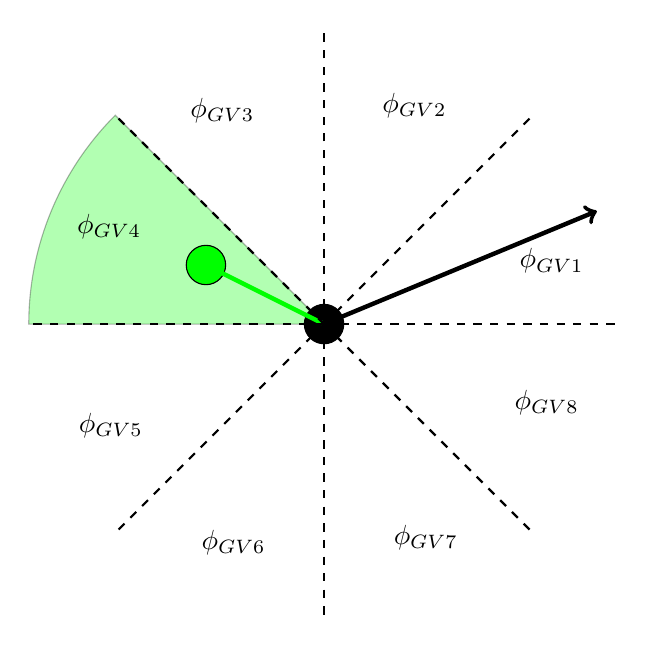
\begin{tikzpicture}[scale=2.5]
	
	\fill [fill=green, opacity=0.0] (0.0,0.0) circle [radius=1.5];
	\draw [fill=green, opacity=0.3] 
	(0,0) -- (-1.5,0) arc(180:135:1.5) -- cycle;
	
	\draw [fill=black] (0,0) circle [radius=0.1];
	\draw [->, ultra thick] (0,0) -- (22.5:1.5);
	
	\draw [fill=green] (-0.6,0.3) circle [radius=0.1];
	\draw [->, ultra thick, green] (0,0) -- (-0.6,0.3);
	
	\draw [dashed, thick] (0,0) -- (0:1.5);
	\draw [dashed, thick] (0,0) -- (45:1.5);
	\draw [dashed, thick] (0,0) -- (90:1.5);
	\draw [dashed, thick] (0,0) -- (135:1.5);
	\draw [dashed, thick] (0,0) -- (180:1.5);
	\draw [dashed, thick] (0,0) -- (225:1.5);
	\draw [dashed, thick] (0,0) -- (270:1.5);
	\draw [dashed, thick] (0,0) -- (315:1.5);
	
	
	
	
	\node at (15.5:1.2) {$\phi_{GV1}$};
	\node at (67.5:1.2) {$\phi_{GV2}$};
	\node at (115.5:1.2) {$\phi_{GV3}$};
	\node at (155.5:1.2) {$\phi_{GV4}$};
	\node at (205.5:1.2) {$\phi_{GV5}$};
	\node at (247.5:1.2) {$\phi_{GV6}$};
	\node at (295.5:1.2) {$\phi_{GV7}$};
	\node at (340.5:1.2) {$\phi_{GV8}$};
	
	\end{tikzpicture}
	
	\caption{Goal vector bin representation. The black disk at the center of the diagram and the black arrow represents the agent's position and heading respectively. The green disk depicts the goal position, and since it lies in $\phi_{GV4}$ that bin is currently active. Note that the features are relative to the agent's orientation and thus rotate with the agent.}
	\label{fig:goal-vector-diagram}
\end{figure}

\subsubsection*{Change in orientation}
Represented by a $5 \times 1$ indicator variable, the change in orientation captures the magnitude of the change in the orientation of the agent in consecutive steps. The value ranges between $0 \degree$ -  $ 180 \degree$. This value is allocated to one of 5 asymmetric bins. The rationale behind the uneven distribution is that we have observed empirically that human motion is smooth. The bins are thus constructed in a way to put greater emphasis on smaller changes in orientation. This helps capture the nuances in human motion in greater detail leading to better encapsulation of the essence of the navigational pattern. The division of the range is shown in \autoref{tab:orientation-change-bins}.

\begin{table}[!htbp]

    \begin{center}
        \renewcommand{\arraystretch}{1.3}
        \begin{tabular}{|c|c|}
            \hline
            \textbf{Feature} & \textbf{Threshold} \\
            \hline
            $\phi_{O1}$ & $\alpha_{OC} \in \left[ 0 , \frac{\pi}{9} \right)$ \\
            
            $\phi_{O2}$ & $\alpha_{OC} \in \left[ \frac{\pi}{9} , \frac{2\pi}{9} \right)$ \\
            
            $\phi_{O3}$ & $\alpha_{OC} \in \left[ \frac{2\pi}{9} , \frac{3\pi}{9} \right)$ \\
    
            
            $\phi_{O5}$ & $\alpha_{OC} \in \left[ \frac{3\pi}{9} , \frac{4\pi}{9} \right)$ \\
            
            $\phi_{O6}$ & $\alpha_{OC} \in \left[ \frac{4\pi}{9} , \pi \right)$ \\
            \hline
        \end{tabular}
        \caption{Bin thresholds orientation change features.}
    \label{tab:orientation-change-bins}
    \end{center}
\end{table}
\subsubsection*{Deviation from the goal}
The deviation from goal captures the magnitude of the angle between the vector to the goal from the current position of the agent and the current orientation vector of the agent. The value ranges from $0 \degree$ - $ 180 \degree$ which is again asymmetrically divided into 4 bins ($4 \times 1$ indicator variable), with greater emphasis on the smaller angles as described earlier (\autoref{tab:deviation-from-goal-bins}). 

\begin{table}[!htbp]
    \begin{center}
        \renewcommand{\arraystretch}{1.3}
        \begin{tabular}{|c|c|}
            \hline
            \textbf{Feature} & \textbf{Threshold} \\
            \hline
            $\phi_{GA1}$ & $\alpha_{GA} \in \left[ 0 , \frac{\pi}{8} \right)$ \\
            
            $\phi_{GA2}$ & $\alpha_{GA} \in \left[ \frac{\pi}{8} , \frac{\pi}{4} \right)$ \\
            
            $\phi_{GA3}$ & $\alpha_{GA} \in \left[ \frac{\pi}{4} , \frac{3\pi}{4} \right)$ \\
            
            $\phi_{GA4}$ & $\alpha_{GA} \in \left[ \frac{3\pi}{4} , \pi \right]$ \\
            \hline
        \end{tabular}
        \caption{Bin thresholds for deviation from the goal.}
          \label{tab:deviation-from-goal-bins}
    \end{center}
\end{table}

\subsubsection*{Speed}
The current speed of the agent is quantized and represented in the form of a $6 \times 1$ indicator variable. 
%\begin{table}[htbp]
%    \caption{Thresholds for the qantization of the speed of the agent.}
%    \label{tab:speed-quantization}
%    \begin{center}
%        \renewcommand{\arraystretch}{1.3}
%        \begin{tabular}{|c|c|}
%            \hline
%            Raw speed & Speed bin \\
%            \hline
%            0 - 0.2 & 0 \\
%            0.2 - 0.4 & 1 \\
%            0.4 - 0.6 & 2 \\
%            \hline
%        \end{tabular}
%    \end{center}
%    \end{table}

\subsection*{The local information}
Taking inspiration from previous work in this field \cite{fahad_learning_2018} \cite{vasquez_inverse_2014}, we use spatial bins to effectively divide the region surrounding the agent into discrete segments and calculate a `risk' metric for each of these bins.
    \begin{figure}[htbp]
	\centering
	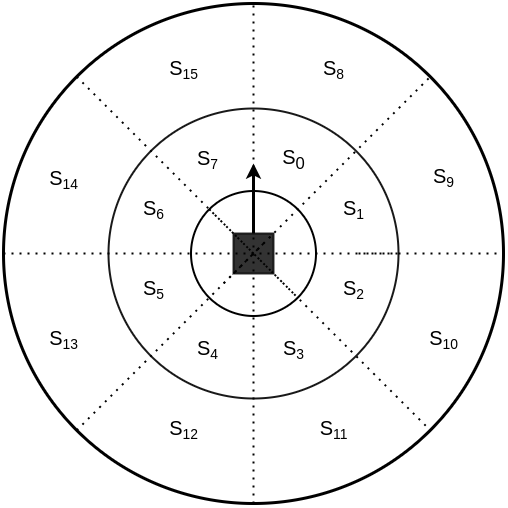
\includegraphics[width=0.5\linewidth]{figures/risk_features_spatial_bins.png}
	\caption{Segmentation of the local area around the agent. The black square and the arrow denotes the agent and its current direction of heading respectively.}
	\label{fig:risk_local_bins}
\end{figure}
\subsubsection*{Creation of the bins}
There are $16$ spatial bins surrounding the agent arranged in two concentric circles. $8$ equal divisions of the region between the agent and the inner circle form bin $1-8$. Similarly, the divisions in the region between the first and the second concentric circle form bins $9 - 16$.
\subsubsection*{Calculation of the risk}
Oxford English Dictionary defines `risk' as ``the possibility of loss, injury, or other adverse or unwelcome circumstance; a chance or situation involving such a possibility'' \cite{oxford_dictionary}. In this context, `risk' can be loosely correlated to the likelihood of a collision with a nearby obstacle/pedestrian. As a property of the spatial bins, it implies the possibility of a collision with an obstacle located in the given bin. 
The risk is divided into 3 levels: high, low, and medium.
\begin{itemize}
    \item High risk:
When the relative motion of an obstacle is towards the agent and can lead to a collision if not intervened.
    \item Low risk:
When the relative motion of an obstacle is away from the agent.
    \item Medium risk:
Anything in between.
\end{itemize}
The calculation of the risk values are based on the following entities:
\begin{align}
    \vec{o}_{rel} = & \;\; \vec{o}_{obs} - \vec{o}_{agent}  \\
    \vec{d}_{rel} =  &\;\; \vec{d}_{agent} - \vec{d}_{obs} \\
    \theta_{risk} =  & \;\; \angle (\vec{o}_{rel}, \vec{o}_{rel}) \\
    \mathbf{s}_{obs} = & \;\; \tan(\theta_{risk}) \times |\vec{d_{rel}}| \\
    \mathbf{T} = & \;\; \text{agent witdh} + \text{obstacle witdh}
\end{align}
where $\vec{o}_{rel}$ is the relative orientation of the obstacle w.r.t the agent, $\vec{d}_{rel}$ is the relative position of the agent w.r.t to the obstacle, $\theta_{risk}$ is the angle between the vectors, $\vec{o}_{rel}$ and $\vec{d}_{rel}$,  $\mathbf{s}_{obs}$ is the estimated safety margin between the agent and the obstacle and $\mathbf{T}$ is a predefined value which if maintained between the agent and an obstacle should guarantee a collision-free trajectory.\\
An obstacle is marked as `high risk' when $\theta$ is less than $90\degree$ and the safety margin is less than $\mathbf{T}$. The rationale behind this is,  $\theta$ < $90 \degree$ indicates that the involved objects are moving towards each other. Additionally, if the objects are close by, i.e. $ < \mathbf{T}$, then this describes a condition where two objects in close proximity are moving towards each other: a circumstance that is likely to encounter a collision.  If $\theta$ > $90 \degree$, this indicates that the obstacle is moving away from the agent and hence chances of collision are less and hence low risk. Anything that does not fall in the above two categories are considered as medium risk. The risk calculation conditions and values are summarized in \autoref{risk-categorization-table}
%\thcomment{I do not have any citation or study to back the classification but I have added a justification based on common sense if that helps.}
\begin{table}[htbp]
    \begin{center}
        \renewcommand{\arraystretch}{1.3}
        \begin{tabular}{|c|c|}
            \hline
            \textbf{Risk value}& \textbf{Risk condition} \\
            \hline
            High & $\theta < 90\degree$ \&  $\mathbf{s}_{obs}$ < $\mathbf{T}$   \\
            
            Low & $\theta > 90\degree$\\
            
            Medium & otherwise \\
            \hline
        \end{tabular}
    	 \caption{Categorization of the risk.}
		\label{risk-categorization-table}
    \end{center}

\end{table}
\par
The risk value of each bin is represented using a $3 \times 1$ indicator variable. The risk is calculated for individual obstacles present in a bin separately. In the event of a spatial bin containing more than one obstacle with varying degrees of risk, the risk value assigned to that bin is the highest obtained among all the obstacles that fall under that spatial bin.
\begin{figure}[!htbp]
	\centering
	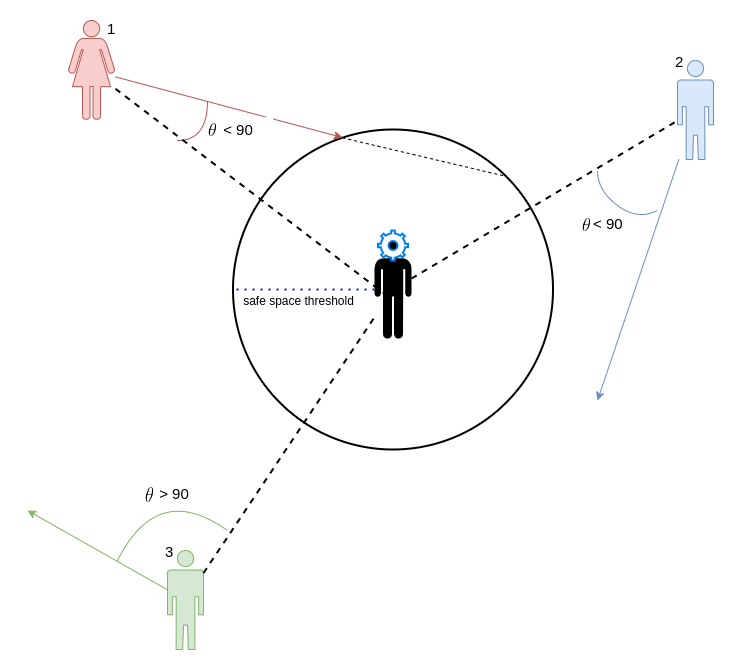
\includegraphics[width=\linewidth]{figures/risk_picture.png}
    \label{fig:risk-calculation}
    \caption{A pictorial representation of how the risk is classified. Pedestrian $1$, $2$ and $3$ falls under the category of `high' risk, `medium' and `low' risk respectively.}
\end{figure}


%\begin{figure}
%	\label{fig:agent-perspective-risk-features}
%	\begin{subfigure}[t]{.5\linewidth}
%
%		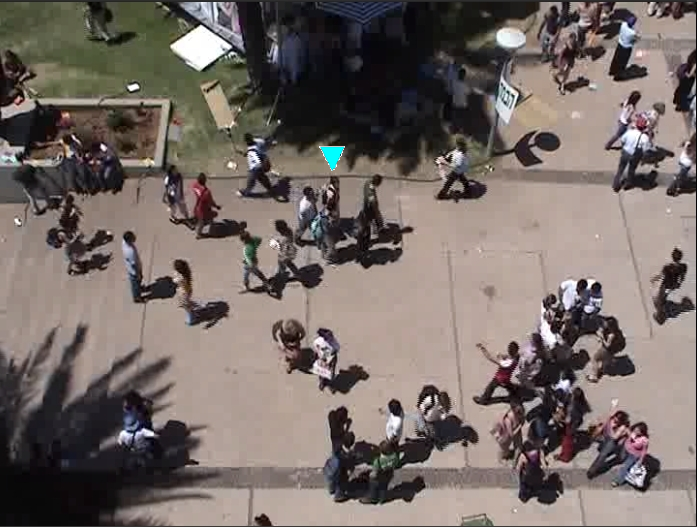
\includegraphics[width=.95\textwidth]{figures/screenshot_video_frame_agent_perspective.png}
%		\label{fig:agent-perspective_screenshot}
%		\caption{A frame from the UCY dataset. The pedestrian which is the acting agent for the current episode is marked with a blue triangle.}
%	\end{subfigure}
%	\begin{subfigure}[t]{.5\linewidth}
%		\centering
%		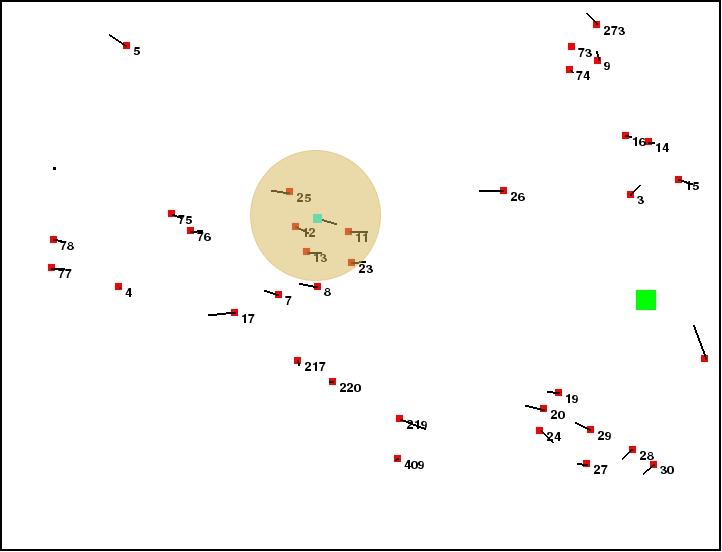
\includegraphics[width=.95\textwidth]{figures/env_screenshot_agent_perspective.png}
%		\label{fig:agent-perspective_env}
%		\centering
%		\caption{Representation of the video frame in the in-house built environment. The blue square represents the acting agent, the red squares represent other pedestrians (obstacles), and the green square represents the goal. The yellow circle around the agent is the area around the agent taken into consideration while computing the local information used by the agent.} 
%	\end{subfigure}
%	\begin{subfigure}[b]{\linewidth}
%		\centering
%		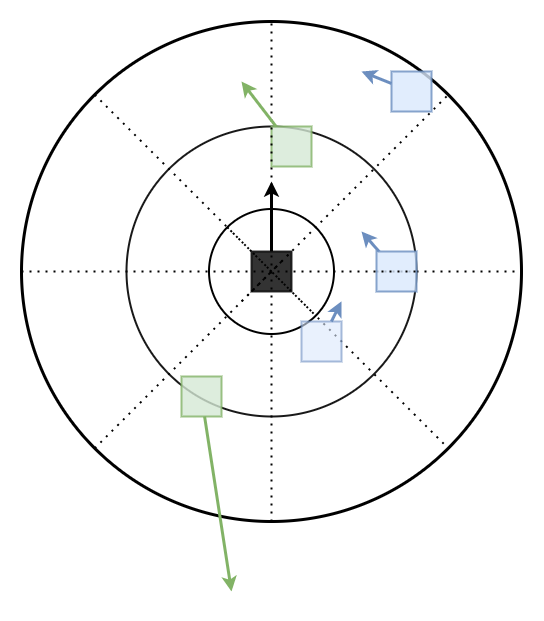
\includegraphics[width=.4\textwidth]{figures/agent_perspective_recreated.png}
%		\label{fig:agent-perspective_agent-perspective}
%		\caption{The local information from the frame as perceived by the agent using the risk features. The spatial bins are represented by the concentric circles around the agent (black square) and the dotted lines. The squares in green mark pedestrians which pose low risk, while the ones in blue denote medium risk.}
%	\end{subfigure}
%\end{figure}


\begin{figure}[!htbp]
	\label{fig:agent-perspective-risk-features}
		\centering
		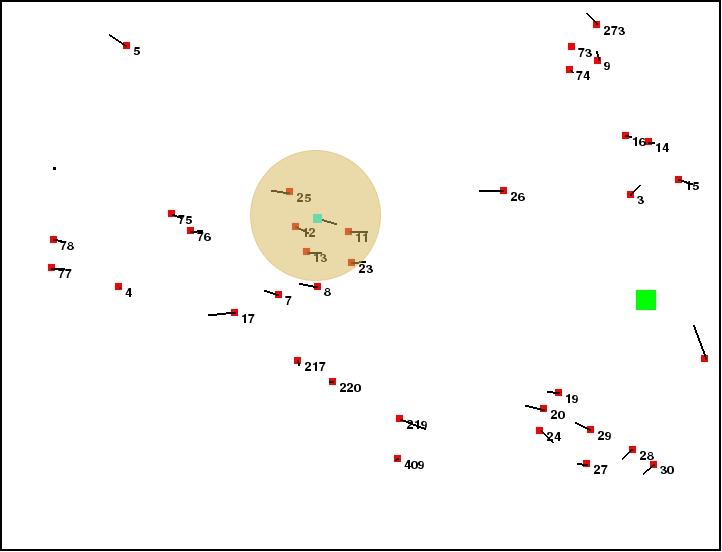
\includegraphics[width=\textwidth]{figures/env_screenshot_agent_perspective.png}
		\label{fig:agent-perspective_env}
		\centering
		\caption{A screenshot of a frame populated with human obstacles.} 
\end{figure}

\begin{figure}[!htbp]
		\centering
		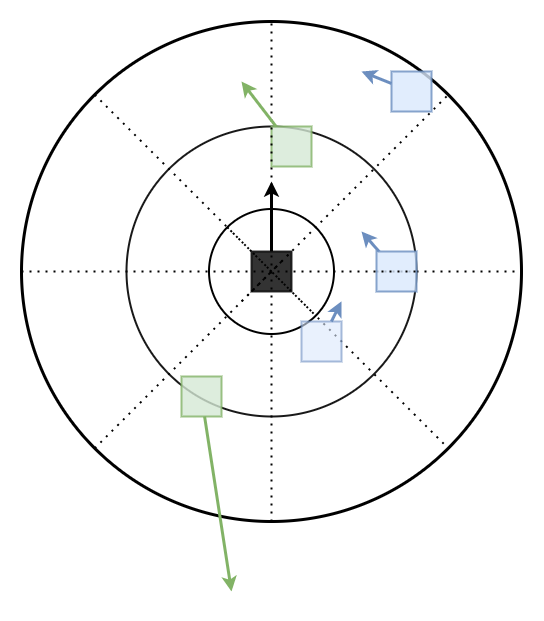
\includegraphics[width=\textwidth]{figures/agent_perspective_recreated.png}
		\label{fig:agent-perspective_agent-perspective}
		\caption{The local perspective of the agent in the frame. The arrows mark the relative velocity of the nearby pedestrians w.r.t. the agent. Risk classification is color-coded as mentioned earlier.}
\end{figure}




%Additionally, we also introduce a \textbf{smoothing technique} for the calculated svf. \\
%\textbf{What is smoothing?}\\
%In the traditional way of calculating the SVF, the observation of a given state contributes to the increment of the visitation frequency of that state by 1. 
%Instead for a single observation, we opt for the increment in the visitation frequency of a set of neighboring states based on the closeness of the neighboring states to the state observed. Here smoothing is defined as the distribution of the visitation weight of a state over its set of neighboring states based on their spatial similarity.\\
%\textbf{Why smoothing?}
%Having a 1 to 1 mapping between the observation and the increment of the SVF misses out on the fact that not all states \textit{are equally different.} \textbf{differ from each other in equal magnitude} \\
%\textbf{For example:} consider 3 different states, which differ only in their goal location component. Now, if two of the states indicated the goal to be in the $2^{nd}$ spatial bin and $3^{rd}$ spatial bin, then the difference between these two states is smaller than a $3^{rd}$ state where the goal is in the $6^{th}$ bin.
%This inequality in the differences among different states is accounted for in the smoothing, by increasing the weighted increment of a set of neighboring states of the observed state (based on their similarity) rather than increasing the value of the observed state only. \\ 
%\textbf{How smoothing?}
%The state vector comprises of different components, and the 'smoothed' state is obtained by convolving a smoothing kernel to each of them separately. The values used in the kernel, and the type of convolution applied depends on the nature of the spatial division the feature represents and is summarised in the Table \ref{conv-table}.
%
%\begin{table}
%    \caption{Table showing the details of the convolution used for smoothing the state feature vector.}
%    \label{conv-table}
%    \begin{center}
%        \renewcommand{\arraystretch}{1.3}
%        \begin{tabular}{|c|c|c|}
%            \hline
%            Feature component & Convolution Kernel & Convolution type\\
%            \hline
%            Relative goal orientation & $ [0.1, \;0.8, \; 0.1 ]$ & Wrap  \\
%            
%            Change in orientation & $[ 0.1, \; 0.8; \;0.1 ]$ & Same \\
%            
%            Deviation from goal & $[0.9,\; 0.1]$, $[0.1,\; 0.9]$,
%                                          $[0.05, \; 0.9, \; 0.05]$, $[0.1,\; 0.9]$ & Same \\
%            Local spatial bins & $[ 0.1, \; 0.8,\;0.1 ]$ & Wrap \\
%            Speed info & $[ 0.1, \; 0.8,\;0.1 ]$  & Same \\
%            \hline
%        \end{tabular}
%    \end{center}
%\end{table}


\chapter{The environment}
\label{ch:chapter5}
\label{ch:enviornment}
%\thcomment{I have made some major changes here. I have not removed any parts but I have removed all of the implementation details. However, I have kept some of the mathematics governing the calculation of the speed and orientation. }
This chapter presents a detailed description of the environment used for conducting the experiments. The environment, implemented using Pygame \cite{pygame}, portrays the world as a rectangular area viewed from a top-down perspective (bird's eye view). 
The size of the world can be set by altering the rows and columns during initialization. These values denote the size of the world in pixels.

The environment follows the image coordinate system: with the center at the top left corner and each position on the map is indicated by a 2-dimensional vector containing the row and column value respectively.\\
\section{Components}
3 key components populate the environment: 
\begin{itemize}
    \item The agent.
    \item The goal.
    \item The obstacles.
\end{itemize}
\subsection{The agent}
The agent represents the entity being controlled by an external controller. At any given moment, the state of the agent has three properties: position, speed, and orientation.
\begin{enumerate}
    \item Position: The current coordinates of the agent (in pixel coordinates) on the map.
    \item Speed: The current speed of the agent.
    \item Orientation: A unit vector along the velocity vector of the agent.
\end{enumerate}
To navigate the environment, the agent controls two aspects of its motion: its speed and orientation.
Unlike most stock environments, this supports both continuous and discrete action space. These are elaborated in \autoref{subsec:action-space}.
\subsection{The goal}
The goal is a pre-designated area of the map where on arrival marks the end of an episode with a success. It is represented by a green rectangle. Like the agent, the size of the goal area can be customized as per the requirement of the experiment. For now, the environment just has provision for static goals. That being said, the environment does come with the provision to randomly alter the position of the goal at the end of each episode.


\subsection{The obstacles}
There are 3 ways of putting obstacles in the map each of them serving a different purpose.
\begin{enumerate}
\item \textbf{Individual specification}: This is aimed at quick deployment of  a small number of static obstacles in different locations of the map and is best suited for use in the sanity check of a controller.
\item \textbf{Obstacle map}: It is the primary method of initializing static obstacles on the environment. The dimensions of the image dictate the size of the environment. The resolution of the obstacle map recreated in the environment can be adjusted as per requirement. A higher resolution portrays a obstacle map faithful to the original image, retaining finer details. The trade off to this is the large number of obstacles used to create the obstacle map which increases exponentially with the increase in resolution.
%\item \textbf{Using a list:}
%The information for the placement of the obstacles can be passed in the form of a list, where each element in the list is a Numpy array containing the pixel coordinate ([row, col]) of the obstacle. This is primarily useful when the number of obstacles to be deployed is small. Although it severely limits the number and the configuration of the obstacles that can be placed in the map, it is ideal for performing a quick initialization or a brief sanity test of a controller in a short time without investing in creating an obstacle map or an annotation file.
%\item \textbf{Using an obstacle map:}
%This is the primary way of initializing the environment with static obstacles. In this case, the path to an image file is provided during initialization. This image is then read by the environment to obtain the size of the map and the obstacle configuration. 
%The dimensions of the image determine the size of the map. Comprehending the obstacle configuration is also straight forward. Any red pixel, pixel falling in the color range of ($150$, $0$, $0$) to ($255$, $0$, $0$) is categorized as an obstacle. While defining each pixel as an individual obstacle renders the most accurate recreation of the obstacle configuration from a given image, it is inefficient as it generates an unnecessarily large number of obstacles on the map.
%This is redundant as for most of the cases, instead of having pixel-sized obstacles,  these obstacles can be grouped into bigger cells often without loosing too much information or diverging too much from the original configuration. The grouping can be adjusted by tuning the obstacle-width parameter in the environment.  Setting the width to one sets the size of an individual obstacle to $1$. This retains the highest amount of information (basically pixel-by-pixel information) from the obstacle map. Increasing the width groups pixels in the image to form obstacles of the given width, which drastically reduces the number of obstacles at the cost of introducing a pixelation effect in the final obstacle map.
%\textbf{A set of 3 images: obstacle image, and its comparison with changing obstacle size}

\begin{figure}[!h]
	\begin{subfigure}[t]{.5\textwidth}
		\centering
		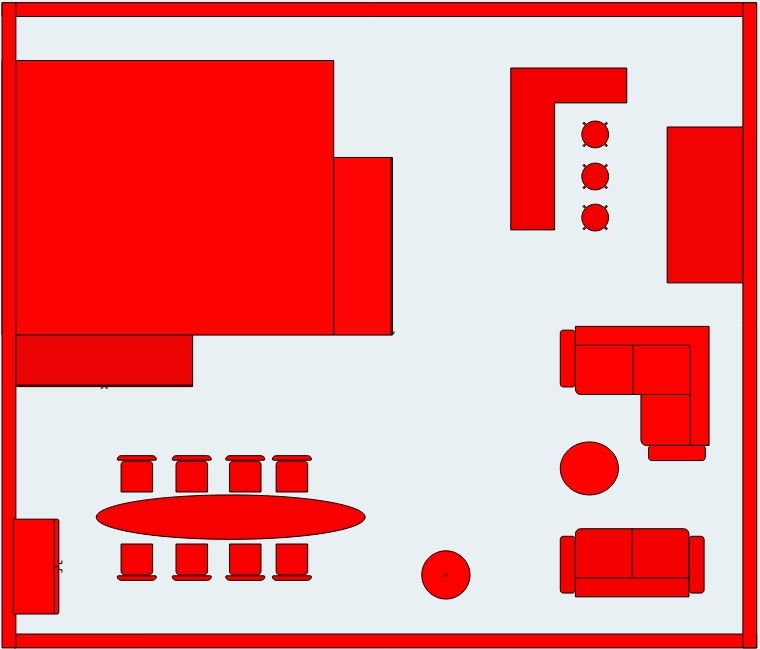
\includegraphics[width=.95\linewidth]{figures/real_map.jpg}
		\caption{The original obstacle map}
		\label{fig:obsmap_sfig1}
	\end{subfigure}%
	\begin{subfigure}[t]{.5\textwidth}
		\centering
		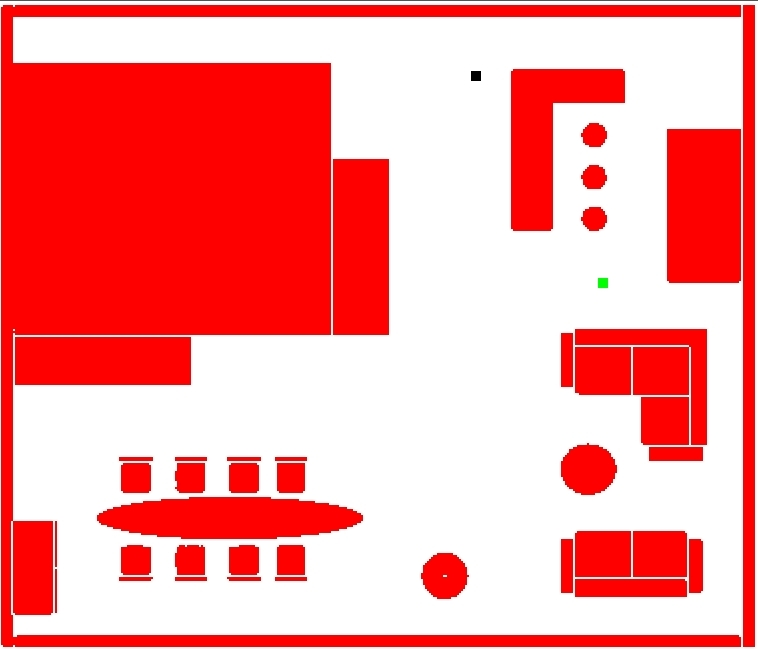
\includegraphics[width=.95\linewidth]{figures/obs_width_2_total_obs_51348.jpg}
		\caption{Obstacle width: 2, number of obstacles: 51348}
		\label{fig:obsmap_sfig2}
	\end{subfigure}%
\end{figure}

\vfill
\begin{figure}[!h]\ContinuedFloat
	\begin{subfigure}[b]{.5\textwidth}
		\centering
		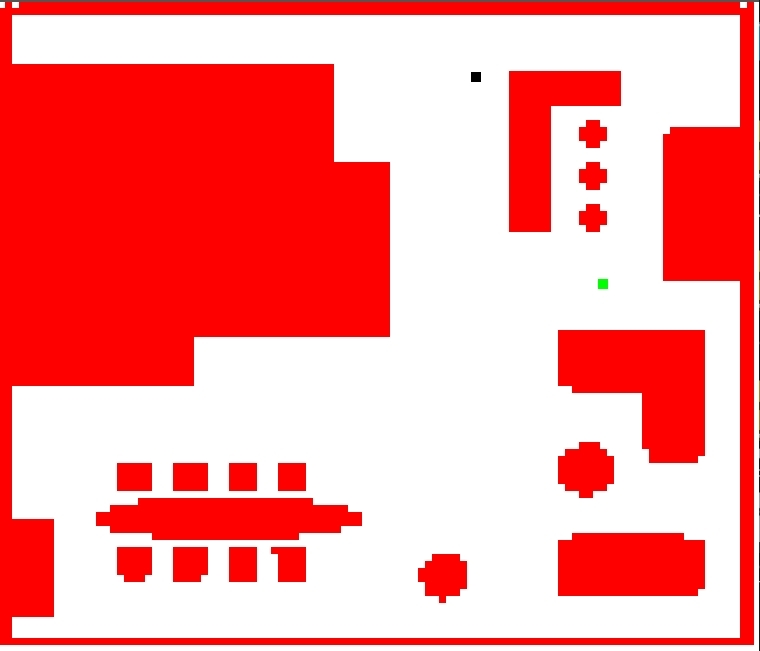
\includegraphics[width=.95\linewidth]{figures/obs_width_7_total_obs_4293.jpg}
		\caption{Obstacle width: 7, number of obstacles: 4293}
		\label{fig:obsmap_sfig3}
	\end{subfigure}
	\begin{subfigure}[b]{.5\textwidth}
		\centering
		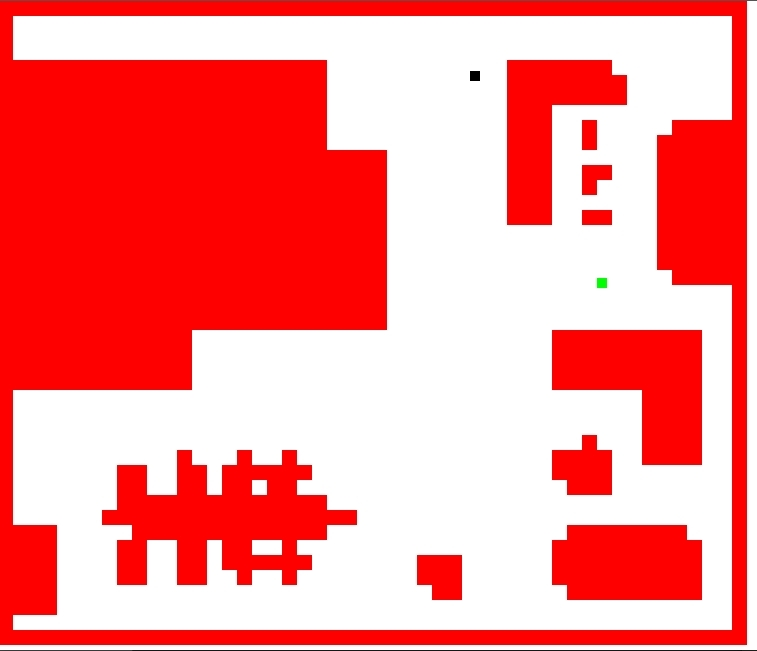
\includegraphics[width=.95\linewidth]{figures/obs_width_15_total_obs_996.jpg}
		\caption{Obstacle width: 15, number of obstacles: 996}
		\label{fig:obsmap_sfig4}
\end{subfigure}
	\caption{Recreation of the given image in the form of an obstacle map in the environment at different resolutions.}
	\label{fig:fig}
\end{figure}


\item \textbf{Annotation file}: It is used to populate the environment with dynamic obstacles. The annotation files contain frame-by-frame details of the position of all the entities of the environment at any given time step. 

\begin{figure}[htbp]

		\centering
		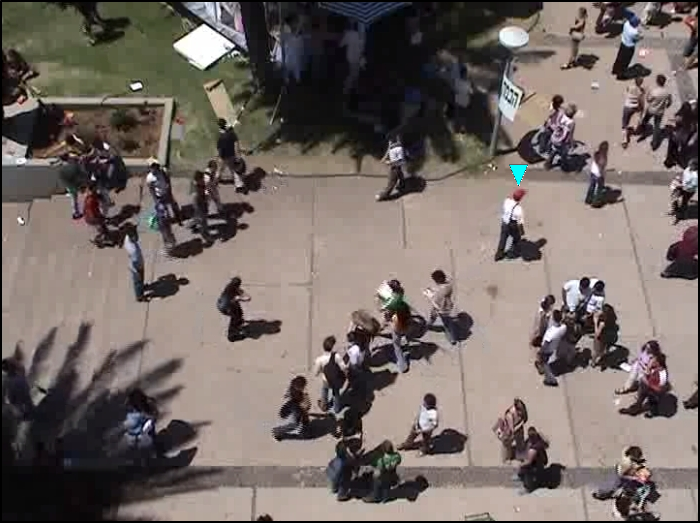
\includegraphics[width=.95\linewidth]{figures/video_frame_students_with_agent_pointer.png}
		\caption{Frame from the original video}
		\label{fig:anno_sfig1}
\end{figure}
\vfill
\begin{figure}[htbp]
		\centering
		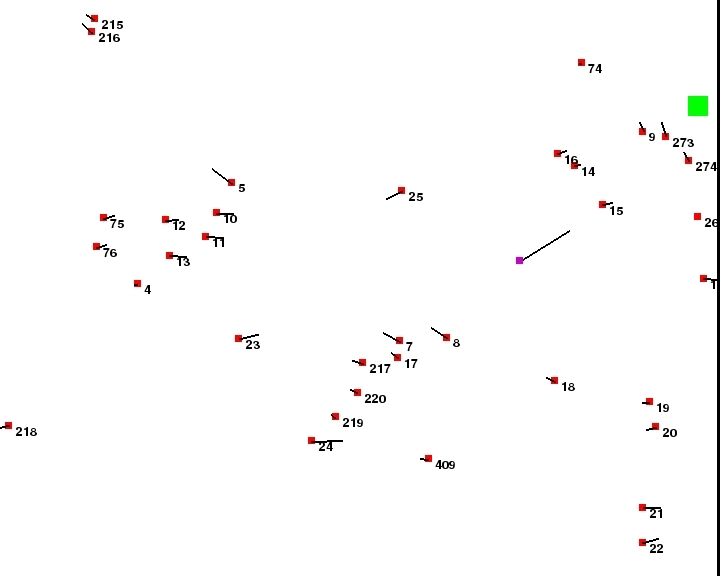
\includegraphics[width=0.9\linewidth]{figures/env_screenshot.jpg}
		\caption{Corresponding frame recreated in the environment using the annotation file.}
		\label{fig:anno_sfig2}

\end{figure}
\end{enumerate}


\section{Input spaces and observation} 
\label{subsec:action-space}
The environment has provisions for both discrete and continuous action space.
\begin{enumerate}
    \item \textbf{Continuous action space}: In this mode, the agent receives two separate inputs controlling its change in speed and orientation. This, along with the current state of the agent is used to compute the position, velocity, and orientation of the agent for the next state as shown in \autoref{eq:next_state_agent} and \autoref{eq:next_state_agent2}.\\
%   \begin{align}
%	\nabla_{orient} & = \texttt{action}_{0}\\
%	\nabla_{speed} & = \texttt{action}_{1}
%	\end{align}
%    where $S_{max}$ is the maximum speed of the agent and $\nabla_{orient}$ and $\nabla_{speed}$ are the change in orientation and speed at a given step respectively.
    
    \item \textbf{Discrete action space}: This mode makes a single choice over a set of predefined actions that control the speed and orientation of the agent. In the current version, the rate of change in speed and orientation is divided into $7$ and $5$ bins respectively thus allowing the agent to take one out of the $35$ predefined actions made from the combination of the two factors. The underlying control is similar to that of the continuous mode.\\
%    \begin{align}
%	    \nabla_{orient} & = \texttt{Arr}_{orient}[\texttt{act}_{t}\%7]\\
%	    \nabla_{speed} & = \texttt{Arr}_{speed}[\texttt{act}_{t}/7]   
%    \end{align}
%    where $\texttt{act}_{t} \in \mathbb{Z} [ 0, 35]$, $\texttt{Arr}_{orient}$ is the orientation array and, $\texttt{Arr}_{speed}$ is the speed array.\\
    The speed and orientation of the agent is updated at every time step using \autoref{eq:next_state_agent}
    \begin{align}
		\label{eq:next_state_agent}
		%\texttt{speed}_{t+1} & =\texttt{min\{} \texttt{max\{(}\texttt{speed}_{t} + \texttt{action}[0]\texttt{), 0\}, } S_{max}\}\\
		v_{t+1} & = \{ {v}_{t} + \delta_{v} :  0 \le v_{t+1} \le S_{max} \}\\
		\label{eq:next_state_agent2}
		%\texttt{orient}_{t+1} & = (\texttt{orient}_{t} + \texttt{action}[1]) \% 360
		o_{t+1} & = \{ {o}_{t} + \delta_{o} :  0^{\circ} \le v_{t+1} \le 360^{\circ}\}
	\end{align}
	where, $v_{i}$ and $o_{i}$ are the speed and orientation of the agent at time step $i$, $\delta_v$ and $\delta_{o}$ are the change in speed and orientation the agent is subjected to at a given time step, and, $S_{max}$ is the maximum permitted speed of the agent. The speed of the agent is measured in pixels per frame.\\ 
	The permitted range of the rate of change in speed and orientation are summarized in \autoref{tab:env_kinematic_ranges}.
\begin{table}[tbhp]
	\begin{center}
	  \renewcommand{\arraystretch}{1.3}
		\begin{tabular}{|c|c|c|}
			\hline
			\textbf{Motion component} & \textbf{Lower bound} & \textbf{Upper bound}\\
			\hline
			Change in speed per time step & $-0.4$ &  $+0.4$ \\
			Change in orientation per time step & $30^{\circ}$ anti-clockwise & $30^{\circ}$ clockwise\\
			Speed & 0 & 2\\
			Orientation & $0^\circ$ & $360^{\circ}$\\
			\hline
		\end{tabular}
	\end{center}
	\caption{Valid ranges of different motion components of the environment.}
	\label{tab:env_kinematic_ranges}
\end{table}
\end{enumerate}

\subsubsection{The Observation:}
The observation from the environment returns a tuple of 4 elements: ( $S$, $\rho$, $\mathbf{d}$, $\iota$ ), where
$S$ is the state of environment containing the information relating to the agent, goal, and the obstacles for a given time step,
$\rho$ is the reward obtained at a given time step, $\mathbf{d}$ is a Boolean flag that indicates the completion of the current episode, and $\iota$ contains any extra information the environment might want to convey.
\section{Additional features}
Additionally, the environment comes with a set of options that provide added flexibility and customization while training and evaluating IRL agents.
\subsubsection{Training modes:}
The environment supports 3 types of training modes:. 
\begin{enumerate}
    \item \textbf{Fixed respawn:} The starting and goal position of the agent remains the same throughout the training process.
    \item \textbf{Random respawn:} For every episode, the agent and the goal spawns at random locations on the map. 
    \item \textbf{Replace a pedestrian:} For every episode, the agent assumes the role of a randomly selected pedestrian. Once a pedestrian is selected, the pedestrian is ignored as an obstacle for that episode. The initial position of the agent is set to the coordinated of the pedestrian in its first frame of appearance. Similarly, the goal is set to the coordinates of the pedestrian in the final frame.
    This mode is especially useful for training IRL models because demonstrations from experts for navigation are the optimal demonstrations for a particular configuration of goal and obstacle. Placing the agent in the exact context enables the agent to observe the same state distribution as the expert, which helps to maintain the relevance of the expert demonstrations. 
\end{enumerate}
Features available for testing of the environment:
The environment was designed primarily for the development of IRL methods for navigation, and also comes with built-in tools to test IRL methods.
\subsubsection{Deployment of ghost}
IRL agents learn from demonstrations. Creating meaningful metrics to evaluate their performance is elusive, which is why we resort to using IRL in the first place. One simple and effective way of conducting a performance analysis would be to subject the agent to the same conditions as the expert and compare and contrast their behaviors. This is exactly what the environment facilitates. We define the `ghost' of a given pedestrian as an entity that traces the exact path, both spatially and temporally, as the pedestrian without interacting or interfering with any other entities of the environment. This greatly benefits in the comparison of the performance of the agent to the expert.

\subsubsection{User control}
The environment also has a provision to let an external user control and agent and navigate the crowds. There might be cases where there are not enough expert demonstrations available to perform proper training. In that case, the size of the expert demonstration set can be bolstered by letting humans take control of the agent and generate additional expert demonstrations.

%The agent can be controlled by a mouse pointer and action is registered only at the time of the click of the left mouse button. Once a click is registered on the map, the direction and magnitude of the vector joining the current position and the location of the click are taken as the desired orientation and speed respectively.  
%The orientation action is then calculated based on the difference between the current orientation of the agent and comparing that with the desired direction. If there is a difference between the two, and a change in the current heading direction of the agent is warranted, then the action to inflict the change is then decided based on the magnitude and sign of the change needed relative to the current heading direction of the agent to minimize the difference.
%The speed action is also calculated in a similar manner, where the magnitude of the difference vector is treated as the desired speed, and based on the current speed of the agent action is taken to minimize the difference.

\subsubsection{Custom scene generation}
The environment has provisions to create custom dynamic scenarios, where the motion of each of the pedestrians can be predefined. This is a very handy tool for creating and testing the agents in situations that are hard to come across or simply unavailable in the available data sets.\\





\chapter{Experiments and results}
\label{ch:chapter6}
\label{ch:6}
\subsubsection*{Overview}
In this chapter, we report the results from various subjective and objective experiments conducted to show a comprehensive performance comparison of our method to that in the existing literature. All the experiments are conducted in the simulator described in \autoref{ch:enviornment}. \\
We perform baseline comparisons in \autoref{sec:baseline-evaluation}: comparing our IRL method to a model-based potential field controller, and a data-driven RL agent trained in a similar setting using a simple yet dense hand-crafted reward function. This helps in demonstrating the difference in the performance of agents coming from different training methods and how our IRL pipeline fare against them.\\
 Feature representations play a vital role in an IRL pipeline. Keeping that in mind, we dedicate \autoref{sec:comparing-other-featreps} to comparing the performance of IRL agents trained in a similar setting but different feature representations.\\
 Finally, \autoref{sec:generalization} is dedicated to testing the generalization capabilities of our method, where we repeat our experiments on out-of-distribution data.

%Getting tricky scenarios that help showcase the subtle subjective aspects of a navigating agent from the real-world video might be difficult and indeed with the time and effort spent scrolling through the videos to find these are hard, so we also generate some synthetic scenarios to check some of the specific, more advanced subjective behaviors of the IRL and how that differs to that of the RL.
%
%The last subsection looks into the reward function: the second, and unfortunately, in most of the cases, ignored part of the equation. We try to visualize and interpret the reward function in an attempt to get a better insight into the functioning of our agent.

\section{Experimental setup and training details}
\label{sec:exp-setup}
In this section we outline our experimental setup and training details. The maximum entropy deep inverse reinforcement learning (MEDIRL) pipeline is run for $100$ epochs. The reinforcement learning algorithm \cite{mnih_actor_critic_2016} running in the inner loop is run for a predefined number of episodes. An episode terminates when the agent reaches the goal, hits an obstacle, or exceeds the limit of frames assigned to an episode. Both the policy and reward networks have a relatively simple architecture. The reward network has an input layer of width equal to that of the size of the feature vector and a single hidden layer consisting of $256$ nodes. Both the layers use Exponential Linear Unit (ELU) \cite{elu} activation function. The hidden layer is followed by a output layer that returns a real value which uses a Tanh activation function. The policy network as a similar architecture: an input layer whose size is dictated by the size of the feature vector followed by a hidden layer with $256$ nodes and ELU activation. From the hidden layer, the network bifurcates to the action head and the value head, forming the actor and the critic network. The action head consists of a linear layer followed by a Softmax layer while the value head consists of only a linear layer that outputs a real number.

%with an exponential linear unit (ELU) \cite{exponential-linear-unit} as the activation function and adaptive moment estimation (Adam) \cite{adaptive-moment-estimation} as the choice of the optimizer. The learning rate for the policy and reward network is set to $0.001$ and $0.0005$ respectively.

\begin{figure}
    	\begin{subfigure}[b]{.5\textwidth}
    	\centering
    	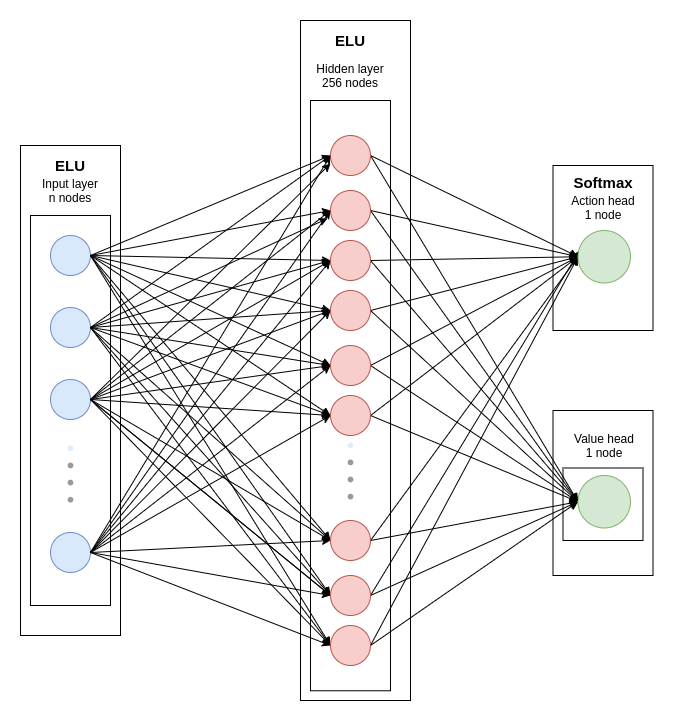
\includegraphics[width=.9\linewidth]{figures/policy_network.png}
    	\caption{The structure of the policy network.}
    	\label{fig:policy-network}
    \end{subfigure}%
    \begin{subfigure}[b]{.5\textwidth}
    	\centering
    	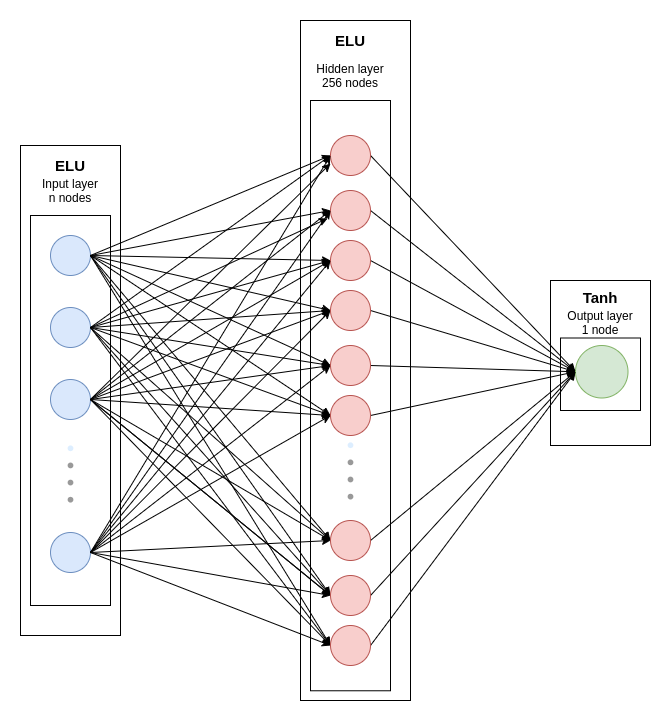
\includegraphics[width=.9\linewidth]{figures/reward_network.png}
    	\caption{The structure of the reward network.}
    	\label{fig:reward-network}
    \end{subfigure}%
\caption{A graphical representation of the networks used in the training.}
\end{figure}


To train our agent we select demonstrations from the UCY university students dataset \cite{lerner_crowds_by_example_2007}. It consists of trajectories of $430$ different pedestrians on a relatively busy area captured over $3$ minutes and $37$ seconds. The video is captured at $25$ fps resulting in a total of $5400$ frames. The length of the trajectories varies from $47.31$  to $2047$ with an average of $406$ frames per trajectory. A key aspect of this dataset is that the data is captured from a moderate to densely crowded scene of an open space on a university campus. This puts nominal restriction by static obstacles on the pedestrians and provides a dataset where the movements of the subjects are primarily dictated by social interaction.

%\begin{table}
%    \caption {Table containing useful information on the what is useful}
%    \label{university-students-stats}
%        \begin{center}
%        \renewcommand{\arraystretch}{1.3}
%        \begin{tabular}{|c|c|}
%            \hline
%            Property  & Value \\
%            \hline
%            Number of pedestrians &    \\
%            Avg trajectory length &  \\
%             & $\theta > 90\degree$\\
%            
%            Medium & otherwise \\
%            \hline
%        \end{tabular}
%    \end{center}
%\end{table} 

\subsubsection*{Description of the metrics utilized}
%What do we want to show? 
%\begin{enumerate}
%    \item Justify the use of IRL over RL or traditional methods.
%    \item Establish the superiority of the feature representation over other
%    \item Show that the smoothing affects the performance of the agent in a positive way.
%    \item Show the generalizability of the method. (Compare the performance metrics of the agent in the two different scenarios.)
%    \item Another benefit of IRL is the availability of the reward network. Visualization and comprehension of the reward network. 
%\end{enumerate}
%How do we show?
%
%To test the generalization capabilities of our method we train on the expert demonstrations from lone of the video and test it on data from different scenarios.

%\begin{itemize}
%        \item Training and testing on the same annotation file.
%        \item Training and testing on different annotation files.
%        \item Testing on custom scenarios.
%\end{itemize}
To get a comprehensive comparison of the performance of the agents, we compare them using different metrics, each capturing a unique characteristic of the navigation behavior exhibited by the agent. The metrics are described below:
\begin{itemize}
        \item \textbf{Reaching the goal:} The ability to reach a goal from a given position is one of the fundamental criteria to measure the performance of a navigating agent. It is calculated as the fraction of runs in which the agent successfully reaches its desired location.        
        
        \item \textbf{Collision counts:} This gives a better understanding of an agent in the event of a collision. While counting the number of successful trajectories gives an idea of the performance of an agent in collision-free paths, it fails to shed light on the degree of under performance in the cases where a collision does occur. It is calculated by counting the number of collisions the agent encounters in a single sampled trajectory.
        
        %\item \textbf{Distance to displacement ratio:} This metric captures the efficiency of the path an agent takes to move between two points. It is calculated as the ratio between the euclidean distance between the two points and the distance traveled by the agent to reach the second point from the first. So, for two agents moving from the same start and endpoints, given both of them are successful in reaching the goal, the agent taking a more direct path, is rated better than the other. (The results are shown in the form of histogram plots)

%        \item \textbf{Minimum distance over time graphs:} Indicates the minimum distance maintained by an agent throughout its entire trajectory. It can be thought of as a measure of how 'dangerously' or 'cautiously' an agent behaves while interacting with neighboring obstacles. (line graphs over time frame)
        \item \textbf{Trajectory smoothness:} Trajectories traced by people are smooth with rare occurrences of drastic change in the heading direction. This metric measures how much an agent changes its heading direction, thus the smoothness of its trajectory while negotiating obstacles or navigating in general.
        \item \textbf{Deviation from expert:}The main aim of the work is to obtain agents that navigate and interact with crowds like a human being, which is why computing the deviation or divergence from expert is one of the more important metrics we use to evaluate the agents. This performs a direct comparison between the trajectory taken by an agent and the trajectory followed by the pedestrian and is calculated as the mean squared error (MSE) between the points on the trajectory of the agent and the pedestrian (ground truth) at each time frame. All the deviation values reported in the thesis is in pixels. The comparison is performed over a range of trajectory segment lengths to showcase the short to medium term navigation capabilities of the agents. It is a measure of how much the trajectory traced by an agent conforms to the original trajectory of the pedestrian when subjected to similar conditions.\\
        Social navigation is an under-constrained problem. This is especially true for sparsely populated regions with more than one paths to a given destination. To better understand the deviation of the agents from the ground truth, we classify the pedestrians into 3 levels of difficulty: easy, moderate, and hard, based on the average number of pedestrians in the vicinity and perform separate deviation analysis on the pedestrians of each class. The idea is that a pedestrian from the `easier' class encounters relatively less crowd along its path, which in turn provides a wider choice of `good' trajectories, that does not necessarily conform to the ground truth.
        %\item \textbf{Traced trajectory of multiple agents for a particular pedestrian:} Primarily a visual tool to see how an agent performs in comparison to the ground truth.
        For the UCY university students, we arrange the set of all pedestrians according to the average density of obstacles (other pedestrians) encountered over the their trajectory and segregate them in three groups accordingly. The first $248$ pedestrians of the sorted list fall under the easy category, the next $133$ pedestrians fall under the moderate category and the rest are marked as hard as illustrated in \autoref{fig:ucy_ped_density_division}. The average number of pedestrians of each levels are detailed in \autoref{tab:ucy_difficulty_level_division}
        \begin{figure}
        	\centering
        	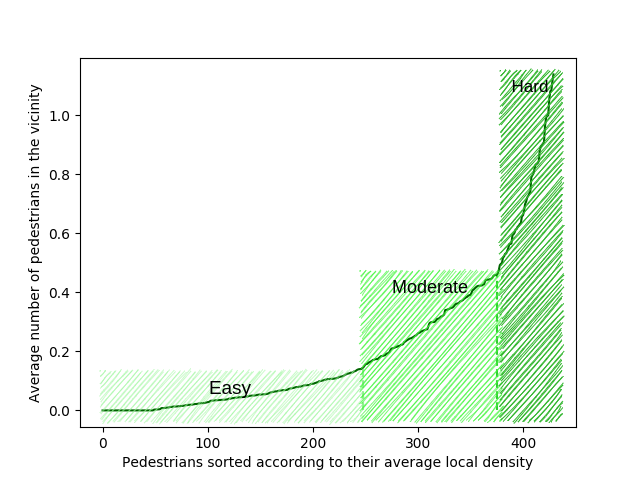
\includegraphics[width=0.8\linewidth]{plots/ucy_students_density_divisions.png}
        	\caption{Classification of the pedestrians of the UCY university students dataset according to the average density of obstacles faced over their trajectories.}
        	\label{fig:ucy_ped_density_division}
        \end{figure}
		\begin{table}[!htbp]
			\begin{center}
			\renewcommand{\arraystretch}{1.3}
				\begin{tabular}{|c|c|}
					\hline
					\multirow{2}{*}{\textbf{Difficulty level}} & \textbf{Average pedestrians} \\
										& \textbf{encountered per frame} \\
				    \hline
					Easy & $0.05$ \\
					Moderate & $0.30$ \\
					Hard & $0.73$\\
				   \hline
				\end{tabular}
			\caption{Average pedestrians encountered at each pedestrian difficulty level}
			\label{tab:ucy_difficulty_level_division}
			\end{center}
		\end{table}
\end{itemize}

\section{Baseline evaluation}
\label{sec:baseline-evaluation}
In this section we compare an agent trained using our method to two other agents: an agent trained using reinforcement learning and a potential-field controller. The RL agent is trained in the same environment as the IRL using similar training hyper-parameters and network architecture with a dense reward function shown in \autoref{tab:reward-function-summarization}.
\begin{table}[htbp]
    \begin{center}
        \renewcommand{\arraystretch}{1.3}
        \begin{tabular}{|c|c|}
        \hline
        \textbf{Condition} & \textbf{Reward assigned} \\
        \hline
        Reach goal & 1 \\
        Hit obstacle & -1 \\
        Move towards goal & $0.01 \times \text{length of the step}$ \\
        Move away from goal & $ -0.01 \times \text{length of the step}$\\
        \hline
        \end{tabular}
    \end{center}
    \caption{Reward structure used for the RL agent}
    \label{tab:reward-function-summarization}
\end{table}\\
The implementation of the potential field controller is based on \cite{khatib_1986}.\\  
\begin{figure}[htbp]
    \begin{subfigure}{0.5\textwidth}
        \centering
        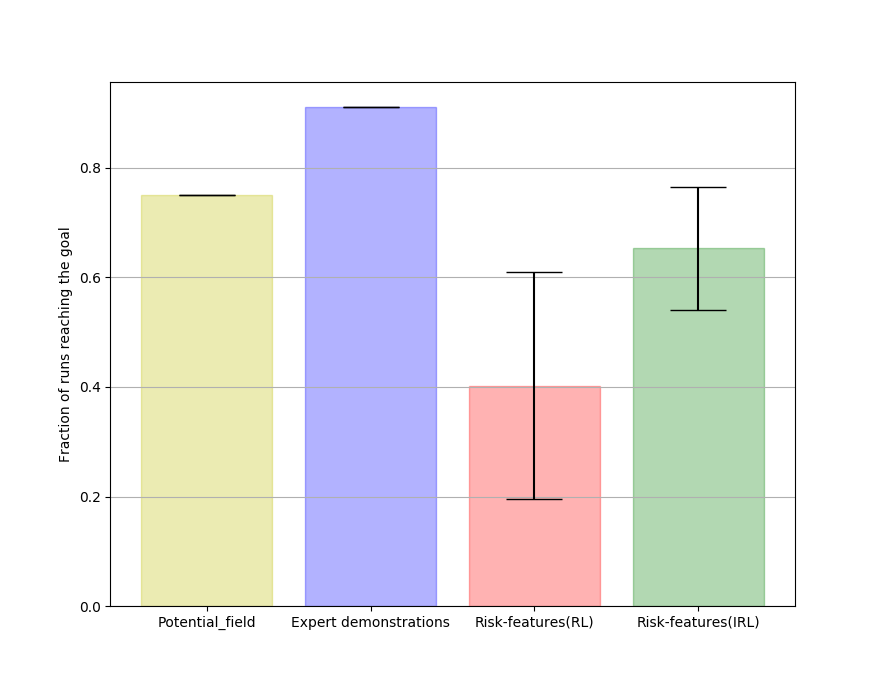
\includegraphics[width=0.95\linewidth, height=6cm]{plots/plot_without_outliers/ucy_inter_method_no_outlier/goal_reached_ucy_no_outlier_inter_method.png}
        \caption{The fraction of run successfully completed by agents trained using the different methods.}
        \label{fig:inter_method-goal_reached}
    \end{subfigure}
        \begin{subfigure}{0.5\textwidth}
            \centering
        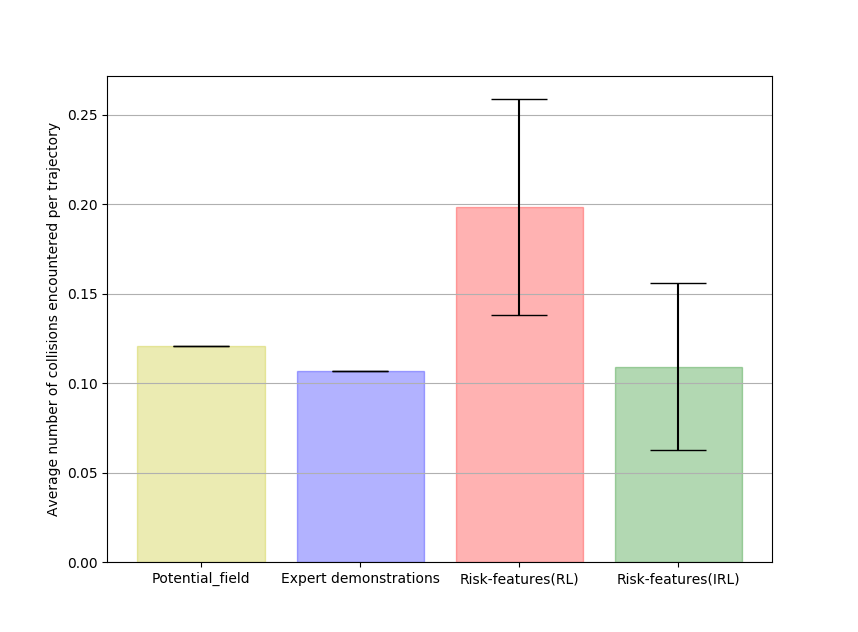
\includegraphics[width=0.95\linewidth, height=6cm]{plots/plot_without_outliers/ucy_inter_method_no_outlier/count_collisions_ucy_no_outlier_inter_method.png}
        \caption{The average number of collisions encountered by the agents in a single trajectory.}
        \label{fig:inter_method-collision_counts}
    \end{subfigure}
\caption{Comparing the fundamental properties of navigation in agents trained using different methods}
\end{figure}\\

Figure \ref{fig:inter_method-goal_reached} and \ref{fig:inter_method-collision_counts} show that out of the 3 agents, the potential field (PF) and the IRL based method are significantly better at navigating the environment with potential field slightly pulling ahead of the IRL agent in both the criteria. In the task of reaching the goal, the potential field achieves a success rate of $75.11\%$ closely followed by the IRL agent with a success rate of  $65.30\%$ and finally, the RL agent with $40.20\%$. The potential field controller enjoys about a $13\%$ greater success rate in reaching the goal, but the number of collisions encountered by the potential field controller is more, albeit by a slight margin, as compared to the IRL agent. This shows that while the IRL agent might not have the high propensity of the potential field controller to proceed towards the goal, it is does outperform the potential field controller at avoiding other pedestrians while navigating the map. This is understandable because, not often people beeline for the goal. Especially in a crowded environment, avoiding fellow pedestrians in an acceptable manner take a higher precedence. The IRL agent is trained on demonstrations from people, and so depict a similar behavior.  %This is understandable for a PF controller as they are explicitly designed to reach a goal avoiding collisions in the process, and with the absence of local-maxima, which is one of the major drawbacks of the method, the potential field agent is at its niche. 
It is also interesting to see that opting for IRL over RL as the choice of training significantly increases the objective performance of the agent.

%Figure \ref{fig:inter_method-reach_goal}, and \ref{fig:inter_method-collision_counts} shows that both, the IRL agent and the potential field controller are better at avoiding obstacles when compared to the RL agent, with the potential field controller having a slight edge over the IRL agent in both the cases. This is somewhat understandable as we know that classical methods like potential fields are potent navigation algorithms. Although it has its drawbacks, including but not limited to the inability to negotiate local minima, the highly dynamic environment rarely presents one.  

\begin{figure}[htbp]
    \centering
    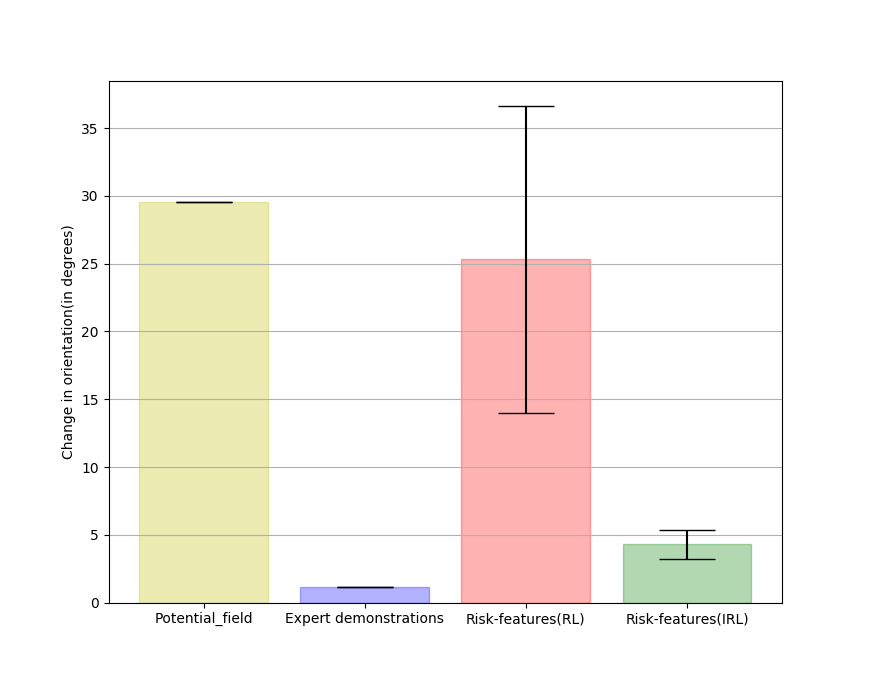
\includegraphics[width=0.7\linewidth]{plots/plot_without_outliers/ucy_inter_method_no_outlier/compute_trajectory_smoothness_ucy_no_outlier_inter_method.png}
    \caption{Average change in the orientation (in degrees) of different agents across multiple trajectories.}
    \label{fig:inter_method-change_in_orientation_avg}
\end{figure}
While PF agents are good navigators, their lack motivation for smooth, controlled movement. A slight change in the configuration of the nearby obstacles can significantly change the potential field around it. This instability reflects in  \autoref{fig:inter_method-change_in_orientation_avg}, where the PF agent, on average, changes its orientation by almost $29.56\degree$ per frame as compared to the $4.29\degree$ of the IRL agent. The RL agent is trained on a simple goal-centric reward function that lacks motivation for optimizing for smoothness. This might be a possible reason for having a high average rotation per frame, and producing irregular movement patterns like the potential field controller. \autoref{tab:inter_method_numerical_results} shows a comparison of the different methods.

%\begin{figure}[!htbp]
%    \begin{subfigure}{\textwidth}
%        \centering
%        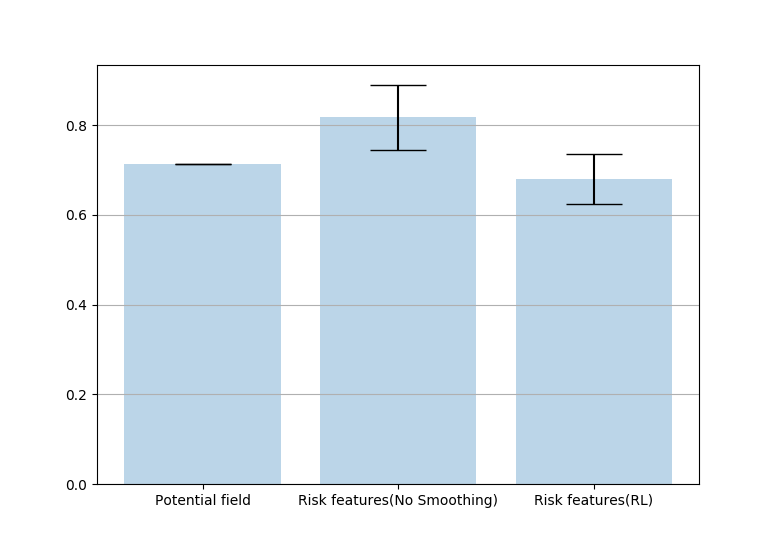
\includegraphics[width=.7\linewidth]{plots/inter_method/distance_displacement_ratio.png}
%        \caption{Histogram plot of distance displacement ratio.}
%        \label{fig:inter_method-distance_disp_ratio}
%    \end{subfigure}
%    \begin{subfigure}{\textwidth}
%        \centering
%        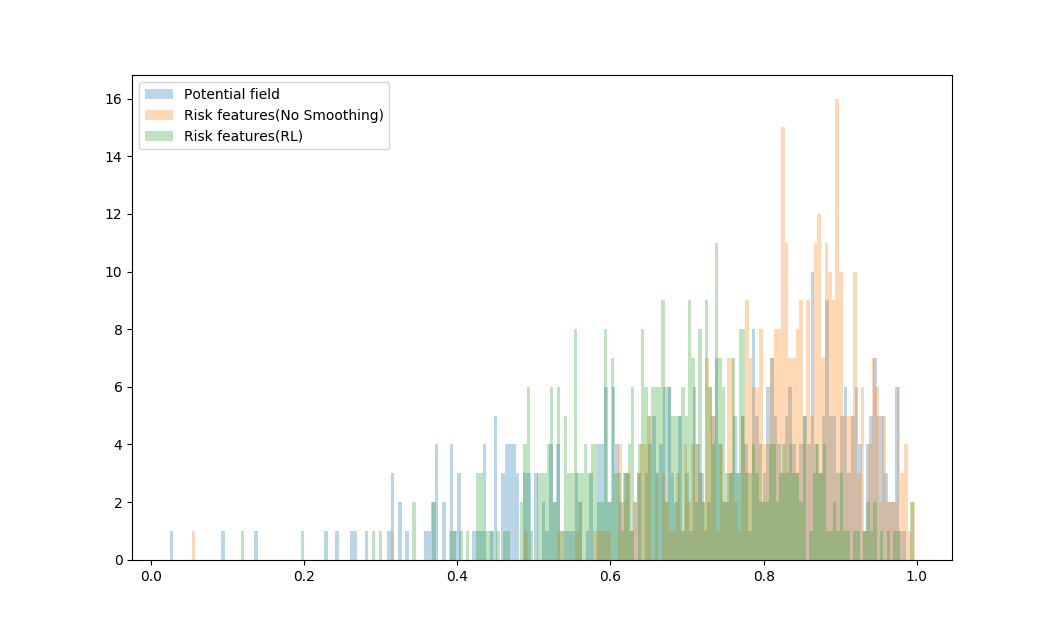
\includegraphics[width=.95\linewidth]{plots/inter_method/histplot_displacement_ratio.png}
%        \caption{Histogram plot of distance displacement ratio.}
%        \label{fig:inter_method-distance_disp_ratio_histplot}
%    \end{subfigure}
%    \caption{Comparing the efficiency of the path taken by the different agents to reach their goals}
%\end{figure}

%Figure \ref{fig:inter_method-distance_disp_ratio} shows that the IRL agent tends to produce more effective trajectories at a distance-displacement ratio of $0.81$ as compared to the $0.71$ and $0.67$ of the PF and RL agent respectively. Figure \ref{fig:inter_method-distance_disp_ratio_histplot} provides a more detailed insight on the distribution of the same over all the trajectories. It shows that for the IRL based agent most of the runs are clustered around the range of $0.8 - 0.9$, and while the PF agent does have a higher density in the range of $0.9 - 1.0$, its distribution is spread over a wider range, with significant number of samples in the sub $0.5$ range. The RL agent on the other hand has a distribution similar to that of the IRL, but with the mean more towards the mid $0.70s$. 


\begin{table}[htbp]
	\begin{center}
		\renewcommand{\arraystretch}{1.3}
		\begin{tabular}{|c|c|c|c|c|}
			\hline
			\textbf{Metric Name} & \textbf{Potential Field} & \textbf{RL} & \textbf{IRL}  &  \textbf{Ground Truth} \\
			\hline
			Goal reached (in $\%$) & $75.11$ & $40.20$ & $65.30$ & $91.16$\\
			Collisions encountered (per run) & $ 0.12$ & $0.20$ & $0.11$ & $0.10$\\
			Change in orientation ( $\degree$ per frame) & $29.56$ & $25.31$ &  $4.29$ & $1.12$ \\
			%Displacement to Distance ratio & $0.71$ & $0.67$ & $0.81$ & $0.84$ \\
			\hline
		\end{tabular}
	\end{center}
	\caption{Score obtained by the different feature representations across different metrics}
	\label{tab:inter_method_numerical_results}
\end{table}
\autoref{fig:inter_method-drift_analysis_all} shows that at any given interval the IRL agent suffers the least amount of deviation when calculated over the set of all the pedestrians. The results from the pedestrian groups of varying difficulty provides more insight. The agents trend to deviate more in easier levels of difficulty as shown in \autoref{fig:inter_method-drift_analysis_easy}, \autoref{fig:inter_method-drift_analysis_med}, \autoref{fig:inter_method-drift_analysis_hard}. A possible explanation to this can be that with the reduction in density of pedestrians nearby, the agent has less incentive to follow the `ground truth' path traced by the original pedestrian as a scant crowd increases the option of available good paths. As the difficulty increases, the room for taking good alternative trajectories decreases and so does the deviation with the IRL agent being the quickest to conform to the expert trajectory not only displaying the least deviation but also producing the biggest reduction in deviation. An exception to the trend is the performance of the potential field controller on the pedestrian set with the highest difficulty. From the formulation of potential field, we know that the force is inversely proportional to the distance between nearby obstacles. In a scene with a large number of pedestrians in the vicinity, the potential field controller, is subjected to a relatively high repulsive force that motivates it to avoid the pedestrians. And while it successfully does so, (low collision rate), it does so by taking irregular trajectories (high rotation rate) which are very different from the ones taken by humans (high amounts of deviation). Another characteristic of all the deviation-plots is that without fail the value of deviation experienced by an agent is more in the longer intervals. This is because an increase in interval denotes a longer distance over which a agent has to plan its trajectory which in turn introduces more autonomy and a greater chance of diverging from the original trajectory traced by the expert.

%
%As the difficulty increases, all the agents show reduced drift, with the IRL agent enjoying significantly lower values as compared to the other. This implies that the rate of resemblance.
%An extreme case on the opposite spectrum would be when only one single trajectory is a collision free path that reaches the goal, in that case, all the successful agents should follow the exact trajectory traced by the pedestrian. For all the in-between cases, successful trajectories can be classified into ones that conform to pedestrians and not. Our method conform more to the pedestrians as compared to the rest.
\begin{figure}[htbp]
	\begin{subfigure}{0.5\textwidth}
		\centering
		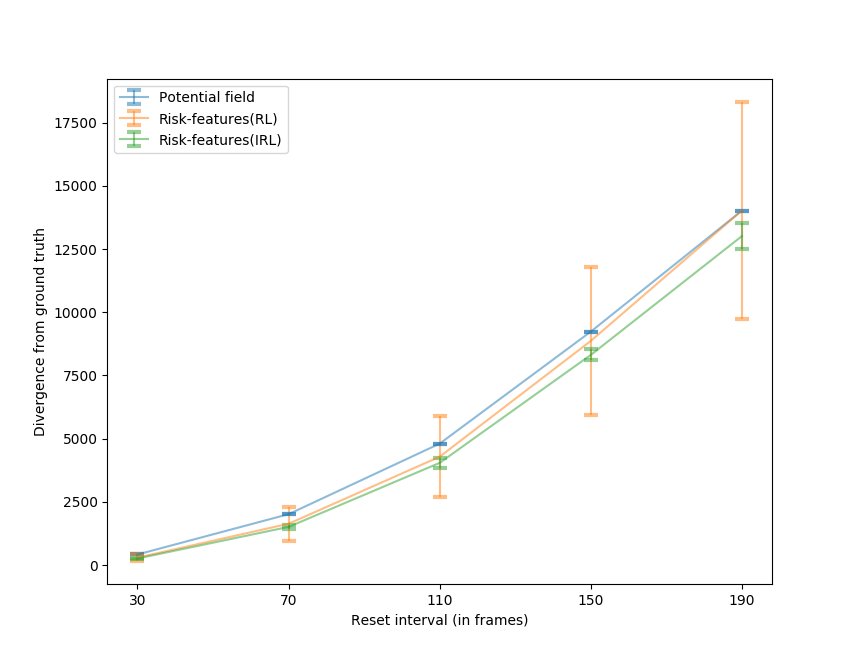
\includegraphics[width=\linewidth]{plots/plot_without_outliers/ucy_inter_method_no_outlier/drift_analysis_easy_no_outliers.png}
		\caption{Deviation from expert experienced by different methods over the easy pedestrians.}
		\label{fig:inter_method-drift_analysis_easy}
	\end{subfigure}
	\begin{subfigure}{0.5\textwidth}
		\centering
		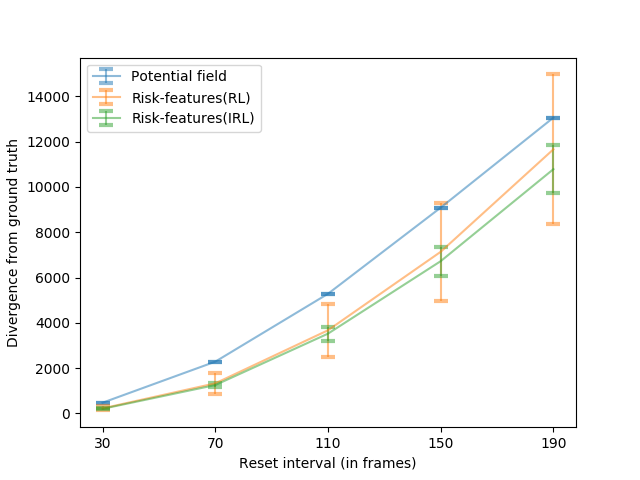
\includegraphics[width=\linewidth]{plots/plot_without_outliers/ucy_inter_method_no_outlier/drift_analysis_med_no_outliers.png}
		\caption{Deviation from expert experienced by different methods over the moderate pedestrians.}
		\label{fig:inter_method-drift_analysis_med}
	\end{subfigure}
	\begin{subfigure}{0.5\textwidth}
		\centering
		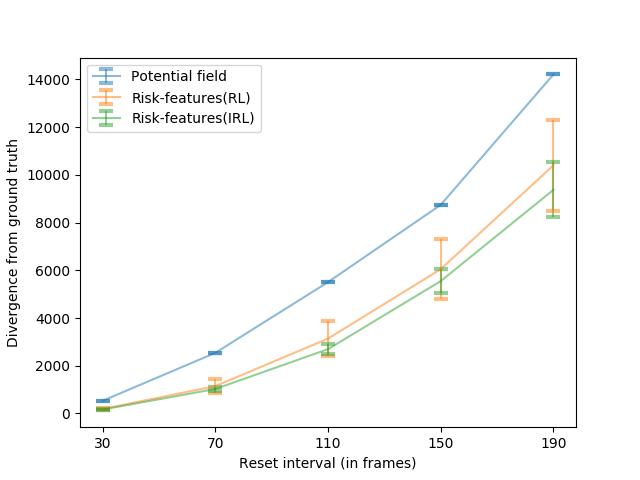
\includegraphics[width=\linewidth]{plots/plot_without_outliers/ucy_inter_method_no_outlier/drift_analysis_hard_no_outliers.png}
		\caption{Deviation from expert experienced by different methods over the hard pedestrians.}
		\label{fig:inter_method-drift_analysis_hard}
	\end{subfigure}
	\begin{subfigure}{0.5\textwidth}
		\centering
		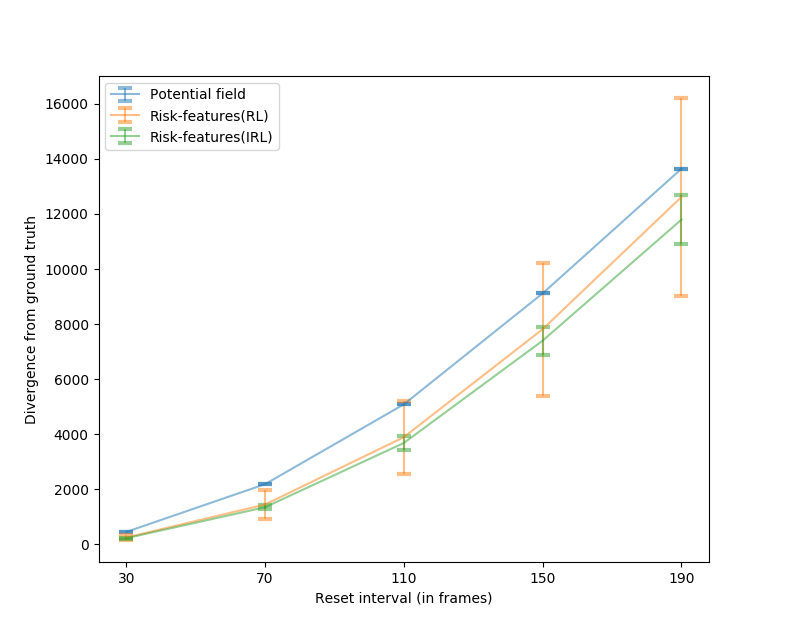
\includegraphics[width=\linewidth]{plots/plot_without_outliers/ucy_inter_method_no_outlier/drift_analysis_all_no_outliers.png}
		\caption{Deviation from expert experienced by different methods over all the pedestrians.}
		\label{fig:inter_method-drift_analysis_all}
	\end{subfigure}
	\caption{Deviation from expert of different agents trained using different methods on the UCY university students dataset.}
\end{figure}

\begin{table}[htbp]
	\begin{center}
		\renewcommand{\arraystretch}{1.3}
		\begin{tabular}{|c|c|c|c|c|c|c|}
			\hline
			 \multicolumn{1}{|c|}{\multirow{2}{*}{\textbf{Agent}}} & \multicolumn{1}{c|}{\multirow{2}{*}{\textbf{Difficulty level}}}  & \multicolumn{5}{c|}{\multirow{1}{*}{\textbf{Interval}}}\\ \cline{3-7}
				
			 && \textbf{30} & \textbf{70} & \textbf{110} & \textbf{150}  &  \textbf{190} \\
			\hline
								& Easy & $417.34$ & $2011.70$ & $4804.05$ & $9235.29$ & $14022.90$ \\ \cline{2-7}
			Potential Field & Moderate & $475.91$ & $2287.18$ & $5283.88$ & $9085.77$ & $13057.17$ \\  \cline{2-7}
								& Hard & $529.96$ & $2538.86$ & $5504.33$ & $8742.69$ & $14210.12$ \\
								\hline
		    	 & Easy & $292.17$ & $1632.78$ & $4286.30$ & $8867.51$ & $14028.13$ \\ \cline{2-7}
		    RL	 & Moderate & $224.62$ & $1330.73$ & $3672.95$ & $7136.29$ & $11659.10$ \\ \cline{2-7}
		    	 & Hard & $186.74$ & $1144.88$ & $3136.16$ & $6047.80$ & $10400.95$ \\
							 	\hline
						& Easy & $259.10$ & $1508.30$ & $4042.63$ & $8314.17$ & $13015.44$ \\ \cline{2-7}
				IRL  & Moderate & $207.27$ & $1255.14$ & $3524.00$ & $6722.75$ & $10782.98$ \\ \cline{2-7}
						& Hard & $164.38$ & $1025.16$ & $2694.89$ & $5546.78$ & $9373.695$ \\
			%Displacement to Distance ratio & $0.71$ & $0.67$ & $0.81$ & $0.84$ \\
			\hline
		\end{tabular}
	\end{center}
	\caption{Magnitude of deviation (in pixels) from expert for different methods in UCY university students dataset.}
	\label{tab:ucy_inter_method_drift_results}
\end{table}

\section{Comparing different feature representations}
\label{sec:comparing-other-featreps}
\subsubsection*{Description of the other feature extractors}
To test for the efficacy of our proposed risk-based feature representation, we test agents trained on our training pipeline with different existing feature representations. For this, we use feature representations proposed in \cite{fahad_learning_2018} and \cite{vasquez_inverse_2014} with some minor modifications and adjustments.\\
%\textbf{Fahad}\\
Due to an underwhelming performance of the originally proposed SAM feature representation from \cite{fahad_learning_2018} in our experimental setup, we substitute the part of the feature representation accommodating the goal information originally proposed by the authors with our global feature representation. We call this modified version the `Goal augmented SAM'.\\
%\textbf{Vasquez}\\
We use the feature sets $\mathcal{F}_1$, $\mathcal{F}_2$ and $\mathcal{F}_3$ from \cite{vasquez_inverse_2014} and as before substitute their goal related features with ours.
To compare against ours, we pick the feature sets $\mathcal{F}_1$, and $\mathcal{F}_3$, the two best performers out of the three representations in our tests.\\
%\textbf{Discuss the results}
\begin{figure}[!htbp]
	\begin{subfigure}{.5\textwidth}
		\centering
		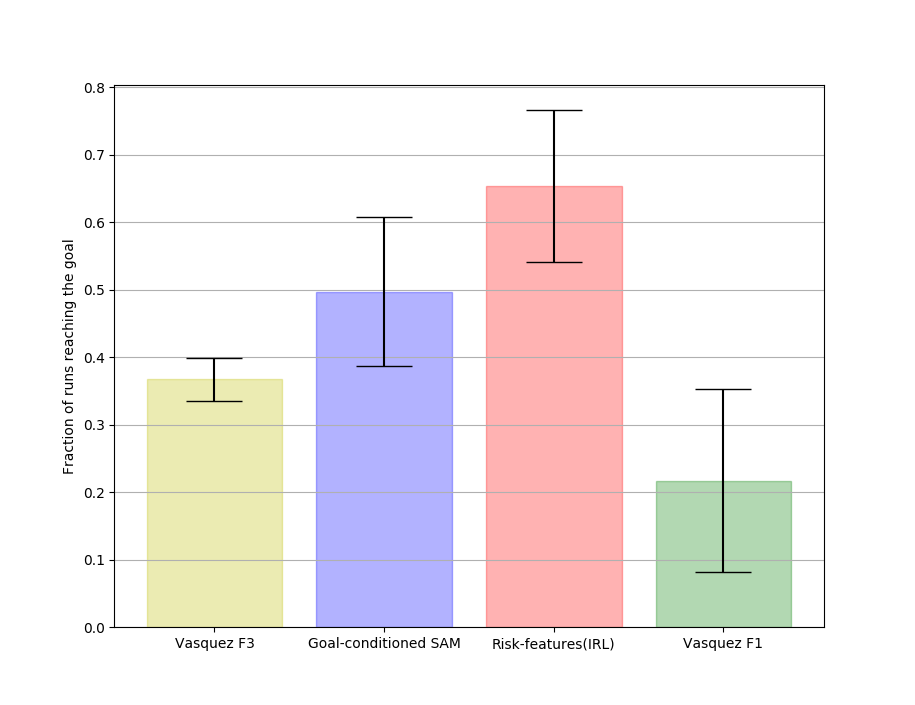
\includegraphics[width=\linewidth, height=6cm]{plots/plot_without_outliers/ucy_inter_irl_no_outliers/goal_reached_ucy_no_outlier_inter_irl.png}
		\caption{Fraction of the runs where the agent succeeds in reaching the goal}
		\label{fig:inter_IRL-goal_reached}
	\end{subfigure}
	\begin{subfigure}{.5\textwidth}
		\centering
		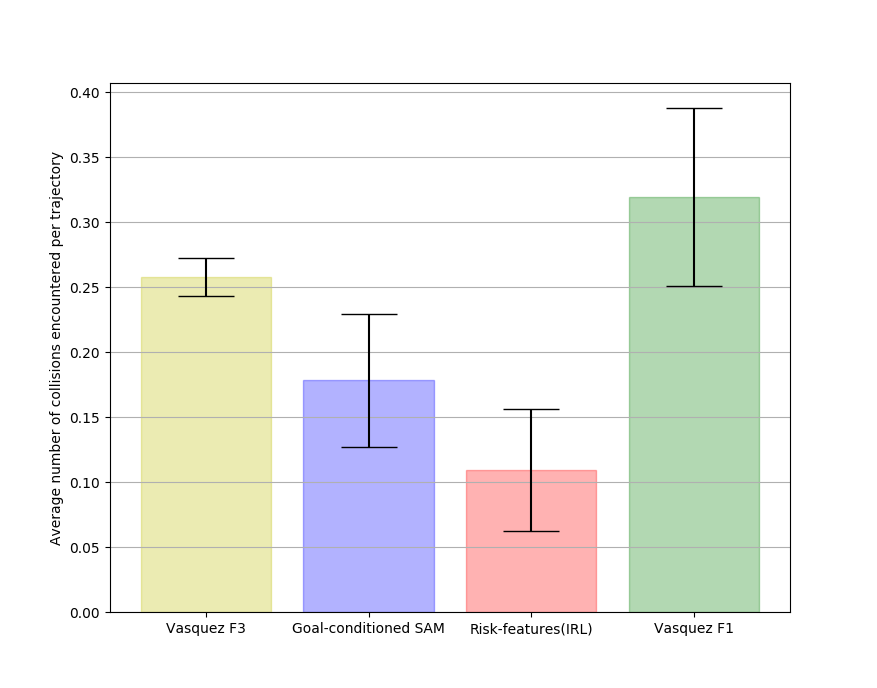
\includegraphics[width=\linewidth, height=6cm]{plots/plot_without_outliers/ucy_inter_irl_no_outliers/count_collisions_ucy_no_outlier_inter_irl.png}
		\caption{Average number of collisions encountered by the agent per trajectory.}
		\label{fig:inter_IRL-collision_counts}
	\end{subfigure}
	\caption{Comparing the fundamental requirements for navigation of different feature representations }
\end{figure}

\begin{figure}[htbp]
	\centering
	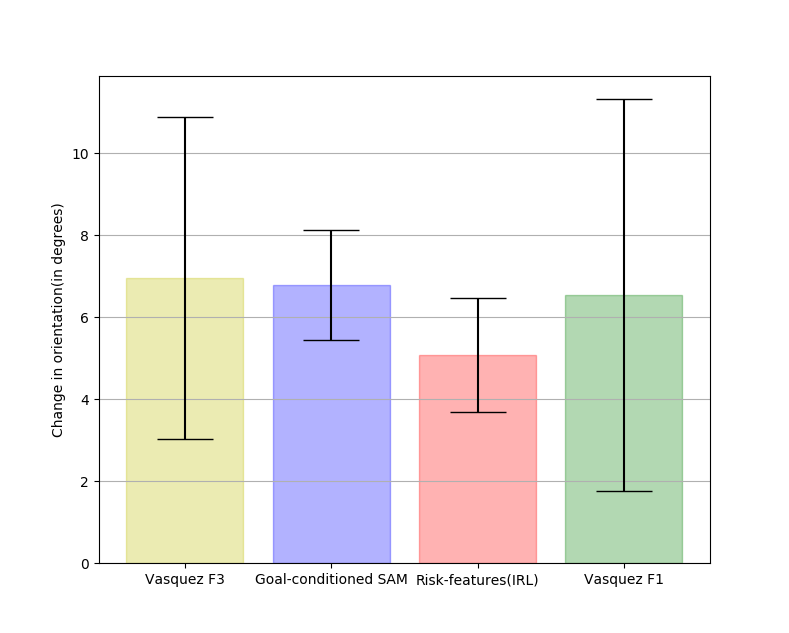
\includegraphics[width=0.7\linewidth]{plots/plot_without_outliers/ucy_inter_irl_no_outliers/compute_trajectory_smoothness_ucy_no_outliers_traj_0.png}
	\caption{Average change in orientation of different agents.}
	\label{fig:inter_IRL-change_in_orientation_avg}
\end{figure}

%\begin{figure}[htbp]
%	\begin{subfigure}{\textwidth}
%		\centering
%		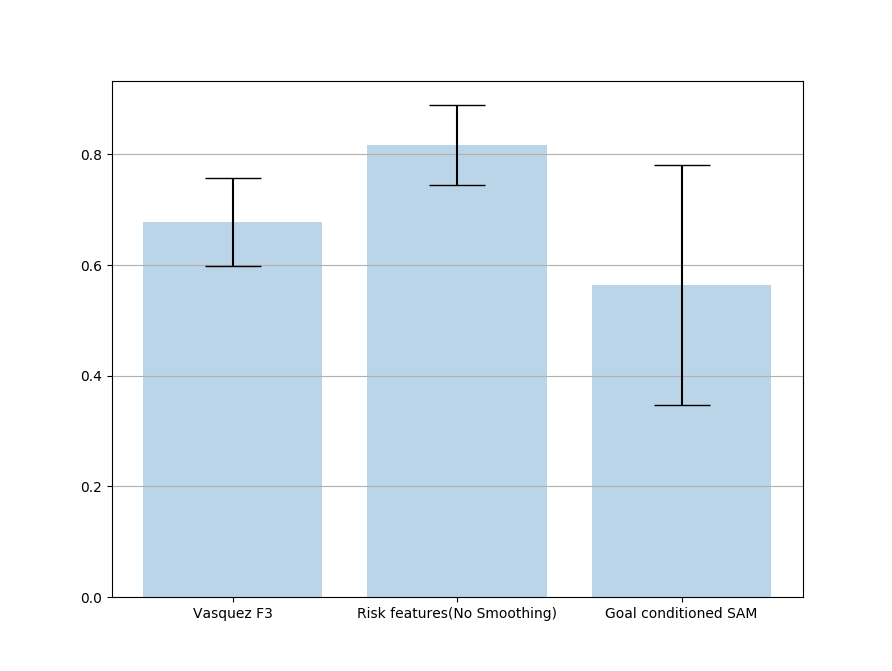
\includegraphics[width=.7\linewidth]{plots/inter_IRL/distance_displacement_ratio_barplots.png}
%		\caption{Histogram plot of distance displacement ratio.}
%		\label{fig:inter_IRL-distance_disp_ratio}
%	\end{subfigure}
%	\begin{subfigure}{\textwidth}
%		\centering
%		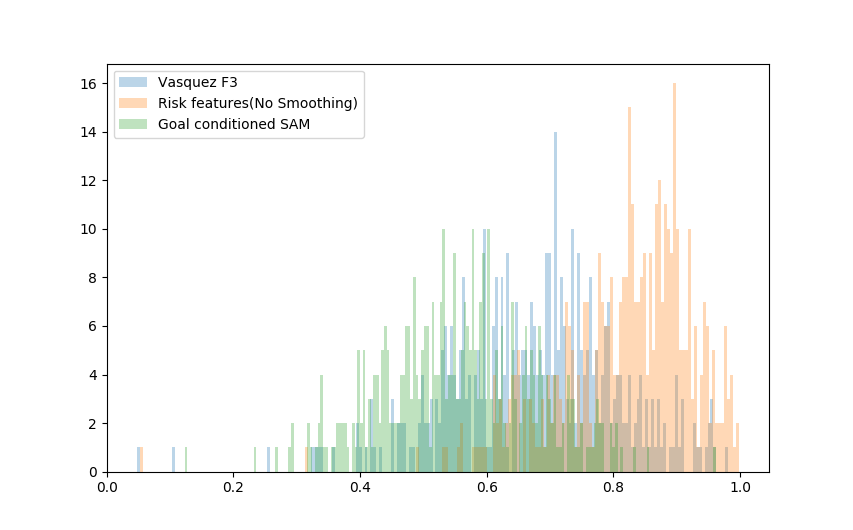
\includegraphics[width=.95\linewidth]{plots/inter_IRL/distance_displacement_ratio_histplot.png}
%		\caption{Histogram plot of distance displacement ratio.}
%		\label{fig:inter_IRL-distance_disp_ratio_histplot}
%	\end{subfigure}
%	\caption{Comparing the efficiency of the path taken by the different agents to reach their goals}
%\end{figure}

We carry out a similar performance analysis as before. \autoref{fig:inter_IRL-goal_reached} and \autoref{fig:inter_IRL-collision_counts} show that in both the fundamental tasks, the risk features outperforms the others with a considerable margin, reaching the goal $65.30\%$ of the times as compared to $21.72\%$, $36.74\%$ and $49.70\%$ of Vasquez $\mathcal{F}1$, Vasquez $\mathcal{F}3$ and Goal-augmented SAM respectively and encountering significantly less collision counts, $0.11$, compared to $0.32$, $0.26$ and $0.17$ from the other  representations. In the subjective evaluation metrics, the results are less pronounced as shown in \autoref{fig:inter_IRL-change_in_orientation_avg}. The risk features undergo a change of $5.08\degree$, $6.54\degree$  by Vasquez $\mathcal{F}1$ which is closely followed by Vasquez $\mathcal{F}3$ and Goal-augmented SAM at $6.59\degree$ and $6.78\degree$ respectively. 
\par
Unlike the comparison of the baseline agents, the performance of the different feature representations at maintaining a smooth trajectory while navigation is comparable. This can be attributed to the use of inverse reinforcement learning to train the agent as the agent learns from demonstration how to behave in crowds.  From the results we infer that all of the feature representations can successfully emulate characteristics of navigation learned from the demonstrations, but the risk features surpass the others at capturing pieces of information from the environment that better convey information like direction of the goal, and the arrangement of obstacles in the neighborhood. This in turn enabled the agent to better grasp the performance of the experts during training and in turn recreate that during testing.%and outperforms the others at making efficient navigation choices producing shorter paths to the goal while avoiding obstacles (Figure. \ref{fig:inter_IRL-distance_disp_ratio_histplot}). 
 \autoref{tab:inter_irl_numerical_comparison} summarizes the scores obtained by the different feature representations.
\begin{table}[htbp]
	\begin{center}
		\renewcommand{\arraystretch}{1.5}
		\begin{tabular}{|p{2.5cm}|c|c|c|c|}
			\hline
			\textbf{Metric Name} & \textbf{Risk Features} & \textbf{Goal-augmented}  & \textbf{Vasquez $\mathcal{F}1$} & \textbf{Vasquez $\mathcal{F}3$}\\
			  &   & \textbf{SAM}  &  &  \\
			\hline
			Goal reached (in $\%$) & $65.30$ & $49.70$ & $21.72$ & $36.74$ \\
			Collisions encountered (per run) & $0.11$ & $0.17$ & $0.32$ & $0.26$\\
			%Change in orientation ( $\degree$ per frame) & $4.29$ & $6.27$ &  $4.08$ & $ 5.02$\\
			Change in orientation ( $\degree$ per frame)  & $5.08$ & $6.78$ &  $6.54$ & $ 6.59$\\ %traj >=0
			\hline
		\end{tabular}
	\end{center}
	\caption{Score obtained by the different feature representations across different metrics}
	\label{tab:inter_irl_numerical_comparison}
\end{table}\\

%drift analysis
\begin{figure}[htbp]
	\begin{subfigure}{0.5\textwidth}
		\centering
		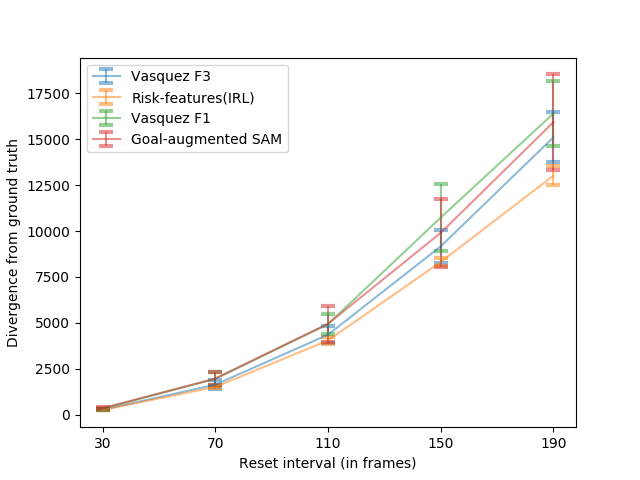
\includegraphics[width=\linewidth]{plots/plot_without_outliers/ucy_inter_irl_no_outliers/ucy_irl_easy.png}
		\caption {Deviation from expert experienced over pedestrians of the easy class.}
		\label{fig:inter_IRL-drift_analysis_easy}
	\end{subfigure}
	\begin{subfigure}{0.5\textwidth}
		\centering
		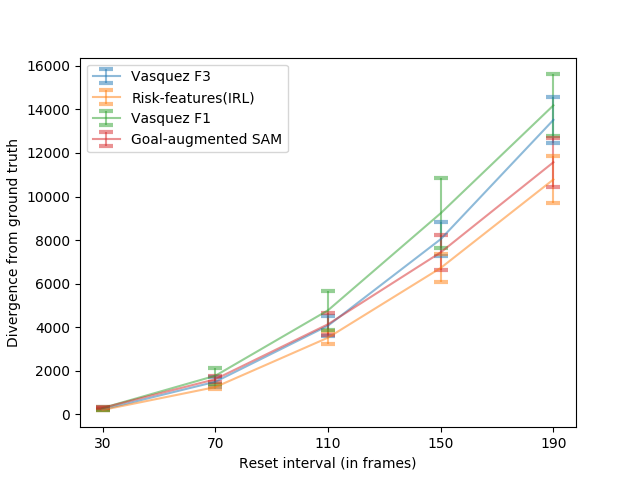
\includegraphics[width=\linewidth]{plots/plot_without_outliers/ucy_inter_irl_no_outliers/ucy_irl_med.png}
		\caption {Deviation from expert experienced over pedestrians of the moderate class.}
		\label{fig:inter_IRL-drift_analysis_med}
	\end{subfigure}
	\begin{subfigure}{0.5\textwidth}
		\centering
		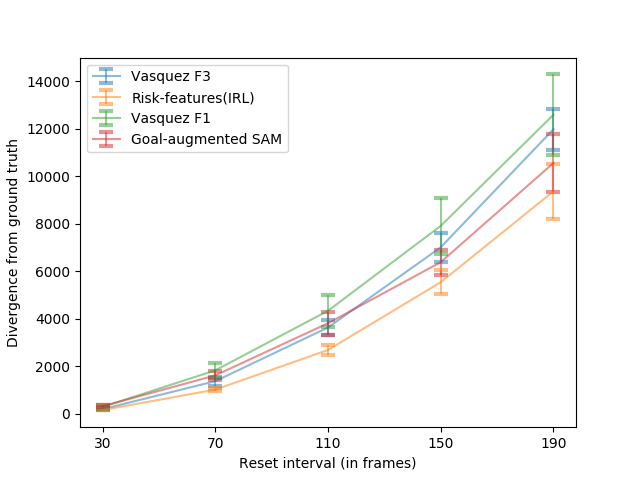
\includegraphics[width=\linewidth]{plots/plot_without_outliers/ucy_inter_irl_no_outliers/ucy_irl_hard.png}
		\caption {Deviation from expert experienced over pedestrians of the difficult class.}
		\label{fig:inter_IRL-drift_analysis_hard}
	\end{subfigure}
	\begin{subfigure}{0.5\textwidth}
		\centering
		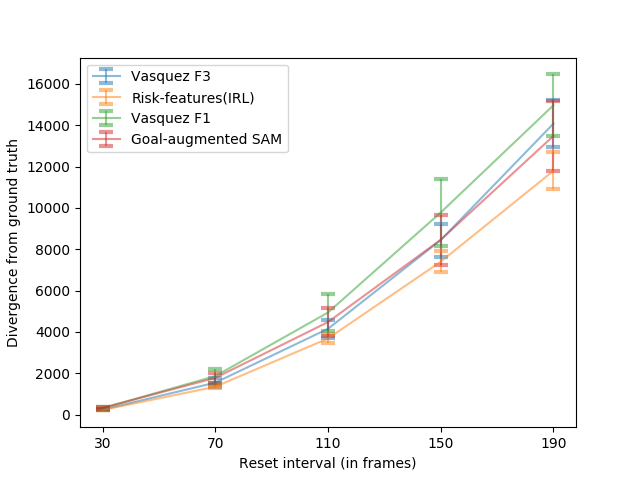
\includegraphics[width=\linewidth]{plots/plot_without_outliers/ucy_inter_irl_no_outliers/ucy_irl_all.png}
		\caption {Deviation from expert experienced over all the pedestrians.}
		\label{fig:inter_IRL-drift_analysis_all}
	\end{subfigure}
	\caption{Deviation from expert experienced by different feature representations on the UCY university students dataset.}
\end{figure}


\begin{table}[htbp]
	\begin{center}
		\renewcommand{\arraystretch}{1.3}
		\begin{tabular}{|c|c|c|c|c|c|c|}
			\hline
			\multicolumn{1}{|c|}{\multirow{2}{*}{\textbf{Agent}}} & \multicolumn{1}{c|}{\multirow{2}{*}{\textbf{Difficulty level}}}  & \multicolumn{5}{c|}{\multirow{1}{*}{\textbf{Interval}}}\\ \cline{3-7}
			
			&& \textbf{30} & \textbf{70} & \textbf{110} & \textbf{150}  &  \textbf{190} \\
			\hline
								& Easy & $259.10$ & $1508.30$ & $4042.63$ & $8314.17$ & $13015.44$ \\ \cline{2-7}
			Risk features & Moderate & $207.27$ & $1255.14$ & $3524.00$ & $6722.75$ & $10782.98$ \\ \cline{2-7}
								& Hard & $164.38$ & $1025.16$ & $2694.89$ & $5546.78$ & $9373.695$ \\
			\hline
											& Easy & $331.79$ & $1974.40$ & $4931.50$ & $10732.14$ & $16397.06$ \\ \cline{2-7}
			Vasquez $\mathcal{F}1$ & Moderate & $293.78$ & $1774.70$ & $4779.41$ & $9233.74$ & $14183.24$ \\ \cline{2-7}
											& Hard & $294.29$ & $1834.67$ & $4343.50$ & $7919.24$ & $12597.04$ \\
			\hline
			 								& Easy & $267.87$ & $1634.24$ & $4355.77$ & $9164.88$ & $15101.88$ \\ \cline{2-7}
			Vasquez $\mathcal{F}3$ & Moderate & $226.58$ & $1499.33$ & $4073.54$ & $8043.44$ & $13516.85$ \\ \cline{2-7}
											& Hard & $200.88$ & $1380.26$ & $3640.10$ & $7016.41$ & $11987.05$ \\
			\hline			
		 							 	& Easy & $351.29$ & $1964.34$ & $4948.78$ & $9901.09$ & $15929.93$ \\ \cline{2-7}
			Goal-augmented SAM & Moderate & $302.65$ & $1615.08$ & $4139.58$ & $7437.50$ & $11573.43$ \\ \cline{2-7}
										& Hard & $324.93$ & $1623.84$ & $3818.54$ & $6390.66$ & $10566.04$ \\
			%Displacement to Distance ratio & $0.71$ & $0.67$ & $0.81$ & $0.84$ \\
			\hline
		\end{tabular}
	\end{center}
	\caption{Magnitude of deviation (in pixels) undergone by different feature representations in UCY university students dataset.}
	\label{tab:ucy_inter_irl_drift_results}
\end{table}


The difference is less pronounced as compared to the agents from different methods. Again we observe that deviation values of every agent tend to increase with the decrease in difficulty of the set of pedestrians being considered. Figures. \ref{fig:inter_IRL-drift_analysis_easy}, \ref{fig:inter_IRL-drift_analysis_med}, \ref{fig:inter_IRL-drift_analysis_hard}), with the risk features consistently outperforming the other representations in all the difficulty levels. This show that the IRL in junction with the risk features produces agents that better reflect human behavior while moving through a social setting while respecting the fundamentals of navigation when compared to other baseline methods and existing feature representations.


\section{Testing for generalization}
\label{sec:generalization}
To test for generalization of the different feature representations, we perform the set of aforementioned tests on the Zara02 dataset: a subset of the UCY dataset. The Zara02 dataset captures a view of a sidewalk in front of a store. It features $203$ pedestrians over a time span of $7$ minutes, making this a relatively sparse scenario in comparison to the UCY university students dataset. As before, we divide the pedestrians into 3 groups based on the average pedestrian density in the vicinity. Out of the $203$ pedestrians, the first $105$ pedestrians with the least density are marked as easy, the next $75$ as moderate and the rest as hard as shown in \autoref{fig:zara02_ped_density_division}. The average density of each division are present in \autoref{tab:zara02_difficulty_level_division}

\begin{figure}[htbp]
	\centering
	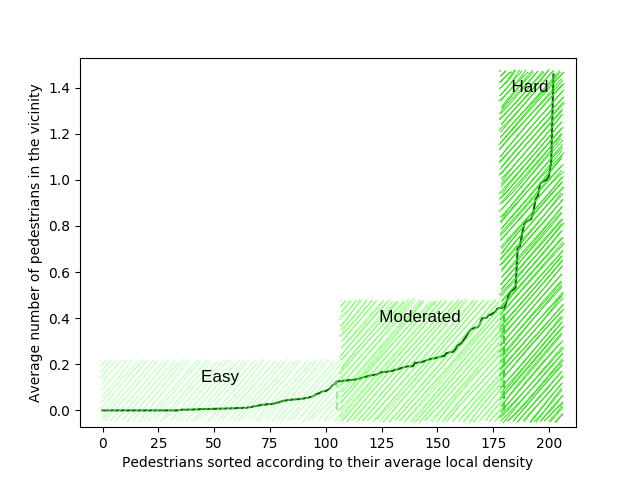
\includegraphics[width=0.8\linewidth]{plots/zara02_ped_density_divisions.png}
	\caption{Classification of the pedestrians of the UCY Zara02 dataset according to the average density of obstacles faced over their trajectories.}
	\label{fig:zara02_ped_density_division}
\end{figure}
\begin{table}[htbp]
	\begin{center}
		\renewcommand{\arraystretch}{1.3}
		\begin{tabular}{|c|c|}
			\hline
			\multirow{2}{*}{\textbf{Difficulty level}} & \textbf{Average pedestrians} \\
			& \textbf{encountered per frame} \\
			\hline
			Easy & $0.017$ \\
			Moderate & $0.20$ \\
			Hard & $0.71$\\
			\hline
		\end{tabular}
	\caption{Average pedestrians encountered at each pedestrian difficulty level}
	\label{tab:zara02_difficulty_level_division}
	\end{center}
\end{table}

\begin{figure}[!htbp]
	\begin{subfigure}[t]{.5\columnwidth}
	\centering
	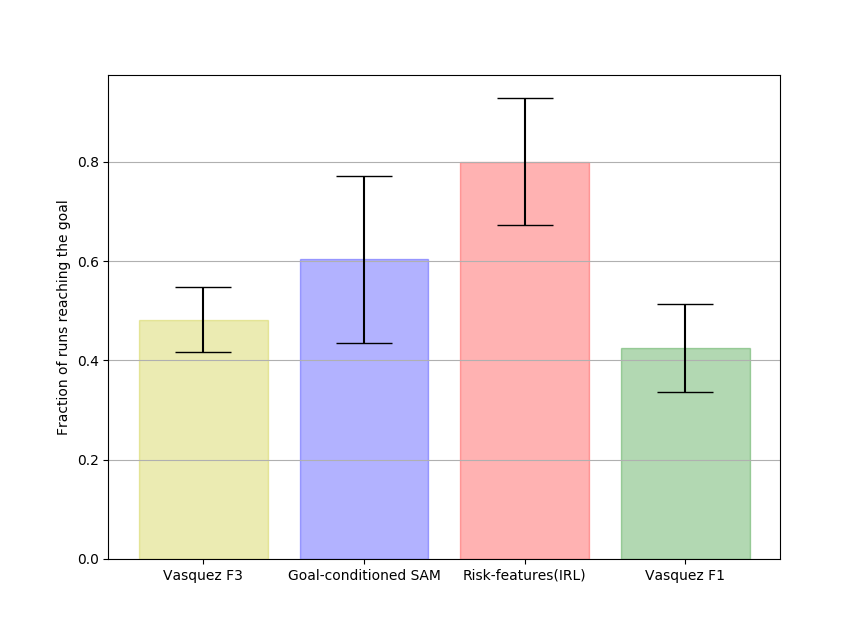
\includegraphics[width=\columnwidth]{plots/plot_without_outliers/zara02_inter_irl_no_outlier/goal_reached_zara02_no_outlier_inter_irl.png}
	\caption{Fraction of runs successfully ending at the goal location for different feature representations.}
	\label{fig:inter_method-goal_reached-zara02}
	\end{subfigure}%
	\begin{subfigure}[t]{.5\columnwidth}
		\centering
		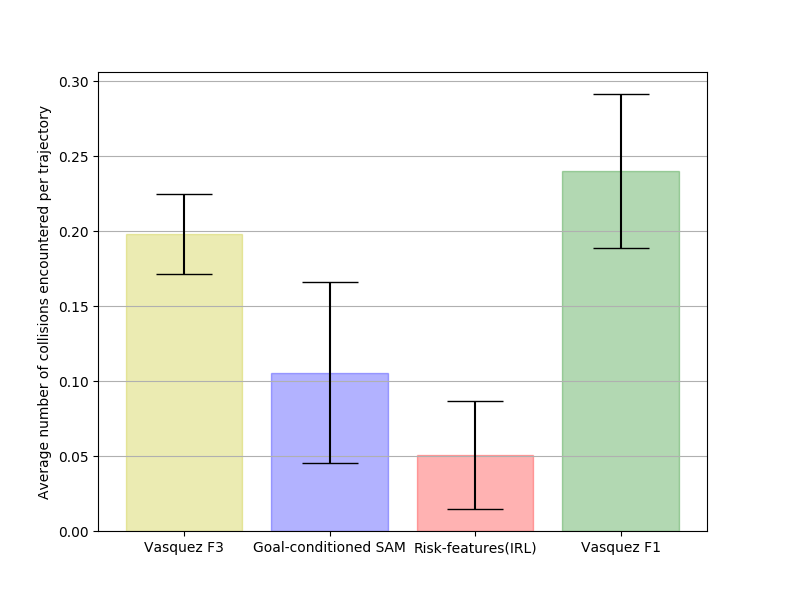
\includegraphics[width=\columnwidth]{plots/plot_without_outliers/zara02_inter_irl_no_outlier/count_collisions_zara02_no_outlier_inter_irl.png}
		\subcaption{Average number of collisions encountered by the different feature representations.}
		\label{fig:inter_method-count_collisions-zara02}
	\end{subfigure}%
	\label{fig:inter_method-classic_navigation_metrics-zara02}
\end{figure}

\begin{figure}[htbp]
	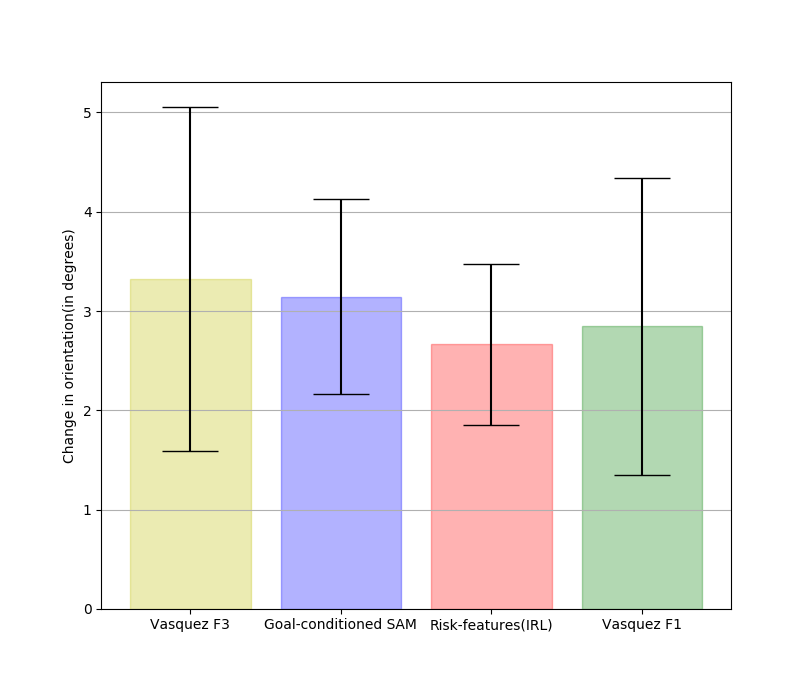
\includegraphics[width=.95\linewidth]{plots/plot_without_outliers/zara02_inter_irl_no_outlier/compute_trajectory_smoothness_zara02_no_outlier_inter_irl_traj_5.png}
	\caption{Average change in orientation per frame for different feature representations.}
	\label{fig:inter_irl-trajectory_smoothness-zara02}
\end{figure}

 The risk features enjoy the highest success rate of reaching the goal at $80.06$, followed by Goal-augmented SAM, Vasquez $\mathcal{F}3$ and Vasquez $\mathcal{F}1$ with a success rate of $60.35$, $42.58$, and $48.25$ respectively.  We also observe a negative correlation between the success rate of reaching the goal and the number of collisions encountered can be observed: with the risk features encountering the least number of average collisions per trajectory at $0.05$ and the Vasquez F1 features on the opposite side of the spectrum averaging $0.24$ collisions per trajectory.  
On the subjective side, the risk features produce the smoothest trajectories, changing its orientation an average of $2.66\degree$ in a dataset that has an average of $0.63\degree$ change observed in the expert demonstrations.\\
Table \autoref{tab:inter_irl_numerical_results_zara02} summarizes the results from the Zara02 dataset.

\begin{table}[htbp]
	\begin{center}
		\renewcommand{\arraystretch}{1.3}
		\begin{tabular}{|p{2.5cm}|c|c|c|c|}
			\hline
			\textbf{Metric Name} & \textbf{Risk Features} & \textbf{Goal-augmented}  & \textbf{Vasquez $\mathcal{F}1$}  & \textbf{Vasquez $\mathcal{F}3$} \\
			&   & \textbf{SAM}  & &  \\
			\hline
			Goal reached (in $\%$) & $80.06$ & $60.35$ & $42.58$ & $48.25$ \\
			Collisions encountered (per run) & $0.05$ & $0.10$ & $ 0.24$ & $0.19$ \\
			%Change in orientation 50 ( $\degree$ per frame) & $2.34$ & $2.65$ &  $2.45$ & $2.41$\\
			Change in orientation ( $\degree$ per frame) & $2.66$ & $3.14$ &  $2.84$ & $3.32$\\ %traj len 5
			\hline
		\end{tabular}
	\end{center}
	\caption{Score obtained by the different feature representations across different metrics}
	\label{tab:inter_irl_numerical_results_zara02}
\end{table}

%drift analysis zara02

\begin{figure}[htbp]
	\begin{subfigure}{0.5\textwidth}
		\centering
		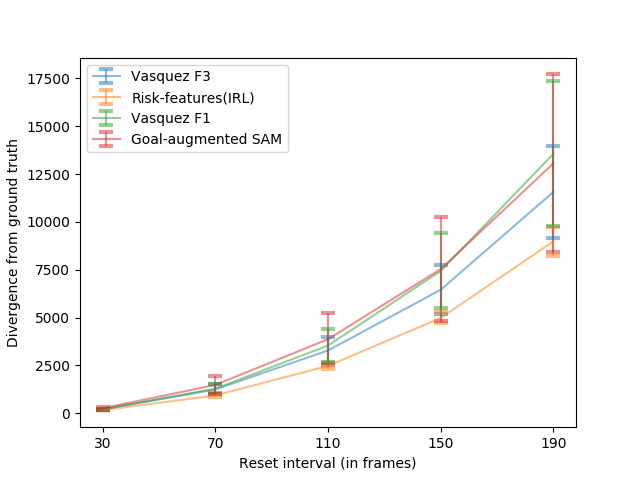
\includegraphics[width=\linewidth]{plots/plot_without_outliers/zara02_inter_irl_no_outlier/Zara02_irl_easy.png}
		\caption {Deviation from expert experienced over the pedestrians of the easy class.}
		\label{fig:inter_IRL-drift_analysis_easy-zara02}
	\end{subfigure}
	\begin{subfigure}{0.5\textwidth}
		\centering
     	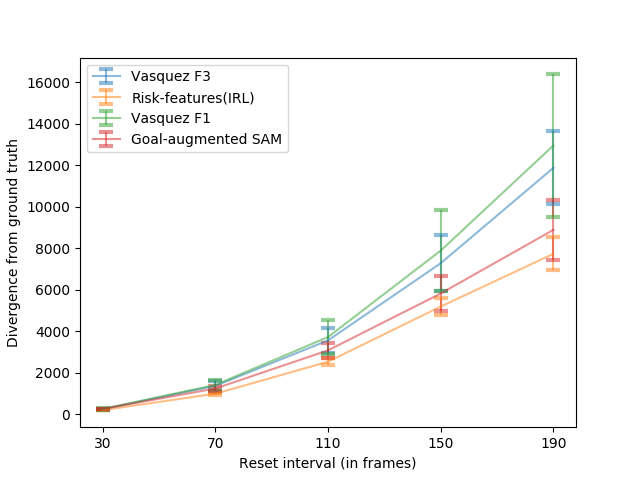
\includegraphics[width=\linewidth]{plots/plot_without_outliers/zara02_inter_irl_no_outlier/Zara02_irl_med.png}
		\caption {Deviation from expert experienced over the pedestrians of the moderate class}
		\label{fig:inter_IRL-drift_analysis_med-zara02}
	\end{subfigure}
	\begin{subfigure}{0.5\textwidth}
		\centering
		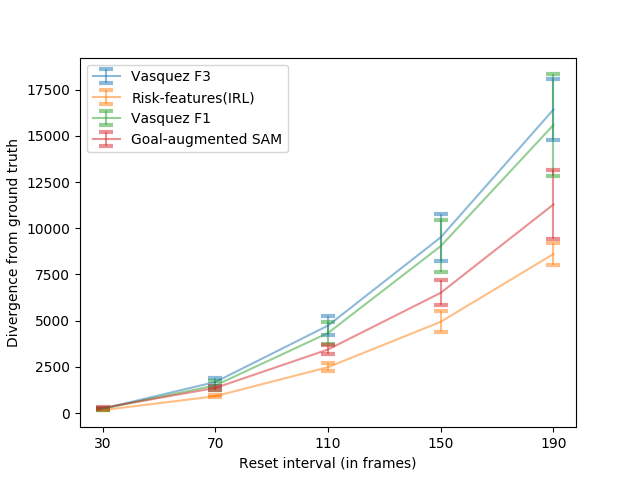
\includegraphics[width=\linewidth]{plots/plot_without_outliers/zara02_inter_irl_no_outlier/Zara02_irl_hard.png}
		\caption {Deviation from expert experienced over the pedestrians of the difficult class}
		\label{fig:inter_IRL-drift_analysis_hard-zara02}
	\end{subfigure}
	\begin{subfigure}{0.5\textwidth}
		\centering
		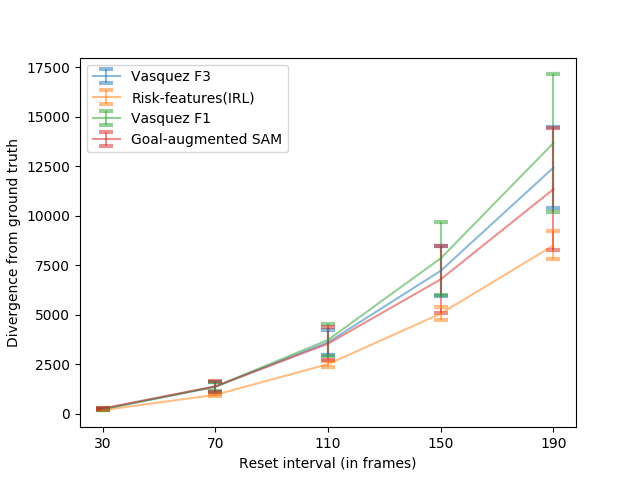
\includegraphics[width=\linewidth]{plots/plot_without_outliers/zara02_inter_irl_no_outlier/Zara02_irl_all.png}
		\caption {Overall deviation from expert experienced over all the pedestrians.}
		\label{fig:inter_IRL-drift_analysis_all-zara02}
	\end{subfigure}
	\caption{Deviation from expert experienced by different feature representations on the UCY Zara02 dataset.}
	\label{fig:drift_analysis-inter_IRL-zara02}
\end{figure}


\begin{table}[htbp]
	\begin{center}
		\renewcommand{\arraystretch}{1.3}
		\begin{tabular}{|c|c|c|c|c|c|c|}
			\hline
			\multicolumn{1}{|c|}{\multirow{2}{*}{\textbf{Agent}}} & \multicolumn{1}{c|}{\multirow{2}{*}{\textbf{Difficulty level}}}  & \multicolumn{5}{c|}{\multirow{1}{*}{\textbf{Interval}}}\\ \cline{3-7}
			
			&& \textbf{30} & \textbf{70} & \textbf{110} & \textbf{150}  &  \textbf{190} \\
			\hline
		    & Easy & $159.27$ & $952.73 $ & $2473.52$ & $4982.58$ & $8985.95 $ \\ \cline{2-7}
			Risk features 	& Moderate & $192.84$ & $985.33 $ & $2528.58$ & $5191.57$ & $7735.49 $ \\ \cline{2-7}
			& Hard & $156.16$ & $909.62 $ & $2482.29$ & $4938.37$ & $8605.43 $ \\
			\hline
			& Easy & $206.30$ & $1282.88$ & $3536.66$ & $7438.34 $ & $13562.75$ \\ \cline{2-7}
			Vasquez $\mathcal{F}1$  & Moderate & $250.43$ & $1407.54$ & $3719.27$ & $7889.18$ & $12960.74$ \\ \cline{2-7}
			& Hard & $231.17$ & $1493.02$ & $4330.47$ & $9032.76$ & $15586.48$ \\
			\hline
			& Easy & $198.17$ & $1241.53$ & $3279.74$ & $6455.54$ & $11569.65$ \\ \cline{2-7}
	    	Vasquez $\mathcal{F}3$ 	& Moderate & $234.40$ & $1365.36$ & $3556.70$ & $7280.97$ & $11881.93$ \\ \cline{2-7}
			& Hard & $232.59$ & $1677.60$ & $4731.14$ & $9509.05$ & $16422.56$ \\
			\hline			
			& Easy & $258.47$ & $1477.45$ & $3869.17$ & $7533.29$ & $13064.31$ \\ \cline{2-7}
			Goal-augmented SAM  & Moderate & $251.04$ & $1235.15$ & $3076.86$ & $5821.04$ & $8890.96 $ \\ \cline{2-7}
			& Hard & $275.43$ & $1356.22$ & $3437.67$ & $6506.27$ & $11286.85$ \\
			%Displacement to Distance ratio & $0.71$ & $0.67$ & $0.81$ & $0.84$ \\
			\hline
		\end{tabular}
	\end{center}
	\caption{Magnitude of deviation (in pixels) undergone by different feature representations in UCY Zara02 dataset.}
	\label{tab:zara02_inter_irl_drift_results}
\end{table}

\autoref{fig:drift_analysis-inter_IRL-zara02} show that the risk features outperform its counterparts, adhering more to the trajectories traced by the expert demonstrations compared to any other existing feature representations. The experiments conducted show that along with a better representation, more meaningful representation of the environment, the risk features are also better at generalizing for previously unseen states from different data distributions.

We conduct $3$ sets of experiments first, each aimed for a specific goal. The baseline section compares the performance of different methods providing insight on how inverse reinforcement learning methods compare against some other forms of approach used in the literature. Feature representation plays a major role in the performance of an IRL agent. To test the efficacy of our proposed representation, we fix the training process and alter the feature representation effectively performing an ablation study. Finally, we conduct a generalizability test to study the performance of the different feature representations in a novel setting. We employ various metrics, both subjective and objective to evaluate the performance of the agents. Evaluation of the agents, especially in metrics like trajectory smoothness and deviation from expert comes with its own set of challenges. Calculation of trajectory smoothness is straight forward, but there are various cases that needs to be considered in order to get a true reflection of the performance. For example, let us consider two agents: one never changes its direction and keeps moving forward until termination via reaching the goal or otherwise, and the other actively sidesteps to avoid obstacles and steers towards the goal. Focusing only on the smoothness of their trajectories and placing the first agent ahead of the second, while objectively true, does not convey the true performance, because in this case, the first agent receives a lower, more desired score, by the virtue of being an inadequate navigator who fails to respond to external entities. Similarly, calculation of the deviation is based on the assumption that there is only one optimal trajectory for a particular situation, which in most case is too restrictive of an assumption.
%\subsection*{Testing on custom scenarios}
%\textbf{Follow the group}
%follow\_the\_group\_1.txt(subject 5)
%follow\_the\_group\_3.txt(subject 2)
%\textbf{Passing}
%
%\textbf{t-junctions}
%
%\textbf{avoiding group}
%
%\subsection*{Understanding the reward function}
%Something that is mostly forgotten if you look at most of the navigation-related work. They never discuss the results.


\chapter{Final Conclusion \& Future Work}
\label{part:conclusion}
\label{ch:conclusion}
\section{Conclusion}
In this work, we improve on existing MEDIRL based navigation pipelines by introducing a new `risk-based' feature representation and a sampling technique to operate in a model-free environment. \\
Unlike the majority of the existing literature that focuses on navigation in fairly restricted environments such as narrow hallways or synthetically created scenarios, we opt for a more general and therefore challenging setting: a busy university campus which includes pedestrians with a wide range of people in the vicinity. With no hard restriction on the pathways, the only constraint posed is in the form of social interaction. Additionally, we use a small dataset: $430$ trajectories extracted from a three and a half minute video showcasing the capability of the pipeline to learn using a relatively small set of expert demonstrations.\\
Next, we present a detailed analysis comparing both qualitative and quantitative performance of agents trained using different methods: artificial potential fields, reinforcement learning(actor-critic), inverse reinforcement learning(MEDIRL); and different feature representations from the existing literature in tandem with IRL showcasing the strengths and weaknesses of different approaches.\\
Lastly, in the process, we present a lightweight OpenAI-based environment using Pygame specifically designed for navigation tasks in a social environment which includes features like using annotation files from real-world videos to populate the environment, creating custom navigation scenarios and user control of the agent to collect expert demonstrations among others. \\
There are a few caveats from MEDIRL that trickle-down in the proposed navigation pipeline. Although it leads to improved performance, we are still relying on handcrafted feature representations to make sense of our agent's surroundings. \\

\section{Future Work}
There is possible room for improvement that can be interesting to explore. The performance of learning models heavily depend on the data being used. We use a relatively small dataset to train our models and obtain a competent controller with reasonable performance. Switching to a more comprehensive data, preferably one obtained from a large, indoor space with minimal restriction on the movements of the crowd from any other entity barring pedestrians. 
\\
Maximum entropy inverse reinforcement learning has been the choice of algorithm in the field of social navigation. A drawback of the method is the repeated optimization of a reinforcement learning agent at every update of the reward network. This vastly increases the training time of the algorithm. Exploring different methods that bypass this, like Guided cost learning (GCL) \cite{finn2016gcl} and Generative adversarial imitation learning (GAIL) \cite{ho2016gail} would be one of our priorities in the future.  
\\
Metrics are vital in the context of social navigation or research in general. A set of effective, and standard metrics can help us successfully evaluate the performance of an agent objectively, and carry out unbiased comparison with existing work in the same domain. The formulating and maintenance a set of universally accepted set of metrics that can reasonably gauge the 'social' performance of a navigating agent can be a possible area of focus.
\\
For a project on socially acceptable navigation, the end result is a functioning robot that successfully moves among people in the real world abiding by explicit and tacit social and cultural norms of the society. Another goal to pursue would be moving from simulation to the real world which comes with its own set of challenges including but not limited to error in sensor reading, failure in hardware, encounter with unknown circumstances.
\\
\section{Final remarks}
With the increase in deployment of robots alongside humans, social navigation is a problem that is more relevant that ever. This thesis builds upon work in the existing literature, improving certain components leading to a better navigation agent. We hope that the work presented here are steps in the direction of solving the problem and aid in the realization of having social autonomous robots as a part of the future society.

%The controller can also be used for prediction.
%End to end model removing the need for hand-engineered feature representations.
%use of a hierarchical control architecture to control different aspects of navigation.
%Can be deployed in real-world robots

\begin{onehalfspacing}


%\chapter*{{\huge\rm\bfseries{List of Publications}}}
%\addcontentsline{toc}{chapter}{List of Publications}


\chapter*{\rm\bfseries List of Publications}
\chaptermark{{\rm\bfseries List of Publications}}
\addcontentsline{toc}{chapter}{List of Publications}










\vspace{0.0cm}
\noindent
\textit{Published:}



%\begin{tabularx}{\textwidth}{ l lll }

\begin{itemize}

\item My Papers



\end{itemize}

\end{onehalfspacing}


\newpage

%%%%%%%%%%%%%%%%%%%
%
% BIBLIOGRAPHY
%
%%%%%%%%%%%%%%%%%%%


%\chapter*{\rm\bfseries Bibliography}
\chaptermark{{\rm\bfseries Bibliography}}
\addcontentsline{toc}{chapter}{Bibliography}

\bibliographystyle{alpha}
\bibliography{Thesis}

%\addcontentsline{toc}{chapter}{\numberline{}\rm\bfseries{Bibliography}}

\begin{onehalfspacing}

\chapter*{{\huge\rm\bfseries{Acronyms}}}

\addcontentsline{toc}{chapter}{Acronyms}
\scriptsize
\begin{table}[!h]
\vspace{-2.0cm}
\hspace{1.0cm}
\begin{tabular}{l l r}

\textsc{MDP}  &  Markov Decision Process\\ [2ex]
\textsc{RL}  &  Reinforcement Learning \\ [2ex]
\textsc{IRL}  &  Inverse Reinforcement Learning \\ [2ex]
\textsc{MEDIRL}  &  Maximum Entropy Deep Inverse Reinforcement Learning\\ [2ex]
\textsc{MAP-BIRL}  &  Maximum-a-posteriori Bayesian Inverse Reinforcement Learning\\ [2ex]
\textsc{3D}  &  Three Dimensional\\ [2ex]
\textsc{A2C}  &  Advantage Actor Critic \\ [2ex]
\textsc{GCL}  &  Guided Cost Learning Address Translation \\ [2ex]
\textsc{GAIL}  &  Generative Adversarial Imitation Learning \\ [2ex]
\textsc{SAM}  &  Social Affinity Map \\ [2ex]
\textsc{PF}  &  Network Address Translation \\ [2ex]
\textsc{UCY}  &  University of Cyprus \\ [2ex]
\textsc{RRT}  &  Rapidly exploring Random Tree\\ [2ex]
\textsc{LSTM}  &  Long Short-Term Memory\\ [2ex]
\textsc{ROS}  &  Robot Operating System\\ [2ex]
\textsc{RGB-d}  &  Red Green Blue depth\\ [2ex]

\textsc{SVF}  &  State Visitation Frequency\\ [2ex]
\textsc{ELU}  &  Exponential Linear Units\\ [2ex]
\textsc{MSE}  &  Mean Square Error\\ [2ex]
\end{tabular}
\end{table}











\end{onehalfspacing}

\normalsize
\printindex

%%%%%%%%%%%%%%%%%%%
%
% APPENDICES
%
%%%%%%%%%%%%%%%%%%%

% \appendix


% \input{content/ConsADExamples.tex}

\end{document}
